% -*- coding: utf-8 -*-
\chapter{Компиляция~в~Си}\label{chapter:cc}

\indexR{язык!целевой}
\initial{0.25ex}{0.0ex}{И}{\kern0.95ex ещё одна глава} о~компиляции. Но в~этот
раз мы разберём несколько новых подходов, в~частности, плоские окружения, а ещё
у~нас сменился целевой язык: теперь им будет~Си. Подобное сочетание языков
поднимает несколько своеобразных вопросов, стоящих рассмотрения. С~одной
стороны, брак с~представителем более высокого сословия сулит определённые
выгоды: например, бесплатные низкоуровневые оптимизации и доступ к~огромному
количеству библиотек на все случаи жизни. Но роз без шипов не~бывает, так что
взамен мы отдаём хвостовую рекурсию и вдобавок получаем кучу проблем со~сборкой
мусора.

\bigskip

\indexR{компиляция!в~язык высокого уровня}
Компиляция в~язык высокого уровня, вроде~Си, интересна во~многих отношениях. Так
как целевой язык несомненно богаче ассемблера, то всё~же можно надеяться на
несколько более близкий к~оригиналу результат, нежели бесформенный ералаш
байт-кодов. Далее, компиляторы~Си существуют практически для любой платформы,
что благотворно сказывается на переносимости. Более того, эти компиляторы
не~вчера родились и имеют в~своём распоряжении существенный арсенал оптимизаций,
а также неплохо справляются с~рутинными низкоуровневыми задачами вроде
распределения регистров, расположения данных в~памяти, выбора режимов адресации
"--- обо~всём этом можно забыть, сфокусировавшись исключительно на
высокоуровневом аспекте компиляции.

С~другой стороны, выбор языка высокого уровня в~качестве целевого накладывает
определённые философские и практические ограничения. Подобные языки обычно
разрабатываются под определённый стиль программирования и, чаще всего, без
особого внимания к~вопросу кодогенерации. В~результате обнаруживаются
разнообразные <<стеклянные стены>> вроде не~более 32~аргументов у~функций, или
16~максимальных уровней вложенности блоков, и так далее. Нормальные пользователи
их даже не~замечают, а вот глупые программы-генераторы то и дело натыкаются.
Бывает, что какой"~то жалкий макрос раздувает программу в~5, 10, а то и в~20~раз
при переводе на Си, а потом этого монстра ещё пытаются скормить компилятору.

Более того, если модель исполнения целевого языка имеет мало общего с~моделью
языка исходного, это плохо сказывается как на сложности самого процесса
преобразования, так и на эффективности использования возможностей целевого
языка. Си разрабатывался как язык системного программирования (изначально для
написания \UNIX), поэтому в~нём намеренно применяется явное управление памятью.
Вследствие этого могут возникать невероятно каверзные ошибки, если программист
не~будет предельно осторожен с~указателями, "--- иначе это лишь вопрос времени,
когда программа выйдет из-под контроля и начнёт творить непоправимое. В~Лиспе
подобная ситуация невозможна в~принципе, это безопасный язык в~плане управления
памятью.

Вдобавок ко~всему, Си не~особо подходит для функционального стиля
программирования, где вызовы функций и рекурсия случаются на каждом шагу.
Компиляторы тщательнее оптимизируют императивные аспекты языка, поэтому
программисты стараются избегать менее эффективных в~данном случае функциональных
алгоритмов, что даёт разработчикам компиляторов моральное право уделять меньше
внимания их оптимизации, так как они всё равно редко используются. Такой вот
замкнутый круг.

Как~бы то ни~было, нельзя сказать, что~Си непопулярен в~качестве целевого языка
компиляции Лиспа. Достаточно упомянуть Kyoto {\CommonLisp} \cite{yh85} (а~также
улучшенный Уильямом~Скэлтером AKCL), WCL \cite{hen92b}, CLICC \cite{hof93},
ECoLisp \cite{att95}, Scheme$\to$C \cite{bar89}, Sqil \cite{sen91}, ILOG~Talk
\cite{ilo94}, Bigloo~\cite{ser94}.

Наш компилятор им не~соперник. Это лишь набросок, однако имеющий достаточное
количество интересных деталей. Конечно, можно было~бы пойти простым путём
(кто"~то поправит: тривиальным) "--- взять компилятор в~байт-код из седьмой
главы \seePage[chapter:compilation] и переработать его, чтобы он выводил код на
Си, а не~байты. Ведь для каждой машинной инструкции определена её операционная
семантика, так что не~составит труда перевести их все на~Си. Однако нас ожидает
совершенно иной путь, пролегающий сквозь страну плоских окружений.
\seePage[fast/fast/variations/ssect:flat] Рассматриваемый компилятор будет
многопроходным. Объектное представление обрабатываемых программ значительно
облегчит их анализ и трансформацию. По сути, именно систематический
объектно"=ориентированный подход делает излагаемый в~данной главе материал столь
элегантным и расширяемым.


\section{Объектификация}\label{cc/sect:objectification}

\indexR{объектификация}
В~разделе~\ref{macros/macrosystem/ssect:object}
\seePage[macros/macrosystem/ssect:object] рассматривался алгоритм преобразования
программ в~объектную форму. Он раскрывает все макросы и в~конечном итоге
возвращает готовый объект класса \ic{Program}. Чтобы разбавить это весьма
лаконичное описание, вашему вниманию предлагается
рисунок~\ref{cc/objectification/pic:result} с~результатом объектификации
следующей далее программы. В~ней, если присмотреться, можно найти каждый
изученный нами существенный аспект Scheme. Страницы не~безграничны, так что
имена классов записаны сокращённо, а часть дерева и вовсе не~показана. На
протяжении этой главы мы не~раз будем возвращаться к~данному примеру.

\begin{code:lisp}
(begin
  (set! index 1)
  ((lambda (cnter . tmp)
     (set! tmp (cnter (lambda (i) (lambda x (cons i x)))))
     (if cnter (cnter tmp) index) )
   (lambda (f)
     (set! index (+ 1 index))
     (f index) )
   'foo) )        |$\is$| (2 3)
\end{code:lisp}

\begin{figure}\centering
% -*- coding: utf-8 -*-
% Объектифицированный код
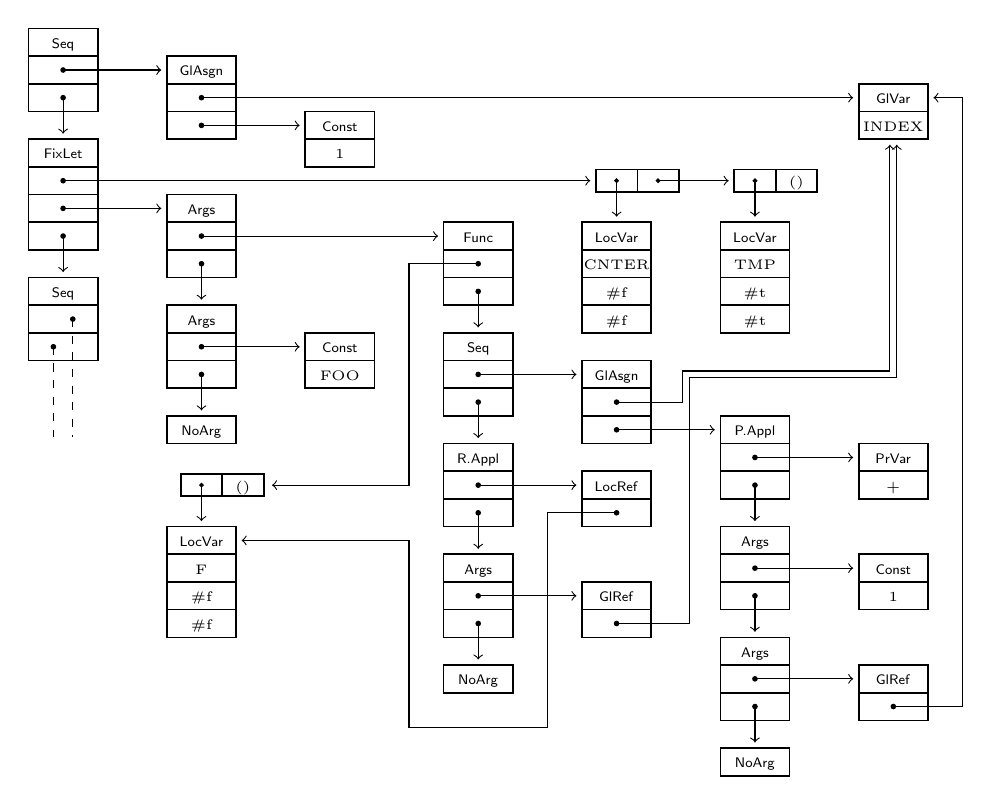
\begin{tikzpicture}
  \tikzstyle{every node}=[font=\tiny]

\def\NodeContent#1{\node [anchor = mid] at(1.25em, -0.5em) {#1};}
\def\NodeTitle#1{\NodeContent{\textsf{#1}}}
\def\NodePtr{\filldraw (1.25em, -0.5em) circle(0.8pt);}
\def\Box{\draw [semithick] (0, 0) rectangle (2.5em, -1.0em);}

\def\InList{%
  \begin{scope}[xshift = +0.5em, yshift = +1.5em]
    \draw [semithick] (0.0em, +0.4em) rectangle (3.0em, -0.4em)
                      (1.5em, +0.4em) -- (1.5em, -0.4em);
    \filldraw (0.75em, 0.0em) circle(0.65pt)
              (2.25em, 0.0em) circle(0.65pt);
  \end{scope}
}

\def\InListLast{%
  \begin{scope}[xshift = +0.5em, yshift = +1.5em]
    \draw [semithick] (0.0em, +0.4em) rectangle (3.0em, -0.4em)
                      (1.5em, +0.4em) -- (1.5em, -0.4em);
    \filldraw (0.75em, 0.0em) circle(0.65pt);
    \node [anchor = mid] at(2.25em, 0.0em) {\ic{()}};
  \end{scope}
}

\def\PullListLink{\draw [->] (-2.25em, 1.5em) -- (0.30em, 1.5em);}

\def\InBotList{%
  \begin{scope}[xshift = +0.5em, yshift = -1.5em]
    \draw [semithick] (0.0em, +0.4em) rectangle (3.0em, -0.4em)
                      (1.5em, +0.4em) -- (1.5em, -0.4em);
    \filldraw (0.75em, 0.0em) circle(0.65pt)
              (2.25em, 0.0em) circle(0.65pt);
  \end{scope}
}

\def\InBotListLast{%
  \begin{scope}[xshift = +0.5em, yshift = -1.5em]
    \draw [semithick] (0.0em, +0.4em) rectangle (3.0em, -0.4em)
                      (1.5em, +0.4em) -- (1.5em, -0.4em);
    \filldraw (0.75em, 0.0em) circle(0.65pt);
    \node [anchor = mid] at(2.25em, 0.0em) {\ic{()}};
  \end{scope}
}

\def\PullBotListLink{\draw [->] (-2.25em, -1.5em) -- (0.30em, -1.5em);}

\def\PullLinkUp{\draw    [->] ( 1.25em,  1.50em) -- ( 1.25em,  0.20em);}
\def\PullLinkLeft{\draw  [->] (-3.75em, -0.50em) -- (-0.20em, -0.50em);}
\def\PullLinkDown{\draw  [->] ( 1.25em, -1.50em) -- ( 1.25em, -0.20em);}
\def\PullLinkRight{\draw [->] ( 6.25em, -0.50em) -- ( 2.70em, -0.50em);}

\def\NoArgNode{%
  \begin{scope}[yshift = -0.0em]
    \Box
    \NodeTitle{NoArg}
  \end{scope}
}

\def\NoFreeNode{%
  \begin{scope}[yshift = -0.0em]
    \Box
    \NodeTitle{NoFree}
  \end{scope}
}

\def\PtrNodeU#1{%
  \begin{scope}[yshift = -0.0em]
    \Box
    \NodeTitle{#1}
  \end{scope}
  \begin{scope}[yshift = -1.0em]
    \Box
    \NodePtr
  \end{scope}
}

\def\ContentNode#1#2{
  \begin{scope}[yshift = -0.0em]
    \Box
    \NodeTitle{#1}
  \end{scope}
  \begin{scope}[yshift = -1.0em]
    \Box
    \NodeContent{#2}
  \end{scope}
}

\def\PtrNodeD#1{%
  \begin{scope}[yshift = -0.0em]
    \Box
    \NodeTitle{#1}
  \end{scope}
  \begin{scope}[yshift = -1.0em]
    \Box
    \NodePtr
  \end{scope}
  \begin{scope}[yshift = -2.0em]
    \Box
    \NodePtr
  \end{scope}
}

\def\ContentNodeD#1#2#3{
  \begin{scope}[yshift = -0.0em]
    \Box
    \NodeTitle{#1}
  \end{scope}
  \begin{scope}[yshift = -1.0em]
    \Box
    \NodeContent{#2}
  \end{scope}
  \begin{scope}[yshift = -2.0em]
    \Box
    \NodeContent{#3}
  \end{scope}
}

\def\PtrNodeDS#1{%
  \begin{scope}[yshift = -0.0em]
    \Box
    \NodeTitle{#1}
  \end{scope}
  \begin{scope}[yshift = -1.0em]
    \Box
    \begin{scope}[xshift = +0.35em]
      \NodePtr
    \end{scope}
  \end{scope}
  \begin{scope}[yshift = -2.0em]
    \Box
    \begin{scope}[xshift = -0.35em]
      \NodePtr
    \end{scope}
  \end{scope}
}

\def\PtrNodeT#1{
  \begin{scope}[yshift = -0.0em]
    \Box
    \NodeTitle{#1}
  \end{scope}
  \begin{scope}[yshift = -1.0em]
    \Box
    \NodePtr
  \end{scope}
  \begin{scope}[yshift = -2.0em]
    \Box
    \NodePtr
  \end{scope}
  \begin{scope}[yshift = -3.0em]
    \Box
    \NodePtr
  \end{scope}
}

\def\LocVarNode#1#2#3{
  \begin{scope}[yshift = -0.0em]
    \Box
    \NodeTitle{LocVar}
  \end{scope}
  \begin{scope}[yshift = -1.0em]
    \Box
    \NodeContent{#1}
  \end{scope}
  \begin{scope}[yshift = -2.0em]
    \Box
    \NodeContent{#2}
  \end{scope}
  \begin{scope}[yshift = -3.0em]
    \Box
    \NodeContent{#3}
  \end{scope}
}

\def\ClosureNode#1{
  \begin{scope}[yshift = -0.0em]
    \Box
    \NodeTitle{Closure}
  \end{scope}
  \begin{scope}[yshift = -1.0em]
    \Box
    \NodeContent{#1}
  \end{scope}
  \begin{scope}[yshift = -2.0em]
    \Box
    \NodePtr
  \end{scope}
  \begin{scope}[yshift = -3.0em]
    \Box
    \NodePtr
  \end{scope}
}

\def\FunDefNode#1{
  \begin{scope}[yshift = -0.0em]
    \Box
    \NodeTitle{FunDef}
  \end{scope}
  \begin{scope}[yshift = -1.0em]
    \Box
    \NodePtr
  \end{scope}
  \begin{scope}[yshift = -2.0em]
    \Box
    \NodePtr
  \end{scope}
  \begin{scope}[yshift = -3.0em]
    \Box
    \NodePtr
  \end{scope}
  \begin{scope}[yshift = -4.0em]
    \Box
    \NodeContent{#1}
  \end{scope}
}


\begin{scope}[xshift = 0.0em]
    \begin{scope}[yshift = -0.0em]
        \PtrNodeD{Seq}
    \begin{scope}[yshift = -4.0em]
        \PullLinkUp
        \PtrNodeT{FixLet}
    \begin{scope}[yshift = -5.0em]
        \PullLinkUp
        \PtrNodeDS{Seq}
        \draw [dashed] (1.6em, -1.5em) -- (1.6em, -5.75em)
                       (0.9em, -2.5em) -- (0.9em, -5.75em);
    \end{scope}\end{scope}\end{scope}
\end{scope}

% FixLet -> LocVarList
\draw [->] (1.25em, -5.50em) -- (20.30em, -5.50em);

\begin{scope}[xshift = 5.0em]
    \begin{scope}[yshift = -1.0em]
        \PullLinkLeft
        \PtrNodeD{GlAsgn}
    \begin{scope}[yshift = -5.0em]
        \PullLinkLeft
        \PtrNodeD{Args}
    \begin{scope}[yshift = -4.0em]
        \PullLinkUp
        \PtrNodeD{Args}
    \begin{scope}[yshift = -4.0em]
        \PullLinkUp
        \NoArgNode
    \begin{scope}[yshift = -4.0em]
        \InListLast
        \PullLinkUp
        \LocVarNode{\ic{F}}{\ic{\#f}}{\ic{\#f}}
    \end{scope}\end{scope}\end{scope}
    \end{scope}\end{scope}
\end{scope}

% GlAsgn -> Const
\draw [->] (6.25em, -2.50em) -- (29.8em, -2.50em);

% Args -> Func
\draw [->] (6.25em, -7.50em) -- (14.8em, -7.50em);

% (LocalVar) <- Func
\draw [->] (16.25em,  -8.50em) -- (13.75em,  -8.50em) --
           (13.75em, -16.50em) -- ( 8.80em, -16.50em);
% LocalVar <- GlRef
\draw [->] (21.25em, -17.50em) -- (18.75em, -17.50em) --
           (18.75em, -17.50em) -- (18.75em, -25.25em) --
           (13.75em, -25.25em) -- (13.75em, -18.50em) --
            (7.70em, -18.50em);

\begin{scope}[xshift = 10.0em]
    \begin{scope}[yshift = -3.0em]
        \PullLinkLeft
        \ContentNode{Const}{\ic{1}}
    \begin{scope}[yshift = -8.0em]
        \PullLinkLeft
        \ContentNode{Const}{\ic{FOO}}
    \end{scope}\end{scope}
\end{scope}

\begin{scope}[xshift = 15.0em]
    \begin{scope}[yshift = -7.0em]
        \PtrNodeD{Func}
    \begin{scope}[yshift = -4.0em]
        \PullLinkUp
        \PtrNodeD{Seq}
    \begin{scope}[yshift = -4.0em]
        \PullLinkUp
        \PtrNodeD{R.Appl}
    \begin{scope}[yshift = -4.0em]
        \PullLinkUp
        \PtrNodeD{Args}
    \begin{scope}[yshift = -4.0em]
        \PullLinkUp
        \NoArgNode
    \end{scope}\end{scope}\end{scope}
    \end{scope}\end{scope}
\end{scope}

\begin{scope}[xshift = 20.0em]
    \begin{scope}[yshift = -7.0em]
        \InList
        \PullLinkUp
        \LocVarNode{\ic{CNTER}}{\ic{\#f}}{\ic{\#f}}
    \begin{scope}[yshift = -5.0em]
        \PullLinkLeft
        \PtrNodeD{GlAsgn}
    \begin{scope}[yshift = -4.0em]
        \PullLinkLeft
        \PtrNodeU{LocRef}
    \begin{scope}[yshift = -4.0em]
        \PullLinkLeft
        \PtrNodeU{GlRef}
    \end{scope}\end{scope}
    \end{scope}\end{scope}
\end{scope}

% Const <= GlAsgn
\draw [->] (21.25em,  -13.50em) --  (23.625em, -13.50em)  --
           (23.625em, -12.375em) -- (31.125em, -12.375em) -- (31.125em, -4.20em);
% Const <= GlRef
\draw [->] (21.25em,  -21.50em) --  (23.875em, -21.50em)  --
           (23.875em, -12.625em) -- (31.375em, -12.625em) -- (31.375em, -4.20em);

\begin{scope}[xshift = 25.0em]
    \begin{scope}[yshift = -7.0em]
        \InListLast
        \PullLinkUp
        \PullListLink
        \LocVarNode{\ic{TMP}}{\ic{\#t}}{\ic{\#t}}
    \begin{scope}[yshift = -7.0em]
        \PullLinkLeft
        \PtrNodeD{P.Appl}
    \begin{scope}[yshift = -4.0em]
        \PullLinkUp
        \PtrNodeD{Args}
    \begin{scope}[yshift = -4.0em]
        \PullLinkUp
        \PtrNodeD{Args}
    \begin{scope}[yshift = -4.0em]
        \PullLinkUp
        \NoArgNode
    \end{scope}\end{scope}\end{scope}
    \end{scope}\end{scope}
\end{scope}

\begin{scope}[xshift = 30.0em]
    \begin{scope}[yshift =  -2.0em]
        \ContentNode{GlVar}{\ic{INDEX}}
    \begin{scope}[yshift = -13.0em]
        \PullLinkLeft
        \ContentNode{PrVar}{\ic{+}}
    \begin{scope}[yshift =  -4.0em]
        \PullLinkLeft
        \ContentNode{Const}{\ic{1}}
    \begin{scope}[yshift =  -4.0em]
        \PullLinkLeft
        \PtrNodeU{GlRef}
    \end{scope}\end{scope}\end{scope}
    \end{scope}
\end{scope}

% GlRef -> Const
\draw [->] (31.25em, -24.5em) -- (33.75em, -24.5em) --
           (33.75em,  -2.5em) -- (32.70em,  -2.5em);

\end{tikzpicture}

\caption{Объектифицированный код.}%
\label{cc/objectification/pic:result}
\end{figure}


\section{Обход кода}\label{cc/sect:code-walk}

\indexR{обход кода}
\indexR{синтаксическое дерево}
Обход кода является чрезвычайно важным приёмом при построении компиляторов.
\cite{cur89,wat93} Суть его состоит в~обходе построенного ранее дерева,
представляющего обрабатываемую программу. В~процессе него собирается информация,
в~узлах дерева оставляются разнообразные пометки, и так далее; всё это делается
ради облегчения следующего этапа "--- кодогенерации. Порядок обхода, а также
используемые структуры данных сильно зависят от поставленных целей, поэтому
какого-либо универсального алгоритма не~существует. Если вдуматься, то все наши
интерпретаторы "--- это именно обходчики кода, которые исполняют его в~процессе;
и~предобработчик \ic{meaning} из главы про быструю интерпретацию
\seePage[chapter:fast] также является специализированным обходчиком.

\indexR{метаметод}
\indexR{методы!метаметоды}
Мы будем использовать всего один способ обхода дерева, но выполняемые в~это
время действия могут быть различными. Для такого случая отлично подходит идиома
\term{метаметода} (или метода высшего порядка, если хотите). Функция
\ic{update-walk!} принимает следующие аргументы: обобщённую функцию~\ii{g},
объект~\ii{o} класса \ic{Program}, а также неопределённое количество
дополнительных аргументов для~\ii{g}. Для каждого поля~\ii{f} объекта~\ii{o},
содержащего экземпляр \ic{Program}, она заменяет его значение результатом
аппликации \ic{(\ii{g}~\ii{f})}. Возвращаемым значением \ic{update-walk!}
является обновлённый объект. Надеюсь, теперь вам стало понятно, зачем класс
\ic{Arguments}, представляющий аргументы аппликаций, сделан наследником
\ic{Program}: ведь аргументы тоже вычисляются и их надо исследовать в~процессе
обхода.

\indexC{update-walk"!}
\begin{code:lisp}
(define (update-walk! g o . args)
  (for-each (lambda (field)
              (let ((vf (field-value o field)))
                (when (Program? vf)
                  (let ((v (if (null? args) (g vf)
                               (apply g vf args) )))
                    (set-field-value! o v field) ) ) ) )
            (Class-fields (object->class o)) )
  o )
\end{code:lisp}

Может показаться, что такой подход чересчур~уж всё упрощает, но это
действительно весьма удобная функция для преобразования программ, как вы сами
убедитесь в~дальнейшем. Очевидно, что некоторые этапы различных трансформаций
возможно объединить и выполнить за один обход дерева, ускорив тем самым
обработку. Однако, мы оградим себя от соблазна во~имя чёткого разделения
эффектов применяемых трансформаций.


\section{Пакуем коробки}\label{cc/sect:boxes}

\indexR{преобразование!в коробочный стиль}
\indexR{коробки!преобразование}
Для начала давайте заменим все локальные присваивания операциями над коробками.
Подобное преобразование уже разбиралось ранее
\seePage[assignment/assignment/ssect:boxes], поэтому оно будет хорошим примером
использования \ic{update-walk!}.

Итак, каждое присваивание локальной переменной должно быть изменено на помещение
соответствующего значения в~коробку. Естественно, обращения к~переменным тоже
преобразуются в~извлечения значений из соответствующих коробок. Интерфейсом
к~обходчику кода служат обобщённые функции, так что приведённые выше
преобразования надо выразить в~виде одной из них. Как вы помните, коробочное
преобразование выполнялось рекурсивно для всего выражения "--- точно так~же
должна действовать и обобщённая функция. Её совместная работа с~обходчиком "---
это залог успеха и основа могущества данного союза.

\ForLayout{display}{\begingroup
\lstset{aboveskip=\smallskipamount, belowskip=\smallskipamount}}

\indexC{insert-box"!}
\begin{code:lisp}
(define-generic (insert-box! (o Program))
  (update-walk! insert-box! o) )
\end{code:lisp}

Мы введём три новых класса узлов синтаксического дерева для представления новых
понятий, необходимых при работе с~коробками. Подробно каждый из классов будет
рассмотрен позже, вместе с~соответствующими этапами преобразования.

\indexC{Box-Read}\indexC{Box-Write}\indexC{Box-Creation}
\begin{code:lisp}
(define-class Box-Read     Program (reference))
(define-class Box-Write    Program (reference form))
(define-class Box-Creation Program (variable))
\end{code:lisp}

Благодаря удачному решению помечать во~время объектификации изменяемые локальные
переменные флагом \ic{mutable?}, заменить обращения к~подобным переменным
вызовами \ic{Box-Read} становится элементарно:

\begin{code:lisp}
(define-method (insert-box! (o Local-Reference))
  (if (Local-Variable-mutable? (Local-Reference-variable o))
      (make-Box-Read o)
      o ) )
\end{code:lisp}

Преобразование присваиваний сравнимо по сложности. Присваивание локальной
переменной однозначно переводится в~\ic{Box-Write}. Нужно только не забыть
о~рекурсивной природе преобразования и вызвать обходчик для выражения,
вычисляющего новое значение переменной.

\begin{code:lisp}
(define-method (insert-box! (o Local-Assignment))
  (make-Box-Write (Local-Assignment-reference o)
                  (insert-box! (Local-Assignment-form o)) ) )
\end{code:lisp}

В~данный момент программа считает, что все изменяемые переменные уже разложены
по коробкам; нам остаётся лишь оправдать её ожидания. Локальные изменяемые
переменные создаются исключительно \ic{lambda}- и \ic{let}-формами, то есть
узлами классов \ic{Function} и \ic{Fix-Let}.\footnote*{Даже если сейчас в~дереве
нет \ic{Fix-Let}-узлов, соответствующих приводимым формам, метод их обработки
должен существовать.} Идея состоит в~том, чтобы поместить создание коробок перед
телом этих форм. \seePage[assignment/assignment/boxes/p:boxing] Просто и
понятно, так что приступаем к~написанию соответствующих специализаций функции
\ic{insert-box!}. Каждая из них заказывает у~вспомогательной функции необходимое
количество коробок, после чего вставляет полученные экземпляры \ic{Box-Creation}
куда следует.

\ForLayout{display}{\endgroup\begingroup\lstset{aboveskip=\smallskipamount}}

\indexC{boxify-mutable-variables}
\begin{code:lisp}
(define-method (insert-box! (o Function))
  (set-Function-body!
   o (insert-box!
      (boxify-mutable-variables (Function-body o)
                                (Function-variables o) ) ) )
  o )

(define-method (insert-box! (o Fix-Let))
  (set-Fix-Let-arguments! o (insert-box! (Fix-Let-arguments o)))
  (set-Fix-Let-body!
   o (insert-box!
      (boxify-mutable-variables (Fix-Let-body o)
                                (Fix-Let-variables o) ) ) )
  o )

(define (boxify-mutable-variables form variables)
  (if (pair? variables)
      (if (Local-Variable-mutable? (car variables))
          (make-Sequence
           (make-Box-Creation (car variables))
           (boxify-mutable-variables form (cdr variables)) )
          (boxify-mutable-variables form (cdr variables)) )
      form ) )
\end{code:lisp}

\ForLayout{display}{\endgroup}

Готово. Мы полностью определили коробочное преобразование с~помощью всего лишь
четырёх предельно понятных методов. Результат его выполнения можно увидеть на
рисунке~\ref{cc/boxes/pic:result} (показана только изменившаяся часть).

\begin{figure}\centering
% -*- coding: utf-8 -*-
% \protect{\ic(lambda (cnter~.~tmp) (set! tmp ...) (if ... (...~tmp) ...))}
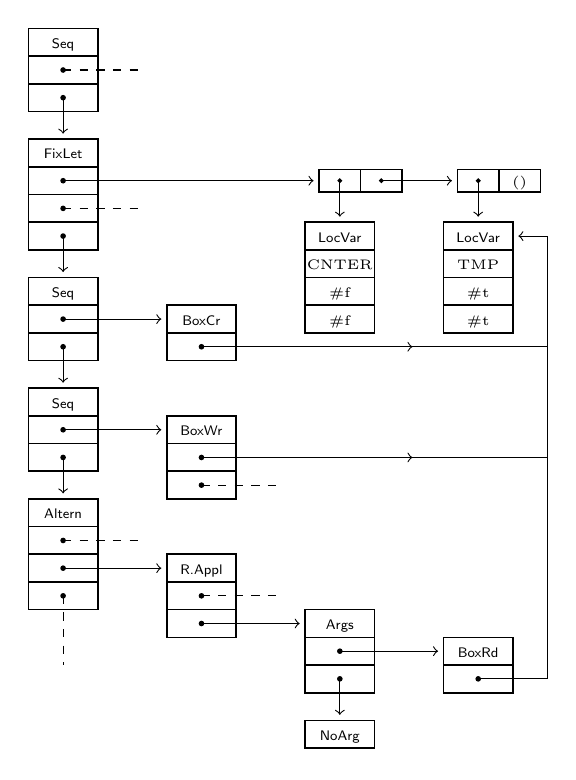
\begin{tikzpicture}
  \tikzstyle{every node}=[font=\tiny]

\def\NodeContent#1{\node [anchor = mid] at(1.25em, -0.5em) {#1};}
\def\NodeTitle#1{\NodeContent{\textsf{#1}}}
\def\NodePtr{\filldraw (1.25em, -0.5em) circle(0.8pt);}
\def\Box{\draw [semithick] (0, 0) rectangle (2.5em, -1.0em);}

\def\InList{%
  \begin{scope}[xshift = +0.5em, yshift = +1.5em]
    \draw [semithick] (0.0em, +0.4em) rectangle (3.0em, -0.4em)
                      (1.5em, +0.4em) -- (1.5em, -0.4em);
    \filldraw (0.75em, 0.0em) circle(0.65pt)
              (2.25em, 0.0em) circle(0.65pt);
  \end{scope}
}

\def\InListLast{%
  \begin{scope}[xshift = +0.5em, yshift = +1.5em]
    \draw [semithick] (0.0em, +0.4em) rectangle (3.0em, -0.4em)
                      (1.5em, +0.4em) -- (1.5em, -0.4em);
    \filldraw (0.75em, 0.0em) circle(0.65pt);
    \node [anchor = mid] at(2.25em, 0.0em) {\ic{()}};
  \end{scope}
}

\def\PullListLink{\draw [->] (-2.25em, 1.5em) -- (0.30em, 1.5em);}

\def\InBotList{%
  \begin{scope}[xshift = +0.5em, yshift = -1.5em]
    \draw [semithick] (0.0em, +0.4em) rectangle (3.0em, -0.4em)
                      (1.5em, +0.4em) -- (1.5em, -0.4em);
    \filldraw (0.75em, 0.0em) circle(0.65pt)
              (2.25em, 0.0em) circle(0.65pt);
  \end{scope}
}

\def\InBotListLast{%
  \begin{scope}[xshift = +0.5em, yshift = -1.5em]
    \draw [semithick] (0.0em, +0.4em) rectangle (3.0em, -0.4em)
                      (1.5em, +0.4em) -- (1.5em, -0.4em);
    \filldraw (0.75em, 0.0em) circle(0.65pt);
    \node [anchor = mid] at(2.25em, 0.0em) {\ic{()}};
  \end{scope}
}

\def\PullBotListLink{\draw [->] (-2.25em, -1.5em) -- (0.30em, -1.5em);}

\def\PullLinkUp{\draw    [->] ( 1.25em,  1.50em) -- ( 1.25em,  0.20em);}
\def\PullLinkLeft{\draw  [->] (-3.75em, -0.50em) -- (-0.20em, -0.50em);}
\def\PullLinkDown{\draw  [->] ( 1.25em, -1.50em) -- ( 1.25em, -0.20em);}
\def\PullLinkRight{\draw [->] ( 6.25em, -0.50em) -- ( 2.70em, -0.50em);}

\def\NoArgNode{%
  \begin{scope}[yshift = -0.0em]
    \Box
    \NodeTitle{NoArg}
  \end{scope}
}

\def\NoFreeNode{%
  \begin{scope}[yshift = -0.0em]
    \Box
    \NodeTitle{NoFree}
  \end{scope}
}

\def\PtrNodeU#1{%
  \begin{scope}[yshift = -0.0em]
    \Box
    \NodeTitle{#1}
  \end{scope}
  \begin{scope}[yshift = -1.0em]
    \Box
    \NodePtr
  \end{scope}
}

\def\ContentNode#1#2{
  \begin{scope}[yshift = -0.0em]
    \Box
    \NodeTitle{#1}
  \end{scope}
  \begin{scope}[yshift = -1.0em]
    \Box
    \NodeContent{#2}
  \end{scope}
}

\def\PtrNodeD#1{%
  \begin{scope}[yshift = -0.0em]
    \Box
    \NodeTitle{#1}
  \end{scope}
  \begin{scope}[yshift = -1.0em]
    \Box
    \NodePtr
  \end{scope}
  \begin{scope}[yshift = -2.0em]
    \Box
    \NodePtr
  \end{scope}
}

\def\ContentNodeD#1#2#3{
  \begin{scope}[yshift = -0.0em]
    \Box
    \NodeTitle{#1}
  \end{scope}
  \begin{scope}[yshift = -1.0em]
    \Box
    \NodeContent{#2}
  \end{scope}
  \begin{scope}[yshift = -2.0em]
    \Box
    \NodeContent{#3}
  \end{scope}
}

\def\PtrNodeDS#1{%
  \begin{scope}[yshift = -0.0em]
    \Box
    \NodeTitle{#1}
  \end{scope}
  \begin{scope}[yshift = -1.0em]
    \Box
    \begin{scope}[xshift = +0.35em]
      \NodePtr
    \end{scope}
  \end{scope}
  \begin{scope}[yshift = -2.0em]
    \Box
    \begin{scope}[xshift = -0.35em]
      \NodePtr
    \end{scope}
  \end{scope}
}

\def\PtrNodeT#1{
  \begin{scope}[yshift = -0.0em]
    \Box
    \NodeTitle{#1}
  \end{scope}
  \begin{scope}[yshift = -1.0em]
    \Box
    \NodePtr
  \end{scope}
  \begin{scope}[yshift = -2.0em]
    \Box
    \NodePtr
  \end{scope}
  \begin{scope}[yshift = -3.0em]
    \Box
    \NodePtr
  \end{scope}
}

\def\LocVarNode#1#2#3{
  \begin{scope}[yshift = -0.0em]
    \Box
    \NodeTitle{LocVar}
  \end{scope}
  \begin{scope}[yshift = -1.0em]
    \Box
    \NodeContent{#1}
  \end{scope}
  \begin{scope}[yshift = -2.0em]
    \Box
    \NodeContent{#2}
  \end{scope}
  \begin{scope}[yshift = -3.0em]
    \Box
    \NodeContent{#3}
  \end{scope}
}

\def\ClosureNode#1{
  \begin{scope}[yshift = -0.0em]
    \Box
    \NodeTitle{Closure}
  \end{scope}
  \begin{scope}[yshift = -1.0em]
    \Box
    \NodeContent{#1}
  \end{scope}
  \begin{scope}[yshift = -2.0em]
    \Box
    \NodePtr
  \end{scope}
  \begin{scope}[yshift = -3.0em]
    \Box
    \NodePtr
  \end{scope}
}

\def\FunDefNode#1{
  \begin{scope}[yshift = -0.0em]
    \Box
    \NodeTitle{FunDef}
  \end{scope}
  \begin{scope}[yshift = -1.0em]
    \Box
    \NodePtr
  \end{scope}
  \begin{scope}[yshift = -2.0em]
    \Box
    \NodePtr
  \end{scope}
  \begin{scope}[yshift = -3.0em]
    \Box
    \NodePtr
  \end{scope}
  \begin{scope}[yshift = -4.0em]
    \Box
    \NodeContent{#1}
  \end{scope}
}


\begin{scope}[xshift = 0.0em]
    \begin{scope}[yshift = -0.0em]
        \PtrNodeD{Seq}
    \begin{scope}[yshift = -4.0em]
        \PullLinkUp
        \PtrNodeT{FixLet}
    \begin{scope}[yshift = -5.0em]
        \PullLinkUp
        \PtrNodeD{Seq}
    \begin{scope}[yshift = -4.0em]
        \PullLinkUp
        \PtrNodeD{Seq}
    \begin{scope}[yshift = -4.0em]
        \PullLinkUp
        \PtrNodeT{Altern}
    \end{scope}\end{scope}\end{scope}
    \end{scope}\end{scope}
\end{scope}

% Seq ->
\draw [dashed] (1.25em,  -1.50em) -- (4.00em,  -1.50em);

% FixLet -> LocVarList
\draw [->] (1.25em, -5.50em) -- (10.30em, -5.50em);

% FixLet ->
\draw [dashed] (1.25em,  -6.50em) -- (4.00em,  -6.50em);

% Altern -> 
\draw [dashed] (1.25em, -18.50em) -- (4.00em, -18.50em);
\draw [dashed] (1.25em, -20.50em) -- (1.25em, -23.00em);

\begin{scope}[xshift = 5.0em]
    \begin{scope}[yshift = -10.0em]
        \PullLinkLeft
        \PtrNodeU{BoxCr}
    \begin{scope}[yshift = -4.0em]
        \PullLinkLeft
        \PtrNodeD{BoxWr}
    \begin{scope}[yshift = -5.0em]
        \PullLinkLeft
        \PtrNodeD{R.Appl}
    \end{scope}\end{scope}\end{scope}
\end{scope}

% BoxCr -> TMP
\draw [->] ( 6.25em, -11.50em) -- (13.875em, -11.50em);
\draw      (13.50em, -11.50em) -- (18.750em, -11.50em);

% BoxWr -> TMP
\draw [->] ( 6.25em, -15.50em) -- (13.875em, -15.50em);
\draw      (13.50em, -15.50em) -- (18.750em, -15.50em);

% BoxWr ->
\draw [dashed] (6.25em, -16.50em) -- (9.00em, -16.50em);

% R.Appl ->
\draw [dashed] (6.25em, -20.50em) -- (9.00em, -20.50em);

\begin{scope}[xshift = 10.0em]
    \begin{scope}[yshift =  -7.0em]
        \InList
        \PullLinkUp
        \LocVarNode{\ic{CNTER}}{\ic{\#f}}{\ic{\#f}}
    \begin{scope}[yshift = -14.0em]
        \PullLinkLeft
        \PtrNodeD{Args}
    \begin{scope}[yshift =  -4.0em]
        \PullLinkUp
        \NoArgNode
    \end{scope}\end{scope}\end{scope}
\end{scope}

\begin{scope}[xshift = 15.0em]
    \begin{scope}[yshift =  -7.0em]
        \InListLast
        \PullLinkUp
        \PullListLink
        \LocVarNode{\ic{TMP}}{\ic{\#t}}{\ic{\#t}}
    \begin{scope}[yshift = -15.0em]
        \PullLinkLeft
        \PtrNodeU{BoxRd}
    \end{scope}\end{scope}
\end{scope}

% BoxRd -> TMP
\draw [->] (16.25em, -23.50em) -- (18.75em, -23.50em) --
           (18.75em,  -7.50em) -- (17.70em,  -7.50em);

\end{tikzpicture}

\caption{\protect{\dc{(lambda (cnter~.~tmp) (set! tmp ...) (if ... (...~tmp) ...))}.}}%
\label{cc/boxes/pic:result}
\end{figure}


\section{Избавляемся от~вложенных~функций}\label{cc/sect:no-nest}

\indexR{функции!вложенные}
\indexR{лямбда-поднятие@$\lambda$-поднятие}
\indexE{lambda-lifting@$\lambda$-lifting}
\indexR{комбинаторы}
\indexR{свободные переменные}
\indexR{переменные!свободные}
Язык Си не~позволяет определять функции внутри других функций. Иными словами,
вложенные \ic{lambda}-формы нельзя прямо перевести на~Си. Следовательно, от них
необходимо избавиться, преобразовав программу в~набор комбинаторов "--- функций
без свободных переменных. К~счастью, это довольно известное преобразование,
называемое \term{$\lambda$"~поднятием} ($\lambda$"~lifting) "--- в~результате
него \ic{lambda}-формы поднимаются вверх, до самой поверхности, не~оставляя
ни~одной свободной переменной в~глубине программы. Существует множество
вариантов реализации подобного преобразования, по-разному обращающихся
с~исходными функциями и сохраняющих те или иные их аспекты, например:
\cite{ws94,kh89,ch94}.

\indexR{замыкания (closures)}
\indexC{invoke}
Результатом вычисления любой \ic{lambda}-формы является замыкание "--- сущность,
сохраняющая в~себе окружение, где она была создана. При вызове замыкания
специальная функция (известная как \ic{invoke}) берёт на себя работу по
организации вычисления тела данного замыкания в~правильном окружении,
составленном из аргументов функции, находящихся в~окружении вызова, и свободных
переменных, извлекаемых из замкнутого окружения. Фактически, это единственная
функция, которой известна истинная природа замыканий, поэтому мы можем довольно
легко изменить их структуру, не~потревожив остальные части программы: ведь
каждая аппликация в~конечном итоге выполняется \ic{invoke}.

\indexR{ОО-подъём}
\indexE{OO-lifting}
Рассмотрим упомянутое преобразование на примере \term{ОО-подъёма}, описанного
в~\cite{que94}. Как обычно, морской свинкой будет факториал:

\indexC{fact}
\begin{code:lisp}
(define (fact n k)
  (if (= n 0) (k 1)
      (fact (- n 1) (lambda (r) (k (* n r))) ) ) )
\end{code:lisp}

От \ic{lambda}-формы со~свободными переменными \ic{k} и~\ic{n} можно избавиться
следующим образом:

\begin{code:lisp}
(define-class Fact-Closure Object (n k))

(define-method (invoke (f Fact-Closure) r)
  (invoke (Fact-Closure-k f) (* (Fact-Closure-n f) r)) )

(define (fact n k)
  (if (= n 0) (invoke k 1)
      (fact (- n 1) (make-Fact-Closure n k)) ) )
\end{code:lisp}

\indexR{плоские окружения}
\indexR{окружение!плоское}
Суть преобразования состоит в~замене неявной структуры создаваемого анонимного
замыкания явным объектом класса \ic{Fact-Closure}, содержащим все необходимые
свободные переменные (здесь это \ic{n} и~\ic{k}). После этого остаётся только
научить \ic{invoke} корректным образом обрабатывать подобные объекты.

\indexR{преобразование!замыканий в~комбинаторы}
Для выполнения такого преобразования вначале надо как"~то получить и где"~то
сохранить список свободных переменных обрабатываемых функций. Для этого введём
новый класс преобразованных функций "--- \ic{Flat-Function}, а их свободные
переменные будем собирать в~списки из \ic{Free-Environment}, заканчивающиеся на
\ic{No-Free}. Как и их братья \ic{Arguments} и~\ic{No-Argument}, эти два класса
являются наследниками \ic{Program}, потому что представляют вычислимые понятия.
Обращения к~свободным переменным тоже будут преобразованы в~специальные объекты
класса \ic{Free-Reference}.

\ForLayout{display}{\begingroup
\lstset{aboveskip=\smallskipamount, belowskip=\smallskipamount}}

\indexC{Flat-Function}
\indexC{Free-Environment}
\indexC{Free-Reference}
\indexC{No-Free}
\begin{code:lisp}
(define-class Flat-Function    Function  (free))
(define-class Free-Environment Program   (first others))
(define-class No-Free          Program   ())
(define-class Free-Reference   Reference ())
\end{code:lisp}

Реализуется это преобразование, естественно, с~помощью обходчика кода. Функция
\ic{lift!} будет служить удобным интерфейсом, а всю чёрную работу мы переложим
на обобщённую функцию \ic{lift-procedures!}. Помимо обрабатываемой функции, она
принимает два вспомогательных аргумента: абстракцию \ic{flatfun}, которая
в~конечном итоге будет содержать все свободные переменные, и список \ic{vars},
где лежат все переменные, который на данный момент связаны. По умолчанию
\ic{lift-procedures!} просто рекурсивно вызывается для всех дочерних узлов
обрабатываемой программы.

\indexC{lift"!}
\indexC{lift-procedures"!}
\begin{code:lisp}
(define (lift! o)
  (lift-procedures! o #f '()) )

(define-generic (lift-procedures! (o Program) flatfun vars)
  (update-walk! lift-procedures! o flatfun vars) )
\end{code:lisp}

\ForLayout{display}{\endgroup}

Преобразование определяется всего тремя методами. Первый из них отвечает за
обработку обращений к~свободным переменным и поддержание списка \ic{flatfun}
в~адекватном состоянии. Функция \ic{adjoin-free-variable!} помогает с~занесением
новых свободных переменных в~этот список.

\indexC{adjoin-free-variable"!}
\begin{code:lisp}
(define-method (lift-procedures! (o Local-Reference) flatfun vars)
  (let ((v (Local-Reference-variable o)))
    (if (memq v vars) o
        (begin (adjoin-free-variable! flatfun o)
               (make-Free-Reference v) ) ) ) )

(define (adjoin-free-variable! flatfun ref)
  (when (Flat-Function? flatfun)
    (let check ((free* (Flat-Function-free flatfun)))
      (if (No-Free? free*)
          (set-Flat-Function-free!
           flatfun (make-Free-Environment
                    ref (Flat-Function-free flatfun) ) )
          (unless (eq? (Reference-variable ref)
                       (Reference-variable
                        (Free-Environment-first free*) ) )
            (check (Free-Environment-others free*)) ) ) ) ) )
\end{code:lisp}

\indexR{приводимые!формы}
\indexR{форма!приводимая}
Как известно, форма \ic{let} создаёт локальные привязки, поэтому перед
обработкой тела \ic{Fix-Let} необходимо поместить все свежесозданные связанные
переменные в~список \ic{vars}. Ещё одним неоспоримым фактом является то, что
приводимые формы, к~которым относится \ic{let}, лишь вводят новые переменные и
не~требуют создания замыканий. Это очень важная оптимизация, и мы отнюдь
не~хотим её лишиться.

\begin{code:lisp}
(define-method (lift-procedures! (o Fix-Let) flatfun vars)
  (set-Fix-Let-arguments!
   o (lift-procedures! (Fix-Let-arguments o) flatfun vars) )
  (let ((newvars (append (Fix-Let-variables o) vars)))
    (set-Fix-Let-body!
     o (lift-procedures! (Fix-Let-body o) flatfun newvars) )
    o ) )
\end{code:lisp}

Наконец, остался самый сложный случай "--- абстракции. Тело абстракции
анализируется и все её свободные переменные собираются в~объекте
\ic{Flat-Function}. Так как свободные переменные вложенной абстракции сами могут
оказаться свободными в~содержащей её абстракции, то для них обходчик вызывается
ещё раз, чтобы протолкнуть их как можно выше. Сейчас самое время порадоваться
принятому ранее решению сделать список свободных переменных наследником
\ic{Program}.

\begin{code:lisp}
(define-method (lift-procedures! (o Function) flatfun vars)
  (let* ((localvars (Function-variables o))
         (body      (Function-body o))
         (newfun (make-Flat-Function localvars body (make-No-Free))) )
    (set-Flat-Function-body!
     newfun (lift-procedures! body newfun localvars) )
    (let ((free* (Flat-Function-free newfun)))
      (set-Flat-Function-free!
       newfun (lift-procedures! free* flatfun vars) ) )
    newfun ) )
\end{code:lisp}

Как полагается, на рисунке~\ref{cc/no-nest/pic:result} показан результат
применения рассмотренного преобразования к~нашему бессменному примеру.

\begin{figure}\centering
% -*- coding: utf-8 -*-
% (lambda (i) (lambda x (cons i x)))
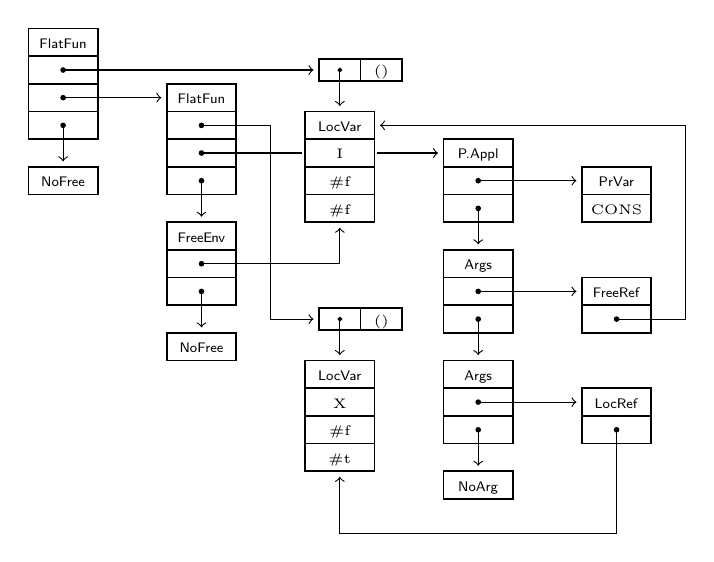
\begin{tikzpicture}
  \tikzstyle{every node}=[font=\tiny]

\def\NodeContent#1{\node [anchor = mid] at(1.25em, -0.5em) {#1};}
\def\NodeTitle#1{\NodeContent{\textsf{#1}}}
\def\NodePtr{\filldraw (1.25em, -0.5em) circle(0.8pt);}
\def\Box{\draw [semithick] (0, 0) rectangle (2.5em, -1.0em);}

\def\InList{%
  \begin{scope}[xshift = +0.5em, yshift = +1.5em]
    \draw [semithick] (0.0em, +0.4em) rectangle (3.0em, -0.4em)
                      (1.5em, +0.4em) -- (1.5em, -0.4em);
    \filldraw (0.75em, 0.0em) circle(0.65pt)
              (2.25em, 0.0em) circle(0.65pt);
  \end{scope}
}

\def\InListLast{%
  \begin{scope}[xshift = +0.5em, yshift = +1.5em]
    \draw [semithick] (0.0em, +0.4em) rectangle (3.0em, -0.4em)
                      (1.5em, +0.4em) -- (1.5em, -0.4em);
    \filldraw (0.75em, 0.0em) circle(0.65pt);
    \node [anchor = mid] at(2.25em, 0.0em) {\ic{()}};
  \end{scope}
}

\def\PullListLink{\draw [->] (-2.25em, 1.5em) -- (0.30em, 1.5em);}

\def\InBotList{%
  \begin{scope}[xshift = +0.5em, yshift = -1.5em]
    \draw [semithick] (0.0em, +0.4em) rectangle (3.0em, -0.4em)
                      (1.5em, +0.4em) -- (1.5em, -0.4em);
    \filldraw (0.75em, 0.0em) circle(0.65pt)
              (2.25em, 0.0em) circle(0.65pt);
  \end{scope}
}

\def\InBotListLast{%
  \begin{scope}[xshift = +0.5em, yshift = -1.5em]
    \draw [semithick] (0.0em, +0.4em) rectangle (3.0em, -0.4em)
                      (1.5em, +0.4em) -- (1.5em, -0.4em);
    \filldraw (0.75em, 0.0em) circle(0.65pt);
    \node [anchor = mid] at(2.25em, 0.0em) {\ic{()}};
  \end{scope}
}

\def\PullBotListLink{\draw [->] (-2.25em, -1.5em) -- (0.30em, -1.5em);}

\def\PullLinkUp{\draw    [->] ( 1.25em,  1.50em) -- ( 1.25em,  0.20em);}
\def\PullLinkLeft{\draw  [->] (-3.75em, -0.50em) -- (-0.20em, -0.50em);}
\def\PullLinkDown{\draw  [->] ( 1.25em, -1.50em) -- ( 1.25em, -0.20em);}
\def\PullLinkRight{\draw [->] ( 6.25em, -0.50em) -- ( 2.70em, -0.50em);}

\def\NoArgNode{%
  \begin{scope}[yshift = -0.0em]
    \Box
    \NodeTitle{NoArg}
  \end{scope}
}

\def\NoFreeNode{%
  \begin{scope}[yshift = -0.0em]
    \Box
    \NodeTitle{NoFree}
  \end{scope}
}

\def\PtrNodeU#1{%
  \begin{scope}[yshift = -0.0em]
    \Box
    \NodeTitle{#1}
  \end{scope}
  \begin{scope}[yshift = -1.0em]
    \Box
    \NodePtr
  \end{scope}
}

\def\ContentNode#1#2{
  \begin{scope}[yshift = -0.0em]
    \Box
    \NodeTitle{#1}
  \end{scope}
  \begin{scope}[yshift = -1.0em]
    \Box
    \NodeContent{#2}
  \end{scope}
}

\def\PtrNodeD#1{%
  \begin{scope}[yshift = -0.0em]
    \Box
    \NodeTitle{#1}
  \end{scope}
  \begin{scope}[yshift = -1.0em]
    \Box
    \NodePtr
  \end{scope}
  \begin{scope}[yshift = -2.0em]
    \Box
    \NodePtr
  \end{scope}
}

\def\ContentNodeD#1#2#3{
  \begin{scope}[yshift = -0.0em]
    \Box
    \NodeTitle{#1}
  \end{scope}
  \begin{scope}[yshift = -1.0em]
    \Box
    \NodeContent{#2}
  \end{scope}
  \begin{scope}[yshift = -2.0em]
    \Box
    \NodeContent{#3}
  \end{scope}
}

\def\PtrNodeDS#1{%
  \begin{scope}[yshift = -0.0em]
    \Box
    \NodeTitle{#1}
  \end{scope}
  \begin{scope}[yshift = -1.0em]
    \Box
    \begin{scope}[xshift = +0.35em]
      \NodePtr
    \end{scope}
  \end{scope}
  \begin{scope}[yshift = -2.0em]
    \Box
    \begin{scope}[xshift = -0.35em]
      \NodePtr
    \end{scope}
  \end{scope}
}

\def\PtrNodeT#1{
  \begin{scope}[yshift = -0.0em]
    \Box
    \NodeTitle{#1}
  \end{scope}
  \begin{scope}[yshift = -1.0em]
    \Box
    \NodePtr
  \end{scope}
  \begin{scope}[yshift = -2.0em]
    \Box
    \NodePtr
  \end{scope}
  \begin{scope}[yshift = -3.0em]
    \Box
    \NodePtr
  \end{scope}
}

\def\LocVarNode#1#2#3{
  \begin{scope}[yshift = -0.0em]
    \Box
    \NodeTitle{LocVar}
  \end{scope}
  \begin{scope}[yshift = -1.0em]
    \Box
    \NodeContent{#1}
  \end{scope}
  \begin{scope}[yshift = -2.0em]
    \Box
    \NodeContent{#2}
  \end{scope}
  \begin{scope}[yshift = -3.0em]
    \Box
    \NodeContent{#3}
  \end{scope}
}

\def\ClosureNode#1{
  \begin{scope}[yshift = -0.0em]
    \Box
    \NodeTitle{Closure}
  \end{scope}
  \begin{scope}[yshift = -1.0em]
    \Box
    \NodeContent{#1}
  \end{scope}
  \begin{scope}[yshift = -2.0em]
    \Box
    \NodePtr
  \end{scope}
  \begin{scope}[yshift = -3.0em]
    \Box
    \NodePtr
  \end{scope}
}

\def\FunDefNode#1{
  \begin{scope}[yshift = -0.0em]
    \Box
    \NodeTitle{FunDef}
  \end{scope}
  \begin{scope}[yshift = -1.0em]
    \Box
    \NodePtr
  \end{scope}
  \begin{scope}[yshift = -2.0em]
    \Box
    \NodePtr
  \end{scope}
  \begin{scope}[yshift = -3.0em]
    \Box
    \NodePtr
  \end{scope}
  \begin{scope}[yshift = -4.0em]
    \Box
    \NodeContent{#1}
  \end{scope}
}


\begin{scope}[xshift = 0.0em]
    \begin{scope}[yshift = -0.0em]
        \PtrNodeT{FlatFun}
    \begin{scope}[yshift = -5.0em]
        \PullLinkUp
        \NoFreeNode
    \end{scope}\end{scope}
\end{scope}

% FlatFun -> (LocVar : I)
\draw [->] (1.25em, -1.50em) -- (10.30em, -1.50em);

\begin{scope}[xshift = 5.0em]
    \begin{scope}[yshift = -2.0em]
        \PullLinkLeft
        \PtrNodeT{FlatFun}
    \begin{scope}[yshift = -5.0em]
        \PullLinkUp
        \PtrNodeD{Free{\kern-0.03em}E{\kern-0.04em}n{\kern-0.05em}v}
    \begin{scope}[yshift = -4.0em]
        \PullLinkUp
        \NoFreeNode
    \end{scope}\end{scope}\end{scope}
\end{scope}

% FlatFun -> (LocVar : X)
\draw [->] (6.25em,  -3.50em) -- ( 8.75em,  -3.50em) --
           (8.75em, -10.50em) -- (10.30em, -10.50em);

% FlatFun -> P.Appl
\draw      ( 6.25em,  -4.50em) -- ( 9.90em,  -4.50em);
\draw [->] (12.60em,  -4.50em) -- (14.80em,  -4.50em);

% FreeEnv -> LocVar : I
\draw [->] (6.25em, -8.50em) -- (11.25em, -8.50em) -- (11.25em, -7.20em);

\begin{scope}[xshift = 10.0em]
    \begin{scope}[yshift = -3.0em]
        \InListLast
        \PullLinkUp
        \LocVarNode{\ic{I}}{\ic{\#f}}{\ic{\#f}}
    \begin{scope}[yshift = -9.0em]
        \InListLast
        \PullLinkUp
        \LocVarNode{\ic{X}}{\ic{\#f}}{\ic{\#t}}
    \end{scope}\end{scope}
\end{scope}

\begin{scope}[xshift = 15.0em]
    \begin{scope}[yshift = -4.0em]
        \PtrNodeD{P.Appl}
    \begin{scope}[yshift = -4.0em]
        \PullLinkUp
        \PtrNodeD{Args}
    \begin{scope}[yshift = -4.0em]
        \PullLinkUp
        \PtrNodeD{Args}
    \begin{scope}[yshift = -4.0em]
        \PullLinkUp
        \NoArgNode
    \end{scope}\end{scope}\end{scope}
    \end{scope}
\end{scope}

\begin{scope}[xshift = 20.0em]
    \begin{scope}[yshift = -5.0em]
        \PullLinkLeft
        \ContentNode{PrVar}{\ic{CONS}}
    \begin{scope}[yshift = -4.0em]
        \PullLinkLeft
        \PtrNodeU{FreeRef}
    \begin{scope}[yshift = -4.0em]
        \PullLinkLeft
        \PtrNodeU{LocRef}
    \end{scope}\end{scope}\end{scope}
\end{scope}

% FreeRef -> LocVar : I
\draw [->] (21.25em, -10.50em) -- (23.75em, -10.50em) --
           (23.75em,  -3.50em) -- (12.70em,  -3.50em);

% LocRef -> LocVar : X
\draw [->] (21.25em, -14.50em) -- (21.25em, -18.25em) --
           (11.25em, -18.25em) -- (11.25em, -16.20em);
\end{tikzpicture}

\caption{\protect\dc{(lambda (i) (lambda x (cons i x)))}.}%
\label{cc/no-nest/pic:result}
\end{figure}


\section{Собираем цитаты и~функции}\label{cc/sect:collecting}

\indexR{миграция!цитат}
\indexR{миграция!вложенных функций}
Предыдущее преобразование не~изменяло расположения функций: вложенные
\ic{lambda}-формы так и остались вложенными, пусть и без свободных переменных.
Нет, мы не~забыли об~этом! Просто немного задержались, чтобы выполнить перенос
вместе со~следующим преобразованием "--- извлечением цитат. Во~время следующего
обхода кода мы извлечём все используемые цитаты и определения функций, чтобы
перенести их на глобальный уровень, как этого требует~Си. Здесь понадобятся
всего два метода.

Функция \ic{extract-things!} преобразовывает объекты \ic{Program} в~объекты
\ic{Flattened-Program}. Новый класс является наследником \ic{Program} и имеет
три дополнительных поля: \ic{form} для собственно программы, \ic{quotations} для
списка цитат и \ic{definitions} для определений функций. До значений цитат можно
добраться через глобальные переменные нового класса \ic{Quotation-Variable}.
Функции мы просто пронумеруем, выдав каждой из них уникальный \ic{index}.
Наконец, создание замыканий перекладывается на новый тип узлов синтаксического
дерева "--- \ic{Closure-Creation}. (Не~волнуйтесь, скоро вам станет ясно, почему
всё сделано именно так.)

\indexC{Flattened-Program}
\indexC{Quotation-Variable}
\indexC{Function-Definition}
\indexC{Closure-Creation}
\begin{code:lisp}
(define-class Flattened-Program   Program (form quotations definitions))
(define-class Quotation-Variable  Variable (value))
(define-class Function-Definition Flat-Function (index))
(define-class Closure-Creation    Program (index variables free))
\end{code:lisp}

Строго говоря, \ic{extract-things!} работает не~одна, а вместе с~обобщённой
функцией \ic{extract!}. Взаимодействие подразумевает обмен информацией. Дабы
не~прибегать для этого к~глобальным переменным (например, ради распараллеливания
компиляции), мы будем возвращать результат через специальный аргумент,
передаваемый обобщённой функции.

\indexC{extract-things}
\indexC{extract"!}
\begin{code:lisp}
(define (extract-things! o)
  (let ((result (make-Flattened-Program o '() '())))
    (set-Flattened-Program-form! result (extract! o result))
    result ) )

(define-generic (extract! (o Program) result)
  (update-walk! extract! o result) )
\end{code:lisp}

Цитаты просто собираются в~отведённом для них поле, а все обращения к~ним
заменяются обращениями к~соответствующим глобальным переменным,
инициализированным значениями исходных цитат.

\begin{code:lisp}
(define-method (extract! (o Constant) result)
  (let* ((qv* (Flattened-Program-quotations result))
         (qv  (make-Quotation-Variable (length qv*)
                                       (Constant-value o) )) )
    (set-Flattened-Program-quotations! result (cons qv qv*))
    (make-Global-Reference qv) ) )
\end{code:lisp}

Абстракции находятся в~узлах типа \ic{Flat-Function}, которые преобразуются
в~экземпляры \ic{Closure-Creation}. Процесс можно было~бы оптимизировать,
избежав дублирования кода для одинаковых абстракций, научив
\ic{adjoin-definition!} отыскивать повторения. Также может показаться странным,
что столько внимания уделяется спискам свободных переменных изначальных
абстракций. Это делается исключительно для облегчения определения арности
функций во~время генерации Си"~кода.

\indexC{adjoin-definition"!}
\begin{code:lisp}
(define-method (extract! (o Flat-Function) result)
  (let* ((newbody   (extract! (Flat-Function-body o) result))
         (variables (Flat-Function-variables o))
         (freevars  (let extract ((free (Flat-Function-free o)))
                      (if (Free-Environment? free)
                          (cons (Reference-variable
                                 (Free-Environment-first free) )
                                (extract
                                 (Free-Environment-others free) ) )
                          '() ) ))
         (index (adjoin-definition!
                 result variables newbody freevars )) )
    (make-Closure-Creation index variables (Flat-Function-free o)) ) )

(define (adjoin-definition! result variables body free)
  (let* ((definitions (Flattened-Program-definitions result))
         (newindex (length definitions)) )
    (set-Flattened-Program-definitions!
     result (cons (make-Function-Definition
                   variables body free newindex )
                  definitions ) )
    newindex ) )
\end{code:lisp}

И~снова, на рисунке~\ref{cc/collecting/pic:result} показан результат применения
преобразования к~иной части примера.

\begin{figure}\centering
% -*- coding: utf-8 -*-
% (begin (set! index 1) ((lambda ...) ... ))
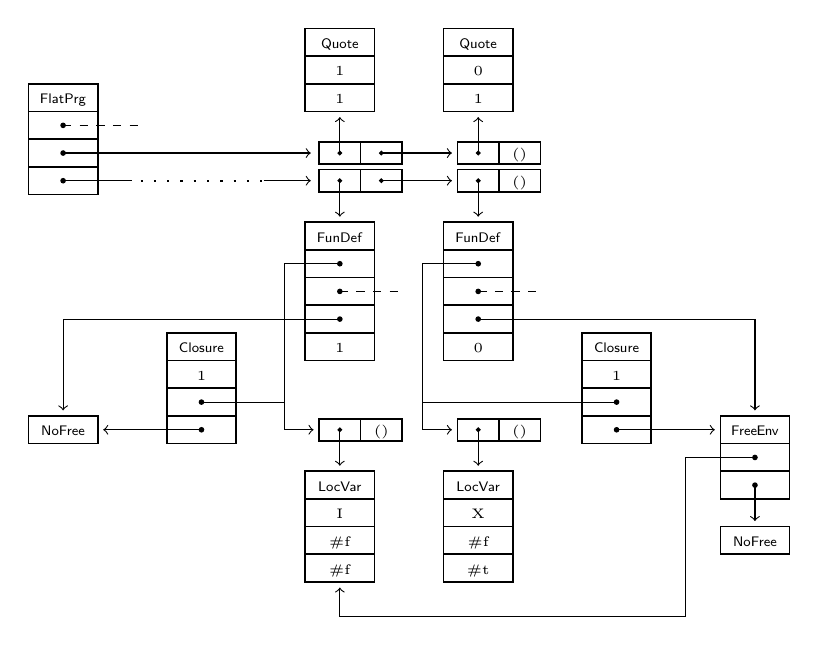
\begin{tikzpicture}
  \tikzstyle{every node}=[font=\tiny]

\def\NodeContent#1{\node [anchor = mid] at(1.25em, -0.5em) {#1};}
\def\NodeTitle#1{\NodeContent{\textsf{#1}}}
\def\NodePtr{\filldraw (1.25em, -0.5em) circle(0.8pt);}
\def\Box{\draw [semithick] (0, 0) rectangle (2.5em, -1.0em);}

\def\InList{%
  \begin{scope}[xshift = +0.5em, yshift = +1.5em]
    \draw [semithick] (0.0em, +0.4em) rectangle (3.0em, -0.4em)
                      (1.5em, +0.4em) -- (1.5em, -0.4em);
    \filldraw (0.75em, 0.0em) circle(0.65pt)
              (2.25em, 0.0em) circle(0.65pt);
  \end{scope}
}

\def\InListLast{%
  \begin{scope}[xshift = +0.5em, yshift = +1.5em]
    \draw [semithick] (0.0em, +0.4em) rectangle (3.0em, -0.4em)
                      (1.5em, +0.4em) -- (1.5em, -0.4em);
    \filldraw (0.75em, 0.0em) circle(0.65pt);
    \node [anchor = mid] at(2.25em, 0.0em) {\ic{()}};
  \end{scope}
}

\def\PullListLink{\draw [->] (-2.25em, 1.5em) -- (0.30em, 1.5em);}

\def\InBotList{%
  \begin{scope}[xshift = +0.5em, yshift = -1.5em]
    \draw [semithick] (0.0em, +0.4em) rectangle (3.0em, -0.4em)
                      (1.5em, +0.4em) -- (1.5em, -0.4em);
    \filldraw (0.75em, 0.0em) circle(0.65pt)
              (2.25em, 0.0em) circle(0.65pt);
  \end{scope}
}

\def\InBotListLast{%
  \begin{scope}[xshift = +0.5em, yshift = -1.5em]
    \draw [semithick] (0.0em, +0.4em) rectangle (3.0em, -0.4em)
                      (1.5em, +0.4em) -- (1.5em, -0.4em);
    \filldraw (0.75em, 0.0em) circle(0.65pt);
    \node [anchor = mid] at(2.25em, 0.0em) {\ic{()}};
  \end{scope}
}

\def\PullBotListLink{\draw [->] (-2.25em, -1.5em) -- (0.30em, -1.5em);}

\def\PullLinkUp{\draw    [->] ( 1.25em,  1.50em) -- ( 1.25em,  0.20em);}
\def\PullLinkLeft{\draw  [->] (-3.75em, -0.50em) -- (-0.20em, -0.50em);}
\def\PullLinkDown{\draw  [->] ( 1.25em, -1.50em) -- ( 1.25em, -0.20em);}
\def\PullLinkRight{\draw [->] ( 6.25em, -0.50em) -- ( 2.70em, -0.50em);}

\def\NoArgNode{%
  \begin{scope}[yshift = -0.0em]
    \Box
    \NodeTitle{NoArg}
  \end{scope}
}

\def\NoFreeNode{%
  \begin{scope}[yshift = -0.0em]
    \Box
    \NodeTitle{NoFree}
  \end{scope}
}

\def\PtrNodeU#1{%
  \begin{scope}[yshift = -0.0em]
    \Box
    \NodeTitle{#1}
  \end{scope}
  \begin{scope}[yshift = -1.0em]
    \Box
    \NodePtr
  \end{scope}
}

\def\ContentNode#1#2{
  \begin{scope}[yshift = -0.0em]
    \Box
    \NodeTitle{#1}
  \end{scope}
  \begin{scope}[yshift = -1.0em]
    \Box
    \NodeContent{#2}
  \end{scope}
}

\def\PtrNodeD#1{%
  \begin{scope}[yshift = -0.0em]
    \Box
    \NodeTitle{#1}
  \end{scope}
  \begin{scope}[yshift = -1.0em]
    \Box
    \NodePtr
  \end{scope}
  \begin{scope}[yshift = -2.0em]
    \Box
    \NodePtr
  \end{scope}
}

\def\ContentNodeD#1#2#3{
  \begin{scope}[yshift = -0.0em]
    \Box
    \NodeTitle{#1}
  \end{scope}
  \begin{scope}[yshift = -1.0em]
    \Box
    \NodeContent{#2}
  \end{scope}
  \begin{scope}[yshift = -2.0em]
    \Box
    \NodeContent{#3}
  \end{scope}
}

\def\PtrNodeDS#1{%
  \begin{scope}[yshift = -0.0em]
    \Box
    \NodeTitle{#1}
  \end{scope}
  \begin{scope}[yshift = -1.0em]
    \Box
    \begin{scope}[xshift = +0.35em]
      \NodePtr
    \end{scope}
  \end{scope}
  \begin{scope}[yshift = -2.0em]
    \Box
    \begin{scope}[xshift = -0.35em]
      \NodePtr
    \end{scope}
  \end{scope}
}

\def\PtrNodeT#1{
  \begin{scope}[yshift = -0.0em]
    \Box
    \NodeTitle{#1}
  \end{scope}
  \begin{scope}[yshift = -1.0em]
    \Box
    \NodePtr
  \end{scope}
  \begin{scope}[yshift = -2.0em]
    \Box
    \NodePtr
  \end{scope}
  \begin{scope}[yshift = -3.0em]
    \Box
    \NodePtr
  \end{scope}
}

\def\LocVarNode#1#2#3{
  \begin{scope}[yshift = -0.0em]
    \Box
    \NodeTitle{LocVar}
  \end{scope}
  \begin{scope}[yshift = -1.0em]
    \Box
    \NodeContent{#1}
  \end{scope}
  \begin{scope}[yshift = -2.0em]
    \Box
    \NodeContent{#2}
  \end{scope}
  \begin{scope}[yshift = -3.0em]
    \Box
    \NodeContent{#3}
  \end{scope}
}

\def\ClosureNode#1{
  \begin{scope}[yshift = -0.0em]
    \Box
    \NodeTitle{Closure}
  \end{scope}
  \begin{scope}[yshift = -1.0em]
    \Box
    \NodeContent{#1}
  \end{scope}
  \begin{scope}[yshift = -2.0em]
    \Box
    \NodePtr
  \end{scope}
  \begin{scope}[yshift = -3.0em]
    \Box
    \NodePtr
  \end{scope}
}

\def\FunDefNode#1{
  \begin{scope}[yshift = -0.0em]
    \Box
    \NodeTitle{FunDef}
  \end{scope}
  \begin{scope}[yshift = -1.0em]
    \Box
    \NodePtr
  \end{scope}
  \begin{scope}[yshift = -2.0em]
    \Box
    \NodePtr
  \end{scope}
  \begin{scope}[yshift = -3.0em]
    \Box
    \NodePtr
  \end{scope}
  \begin{scope}[yshift = -4.0em]
    \Box
    \NodeContent{#1}
  \end{scope}
}


\begin{scope}[xshift = 0.0em]
    \begin{scope}[yshift =  -0.0em]
        \PtrNodeT{FlatPrg}
    \begin{scope}[yshift = -12.0em]
        \NoFreeNode
        \PullLinkRight
    \end{scope}\end{scope}
\end{scope}

% FlagPrg ->
\draw [dashed] (1.25em, -1.50em) -- ( 4.00em, -1.50em);

% FlagPrg -> (Quote)
\draw [->]     (1.25em, -2.50em) -- (10.20em, -2.50em);

% FlagPrg -> (FunDef)
\draw                         (1.25em, -3.50em) -- ( 3.75em, -3.50em);
\draw [loosely dotted, thick] (4.05em, -3.50em) -- ( 8.45em, -3.50em);
\draw [->]                    (8.50em, -3.50em) -- (10.20em, -3.50em);

\begin{scope}[xshift = 5.0em]
    \begin{scope}[yshift = -9.0em]
        \ClosureNode{\ic{1}}
    \end{scope}
\end{scope}

\begin{scope}[xshift = 10.0em]
    \begin{scope}[yshift = +2.0em]
        \ContentNodeD{Quote}{\ic{1}}{\ic{1}}
        \begin{scope}[yshift = -3.0em]
            \InBotList
            \PullLinkDown
        \end{scope}
    \end{scope}
    \begin{scope}[yshift = -5.0em]
        \InList
        \PullLinkUp
        \FunDefNode{\ic{1}}
    \begin{scope}[yshift = -9.0em]
        \InListLast
        \PullLinkUp
        \LocVarNode{\ic{I}}{\ic{\#f}}{\ic{\#f}}
    \end{scope}\end{scope}
\end{scope}

% FunDef -> (LocVar : I)
% Closure -> (LocVar : I)
\draw [->] (11.25em,  -6.50em) -- ( 9.25em,  -6.50em) --
           ( 9.25em, -12.50em) -- (10.30em, -12.50em);
\draw      ( 6.25em, -11.50em) -- ( 9.25em, -11.50em);

% FunDef ->
\draw [dashed] (11.25em, -7.50em) -- (13.50em, -7.50em);

% FunDef -> NoFree
\draw [->] (11.25em, -8.50em) -- (1.25em, -8.50em) -- (1.25em, -11.80em);

\begin{scope}[xshift = 15.0em]
    \begin{scope}[yshift = +2.0em]
        \ContentNodeD{Quote}{\ic{0}}{\ic{1}}
        \begin{scope}[yshift = -3.0em]
            \InBotListLast
            \PullLinkDown
            \PullBotListLink
        \end{scope}
    \end{scope}
    \begin{scope}[yshift = -5.0em]
        \InListLast
        \PullLinkUp
        \PullListLink
        \FunDefNode{\ic{0}}
    \begin{scope}[yshift = -9.0em]
        \InListLast
        \PullLinkUp
        \LocVarNode{\ic{X}}{\ic{\#f}}{\ic{\#t}}
    \end{scope}\end{scope}
\end{scope}

% FunDef -> (LocVar : X)
% Closure -> (LocVar : X)
\draw [->] (16.25em,  -6.50em) -- (14.25em,  -6.50em) --
           (14.25em, -12.50em) -- (15.30em, -12.50em);
\draw      (21.25em, -11.50em) -- (14.25em, -11.50em);

% FunDef ->
\draw [dashed] (16.25em, -7.50em) -- (18.50em, -7.50em);

% FunDef -> FreeEnv
\draw [->] (16.25em, -8.50em) -- (26.25em, -8.50em) -- (26.25em, -11.80em);

\begin{scope}[xshift = 20.0em]
    \begin{scope}[yshift = -9.0em]
        \ClosureNode{\ic{1}}
    \end{scope}
\end{scope}

\begin{scope}[xshift = 25.0em]
    \begin{scope}[yshift = -12.0em]
        \PullLinkLeft
        \PtrNodeD{Free{\kern-0.03em}E{\kern-0.04em}n{\kern-0.05em}v}
    \begin{scope}[yshift =  -4.0em]
        \PullLinkUp
        \NoFreeNode
    \end{scope}\end{scope}
\end{scope}

% FreeEnv -> LocVar : I
\draw [->] (26.25em, -13.50em) -- (23.75em, -13.50em) -- (23.75em, -19.25em) --
           (11.25em, -19.25em) -- (11.25em, -18.20em);

\end{tikzpicture}

\caption{\protect\dc{(begin (set! index 1) ((lambda ...) ...~))}.}%
\label{cc/collecting/pic:result}
\end{figure}

\phantomlabel{cc/collecting/par:main}
Наконец, вся программа превращается в~вызов одной огромной функции. То~есть
$\pi$ становится \ic{((lambda~()~$\pi$))}.

\indexC{closurize-main"!}
\begin{code:lisp}
(define (closurize-main! o)
  (let ((index (length (Flattened-Program-definitions o))))
    (set-Flattened-Program-definitions!
     o (cons (make-Function-Definition
              '() (Flattened-Program-form o) '() index )
             (Flattened-Program-definitions o) ) )
    (set-Flattened-Program-form!
     o (make-Regular-Application
        (make-Closure-Creation index '() (make-No-Free))
        (make-No-Argument) ) )
    o ) )
\end{code:lisp}


\section{Собираем временные~переменные}\label{cc/sect:tmp}

У~автора всегда есть решительное преимущество перед читателем в~том, что он
знает, что хочет получить, а вы пока ещё не~знаете, что получится в~результате.
В~надежде на оригинальность, выражения Scheme было решено переводить
в~выражения~Си. Это выглядит немного эксцентричным, так как язык Си вообще"~то
построен вокруг инструкций (statements), а не~выражений (expressions), но такое
представление позволяет сохранить структуру Scheme в~получаемой на выходе
программе. Правда, в~этом случае возникает проблема с~переводом узлов типа
\ic{Fix-Let}, так как в~языке Си нельзя создавать локальные переменные внутри
выражений,\footnote*{Однако, например, \ic{gcc} расширяет язык формой
\ic{(\{~...~\})}, позволяющей вводить переменные где угодно.} только с~помощью
отдельных инструкций. Поэтому мы вынуждены будем пробежаться по всем
\ic{Fix-Let} и провести учёт всех локальных переменных, вводимых ими, чтобы
впоследствии корректно их объявить.

Естественно, для этого выполняется ещё один проход по коду. Задачей данного
прохода будет сбор всех локальных переменных форм \ic{Fix-Let} в~одном месте,
а также их переименование для предотвращения коллизий. Функции, имеющие
временные локальные переменные, мы будем представлять подклассом
\ic{Function-Definition}, называемым \ic{With-Temp-Function-Definition}.

\indexC{With-Temp-Function-Definition}
\begin{code:lisp}
(define-class With-Temp-Function-Definition Function-Definition
  ( temporaries ) )
\end{code:lisp}

Функция \ic{gather-temporaries!} реализует преобразование. Она полагается на
обобщённую функцию \ic{collect-temporaries!}, работающую в~паре с~обходчиком.
Вторым аргументом данной функции является объект, куда она будет складывать
обнаруженные переменные, а третий хранит список соответствий старых имён новым,
необходимый для выполнения переименований.

\indexC{gather-temporaries"!}
\indexC{collect-temporaries"!}
\begin{code:lisp}
(define (gather-temporaries! o)
  (set-Flattened-Program-definitions!
   o (map (lambda (def)
            (let ((flatfun (make-With-Temp-Function-Definition
                            (Function-Definition-variables def)
                            (Function-Definition-body def)
                            (Function-Definition-free def)
                            (Function-Definition-index def)
                            '() )))
              (collect-temporaries! flatfun flatfun '()) ) )
          (Flattened-Program-definitions o) ) )
  o )

(define-generic (collect-temporaries! (o Program) flatfun r)
  (update-walk! collect-temporaries! o flatfun r) )
\end{code:lisp}

Для завершения преобразования остаётся определить три новых метода. Локальные
переменные при необходимости могут переименовываться, то~же самое касается и
переменных в~коробках:

\begin{code:lisp}
(define-method (collect-temporaries! (o Local-Reference) flatfun r)
  (let* ((variable (Local-Reference-variable o))
         (v (assq variable r)) )
    (if (pair? v) (make-Local-Reference (cdr v))
                  o ) ) )

(define-method (collect-temporaries! (o Box-Creation) flatfun r)
  (let* ((variable (Box-Creation-variable o))
         (v (assq variable r)) )
    (if (pair? v) (make-Box-Creation (cdr v))
                  o ) ) )
\end{code:lisp}

Самый сложный метод, конечно~же, будет для \ic{Fix-Let}. Сначала он рекурсивно
вызывается для всех её аргументов, после чего переименовывает локальные
переменные с~помощью функции \ic{new-renamed-variable}. Затем эти новые
переменные добавляются в~определение обрабатываемой формы, а
\ic{collect-temporaries!} ещё раз рекурсивно вызывается уже для её тела,
помещённого в~обновлённое окружение.

\indexC{adjoin-temporary-variables"!}
\begin{code:lisp}
(define-method (collect-temporaries! (o Fix-Let) flatfun r)
  (set-Fix-Let-arguments!
   o (collect-temporaries! (Fix-Let-arguments o) flatfun r) )
  (let* ((newvars (map new-renamed-variable (Fix-Let-variables o)))
         (newr (append (map cons (Fix-Let-variables o) newvars) r)) )
    (adjoin-temporary-variables! flatfun newvars)
    (set-Fix-Let-variables! o newvars)
    (set-Fix-Let-body!
     o (collect-temporaries! (Fix-Let-body o) flatfun newr) )
    o ) )

(define (adjoin-temporary-variables! flatfun newvars)
  (let adjoin ((temps (With-Temp-Function-Definition-temporaries
                       flatfun ))
               (vars newvars) )
    (if (pair? vars)
        (if (memq (car vars) temps)
            (adjoin temps (cdr vars))
            (adjoin (cons (car vars) temps) (cdr vars)) )
        (set-With-Temp-Function-Definition-temporaries!
         flatfun temps ) ) ) )
\end{code:lisp}

Переименованные переменные выделяются в~собственный подкласс. Ещё нам
потребуется счётчик для обеспечения уникальности их имён.

\indexC{Renamed-Local-Variable}
\indexC{renaming-variable-counter}
\indexC{new-renamed-variable}
\begin{code:lisp}
(define-class Renamed-Local-Variable Variable (index))

(define renaming-variable-counter 0)

(define-generic (new-renamed-variable (variable)))

(define-method (new-renamed-variable (variable Local-Variable))
  (set! renaming-variable-counter (+ 1 renaming-variable-counter))
  (make-Renamed-Local-Variable
   (Variable-name variable) renaming-variable-counter ) )
\end{code:lisp}


\section{Передышка}\label{cc/sect:pause}

Следующая программа на Scheme является финальным результатом метаморфоз,
произошедших с~показанным в~самом начале главы примером. Итого:

\begin{enumerate}
  \item Изменяемые переменные разложены по коробками.
  \item Вложенные функции не~используются.
  \item Все цитаты и определения функций вынесены наверх.
  \item Временные переменные создаются явно.
\end{enumerate}

\begin{code:lisp}
(define quote_5 'foo)                    ; собранные цитаты
(define-class Closure_0 Object ())       ; абстракция \ic{(lambda~(f)~...)}
(define-method (invoke (self Closure_0) f)
  (begin
    (set! index (+ 1 index))
    (invoke f index) ) )                 ; вызов функции
(define-class Closure_1 Object (i))      ; абстракция \ic{(lambda~(x)~...)}
(define-method (invoke (self Closure_1) . x)
  (cons (Closure_1-i self)               ; свободная переменная~\ic{i}
        x ) )
(define-class Closure_2 Object ())       ; абстракция \ic{(lambda~(i)~...)}
(define-method (invoke (self Closure_2) i)
  (make-Closure_1 i) )                   ; создание замыкания
(define-class Closure_3 Object ())       ; абстракция \ic{(lambda~()~$\pi$)}
(define-method (invoke (self Closure_3))
  ((lambda (cnter_1 tmp_2)               ; переименование в~действии
     (set! index 1)
     (set! cnter_1 (make-Closure_0))     ; инициализация
     (set! tmp_2 (cons quote_5 '()))     ; \quad временных переменных
     (set! tmp_2 (make-box tmp_2))       ; укладываем в~коробку
     (box-write! tmp_2                   ; \quad изменяемую переменную
                 (invoke cnter_1 (make-Closure_2)) )
     (if cnter_1
         (invoke cnter_1 (box-read tmp_2))
         index ) ) ) )
(invoke (make-Closure_3))                ; точка входа
\end{code:lisp}


\section{Генерируем~Си}\label{cc/sect:gen}

Наконец, мы готовы выполнить мистический обряд кодогенерации. Осталось лишь
дать несколько предварительных пояснений. Ваш покорный слуга не~мнит себя
мировым экспертом по языку~Си и, в~сущности, обязан своими знаниями тщательному
изучению книг вроде \cite{iso90,hs91,cek+89}. Предполагается, что вы имеете
некоторое представление об~этом языке, но не~обременены предрассудками
о~единственно верном способе его использования.

Абстрактное синтаксическое дерево полностью готово и только и~ждёт, чтобы его 
скомпилировали, а~вернее сказать, \emph{распечатали} на языке~Си. Благодаря
высокоуровневому представлению программ, генерация кода не~представляет особых
сложностей. Функция \ic{compile->C} принимает S"=выражение, выполняет над ним
рассмотренные ранее преобразования и в~конце концов выводит в~порт \ic{out}
опрятный исходный код на~Си.

\indexC{compile->C}
\indexC{generate-C-program}
\begin{code:lisp}
(define (compile->C e out)
  (set! g.current '())
  (let ((prg (extract-things! (lift! (Sexp->object e)))))
    (gather-temporaries! (closurize-main! prg))
    (generate-C-program out e prg) ) )

(define (generate-C-program out e prg)
  (generate-header             out e)
  (generate-global-environment out g.current)
  (generate-quotations         out (Flattened-Program-quotations prg))
  (generate-functions          out (Flattened-Program-definitions prg))
  (generate-main               out (Flattened-Program-form prg))
  (generate-trailer            out)
  prg )
\end{code:lisp}

Как и любая программа на Си, а в~более широком смысле, как и любое животное,
получаемая программа состоит из головы, тела и~хвоста. В~голове находятся
желания, умения и мысли, поэтому там размещается комментарий с~исходным
выражением на Scheme (выводимым нестандартной функцией~\ic{pp}), а также
директива препроцессора, подключающая к~программе заголовочный файл
\ic{scheme.h}, где будут находиться все необходимые ей определения. Для вывода
строк программы здесь и далее используется ещё одна нестандартная функция
\ic{format}.

\indexC{generate-header}
\indexC{generate-trailer}
\begin{code:lisp}
(define (generate-header out e)
  (format out "/* Compiler to C $Revision: 4.1$~%")
  (pp e out)
  (format out "~%*/~%~%#include \"scheme.h\"~%") )

(define (generate-trailer out)
  (format out "~%/* End of generated code */~%") )
\end{code:lisp}

В~хвосте, как видите, нет ничего интересного; всё самое важное находится в~теле
программы. Результат компиляции нашего подопытного примера приведён на
странице~\pageref{cc/gen/init/src:result}. Возможно, вам захочется взглянуть на
него, прежде чем переходить к~изучению анатомии генератора.


\subsection{Глобальное окружение}\label{cc/gen/ssect:global}

Глобальные переменные, используемые программой, можно разделить на две группы:
предопределённые переменные, вроде \ic{car} или~\ic{+}, и изменяемые глобальные
переменные. Считается, что предопределённые переменные неизменяемы, а их
значения физически располагаются в~специальной библиотеке, которая будет
подключена при компоновке. В~отличие от них, окружение глобальных изменяемых
переменных должно быть сформировано именно у~нас в~программе. Для этого мы
используем информацию, которую собрали в~\ic{g.current} во~время предобработки.

Используемый подход к~генерации строится на предположении, что программа
компилируется целиком, а не~отдельными модулями. (Раздельная компиляция, как
вы помните, вызывает множество специфичных затруднений.
\seePage[compilation/sect:separate] Мы не~будем их рассматривать повторно, дабы
не~раздувать эту главу в~пару~раз.)

Для облегчения понимания и повышения читабельности кода, генератор щедро
использует макросы~Си. Например, глобальные переменные объявляются макросом
\ic{SCM\_DefineGlobalVariable}. Вторым аргументом этот макрос принимает строку
с~изначальным именем\footnote{Используемая в~этой главе функция \ic{read}
переводит все имена символов в~верхний регистр.} переменной на Scheme. Это может
оказаться полезным при отладке.

\indexC{generate-global-environment}
\indexC{generate-global-variable}
\begin{code:lisp}
(define (generate-global-environment out gv*)
  (when (pair? gv*)
    (format out "~%/* Global environment: */~%")
    (for-each (lambda (gv) (generate-global-variable out gv))
              gv* ) ) )

(define (generate-global-variable out gv)
  (let ((name (Global-Variable-name gv)))
    (format out "SCM_DefineGlobalVariable(~A,\"~A\");~%"
            (IdScheme->IdC name) name ) ) )
\end{code:lisp}

\indexR{идентификаторы в~Си}
Вот мы и встретились с~первым затруднением: не~все идентификаторы Scheme
являются допустимыми в~Си. Функция \ic{IdScheme->IdC} занимается преобразованием
идентификаторов Scheme в~корректные идентификаторы~Си. Она должна избавиться от
всех мешающих символов, оставив при этом имя более-менее понятным, чтобы можно
было догадаться о~его исходном написании. Естественно, вариантов такого
преобразования огромное множество, но мы просто заменим все недопустимые символы
допустимыми, после чего убедимся в~уникальности полученного имени. Код, который
это делает, не~то, чтобы особо интересен, но в~самом начале книги у~нас был
уговор: ничего не~утаивать. Переменная \ic{Scheme->C-names-mapping} хранит
словарик имён, изначально содержащий несколько сложных случаев.

\indexC{IdScheme->IdC}
\begin{code:lisp}
(define Scheme->C-names-mapping
  '( (*        . "TIMES")
     (<        . "LESSP")
     (pair?    . "CONSP")
     (set-cdr! . "RPLACD")
     ; и другие
     ) )
(define (IdScheme->IdC name)
  (let ((v (assq name Scheme->C-names-mapping)))
    (if (pair? v) (cdr v)
        (let ((str (symbol->string name)))
          (let retry ((Cname (compute-Cname str)))
            (if (Cname-clash? Cname Scheme->C-names-mapping)
                (retry (compute-another-Cname str))
                (begin (set! Scheme->C-names-mapping
                             (cons (cons name Cname)
                                   Scheme->C-names-mapping ) )
                       Cname ) ) ) ) ) ) )
\end{code:lisp}

Обнаруженные конфликты имён разрешаются просто: добавлением уникального номера.

\ForLayout{display}{\begingroup\lstset{belowskip=\smallskipamount}}

\indexC{Cname-clash?}
\indexC{compute-Cname}
\begin{code:lisp}
(define (Cname-clash? Cname mapping)
  (let check ((mapping mapping))
    (and (pair? mapping)
         (or (string=? Cname (cdar mapping))
             (check (cdr mapping)) ) ) ) )

(define compute-another-Cname
  (let ((counter 1))
    (lambda (str)
      (set! counter (+ 1 counter))
      (compute-Cname (format #f "~A_~A" str counter)) ) ) )

(define (compute-Cname str)
  (define (mapcan f l)
    (if (not (pair? l)) '()
        (append (f (car l)) (mapcan f (cdr l))) ) )
  (define (convert-char char)
    (case char
      ((#\_)             '(#\_ #\_))
      ((#\?)             '(#\p))
      ((#\!)             '(#\i))
      ((#\<)             '(#\l))
      ((#\>)             '(#\g))
      ((#\=)             '(#\e))
      ((#\- #\/ #\* #\:) '())
      (else              (list char)) ) )
  (let ((cname (mapcan convert-char (string->list str))))
    (if (pair? cname)
        (list->string cname)
        "weird" ) ) )
\end{code:lisp}

\ForLayout{display}{\endgroup}

Единичные подчёркивания гарантированно не~встречаются в~генерируемых именах,
поэтому их можно спокойно использовать для именования разнообразных внутренних
переменных, не~опасаясь коллизий с~переменными исходной программы. Рассмотренное
преобразование, конечно, не~справится с~чем"~то вроде~\ic{1+}, но кого волнуют
имена, запрещённые стандартом Scheme?


\subsection{Цитаты}\label{cc/gen/ssect:quote}

\indexR{цитаты!склеивание}
\indexR{склеивание цитат}
Цитаты должны переводиться в~структуры данных Си, чтобы ими можно было
пользоваться в~программе. Мы поступим рационально, переводя их сразу в~готовые
определения структур данных, а не~в~код, который их создаст во~время исполнения.
Также мы оптимизируем занимаемый цитатами объём памяти, выделив в~них и
определив отдельно все общие подвыражения.

Функция \ic{generate-quotations} назначена ответственной за выполнение данных
обещаний. Для простоты мы не~будем реализовывать поддержку векторов, длинной
арифметики и~всех нецелых чисел.

\indexC{generate-quotations}
\begin{code:lisp}
(define (generate-quotations out qv*)
  (when (pair? qv*)
    (format out "~%/* Quotations: */~%")
    (scan-quotations out qv* (length qv*) '()) ) )
\end{code:lisp}

Настоящую работу выполняет \ic{scan-quotations}: просматривает собранные
цитаты, представляемые объектами класса \ic{Quotation-Variable}, и генерирует
соответствующий код. Она также старается создавать как можно меньше
промежуточных цитат, разделяя максимум информации между ними. Предикат
\ic{already-seen-value?} подсказывает ей, когда такое возможно.

\indexC{scan-quotations}
\indexC{already-seen-value"?}
\begin{code:lisp}
(define (scan-quotations out qv* i results)
  (when (pair? qv*)
    (let* ((qv       (car qv*))
           (value    (Quotation-Variable-value qv))
           (other-qv (already-seen-value? value results)) )
      (cond
        (other-qv
          (generate-quotation-alias out qv other-qv)
          (scan-quotations out (cdr qv*) i (cons qv results)) )
        ((C-value? value)
          (generate-C-value out qv)
          (scan-quotations out (cdr qv*) i (cons qv results)) )
        ((symbol? value) (scan-symbol out value qv* i results) )
        ((pair? value)   (scan-pair out value qv* i results) )
        (else (generate-error "Unsupported constant" qv)) ) ) ) )

(define (already-seen-value? value qv*)
  (and (pair? qv*)
       (if (equal? value (Quotation-Variable-value (car qv*)))
           (car qv*)
           (already-seen-value? value (cdr qv*)) ) ) )
\end{code:lisp}

Имена всех цитат в~генерируемом коде будут начинаться на~\ic{thing}. Если
в~программе нашлась пара эквивалентных цитат, то достаточно одну из них везде
заменить другой. Функция \ic{generate-quotation-alias} перекладывает эту работу
на препроцессор~Си. Чтобы облегчить чтение сгенерированного кода, рядом
помещается комментарий со~значением цитаты.

\indexC{generate-quotation-alias}
\begin{code:lisp}
(define (generate-quotation-alias out qv1 qv2)
  (format out "#define thing~A thing~A /* ~S */~%"
          (Quotation-Variable-name qv1)
          (Quotation-Variable-name qv2)
          (Quotation-Variable-value qv2) ) )
\end{code:lisp}

\indexR{значения!атомарные}
Предикат \ic{C-value?} проверяет, можно~ли данную цитату прямо перевести на~Си.
Если да, то она передаётся функции \ic{generate-C-value}, чтобы она выполнила
этот перевод. Непосредственными значениями являются пустой список, булевы
значения, (короткие) целые числа и~строки. Все эти значения Scheme можно сразу
представить соответствующими значениями~Си. Предположим на время, что у~нас уже
есть необходимые макросы, раскрывающиеся в~правильные описания строк, чисел,
истины, лжи и пустого списка. Все они начинаются на \ic{SCM\_}. Без сомнения,
гуру~Си также заметят, что наши числа являются знаковыми 31"~битными
в~дополнительном коде.

\indexC{C-value?}
\indexC{generate-C-value}
\begin{code:lisp}
(define *maximal-fixnum* +1073741823)
(define *minimal-fixnum* -1073741824)
|\ForLayout{display}{\vskip-0.333\baselineskip}|
(define (C-value? value)
  (or (null? value)
      (boolean? value)
      (and (integer? value)
           (<= *minimal-fixnum* value *maximal-fixnum*) )
      (string? value) ) )
|\ForLayout{display}{\vskip-0.333\baselineskip}|
(define (generate-C-value out qv)
  (let ((value (Quotation-Variable-value qv))
        (index (Quotation-Variable-name qv)) )
    (cond
      ((null? value)
        (format out "#define thing~A SCM_nil /* () */~%"
                index ) )
      ((boolean? value)
        (format out "#define thing~A ~A /* ~S */~%"
                index (if value "SCM_true" "SCM_false") value ) )
      ((integer? value)
        (format out "#define thing~A SCM_Int2Fixnum(~A)~%"
                index value ) )
      ((string? value)
        (format out "SCM_DefineString(thing~A_object, \"~A\");~%"
                index value )
        (format out "#define thing~A SCM_Wrap(&thing~A_object)~%"
                index index ) ) ) ) )
\end{code:lisp}

\indexR{значения!составные}
Если цитируются составные значения (точечные пары или символы), то вначале они
разбиваются на части, чтобы по возможности повторно использовать предыдущие
определения. Символы состоят из знаков, образующих строку с~их именем. Строки
создаются перед символами.

\indexC{scan-symbol}
\indexC{generate-symbol}
\begin{code:lisp}
(define (scan-symbol out value qv* i results)
  (let* ((qv (car qv*))
         (str (symbol->string value))
         (strqv (already-seen-value? str results)) )
    (cond (strqv
            (generate-symbol out qv strqv)
            (scan-quotations out (cdr qv*) i (cons qv results)) )
          (else
            (let ((newqv (make-Quotation-Variable i str)))
              (scan-quotations out (cons newqv qv*)
                               (+ i 1) results ) ) ) ) ) )

(define (generate-symbol out qv strqv)
  (format out "SCM_DefineSymbol(thing~A_object, thing~A); /* ~S */~%"
          (Quotation-Variable-name qv)
          (Quotation-Variable-name strqv)
          (Quotation-Variable-value qv) )
  (format out "#define thing~A SCM_Wrap(&thing~A_object)~%"
          (Quotation-Variable-name qv)
          (Quotation-Variable-name qv) ) )
\end{code:lisp}

Точечные пары состоят из двух частей "--- \ic{car} и~\ic{cdr}, "---
обрабатываемых последовательно. При этом учитывается, что их значения могут
оказаться эквивалентными как ранее определённым цитатам, так и друг другу. Их
вывод реализован в~стиле передачи продолжений.

\indexC{scan-pair}
\indexC{generate-pair}
\begin{code:lisp}
(define (scan-pair out value qv* i results)
  (let* ((qv  (car qv*))
         (d   (cdr value))
         (dqv (already-seen-value? d results)) )
    (if dqv
        (let* ((a   (car value))
               (aqv (already-seen-value? a results)) )
          (if aqv
              (begin
                (generate-pair out qv aqv dqv)
                (scan-quotations out (cdr qv*)
                                 i (cons qv results) ) )
              (let ((newaqv (make-Quotation-Variable i a)))
                (scan-quotations out (cons newaqv qv*)
                                 (+ i 1) results ) ) ) )
        (let ((newdqv (make-Quotation-Variable i d)))
          (scan-quotations
           out (cons newdqv qv*) (+ i 1) results ) ) ) ) )

(define (generate-pair out qv aqv dqv)
  (format out
          "SCM_DefinePair(thing~A_object, thing~A, thing~A); /* ~S */~%"
          (Quotation-Variable-name qv)
          (Quotation-Variable-name aqv)
          (Quotation-Variable-name dqv)
          (Quotation-Variable-value qv) )
  (format out
          "#define thing~A SCM_Wrap(&thing~A_object)~%"
          (Quotation-Variable-name qv)
          (Quotation-Variable-name qv) ) )
\end{code:lisp}

Теперь давайте рассмотрим пример, а затем поговорим обо~всех этих загадочных
макросах.


\subsection{Объявление данных}\label{cc/gen/ssect:decl}

Возьмём простую программу, состоящую из единственной цитаты: \ic{(quote ((\#F
\#T) (FOO . "FOO") 33 FOO . "FOO"))}. Её компиляция выдаёт следующий результат,
слегка приправленный комментариями. Наслаждайтесь!

% Такое разнообразие хешиков (\#, #) -- следствие абсолютно невразумительной
% обработки комментариев пакетом lstlistings. Где-то внутри комментариев
% горизонтальный режим, где-то -- verbatim-режим, в котором команды не работают.
% Я нифига не понял этих свистоплясок с наличием/отсутствием скобочек и пробелов
% и тупо всё захардкодил, чтобы выглядело нормально.
\begin{code:c-frame}
/* Compiler to C $Revision: 4.1$
'((#F #T) (FOO . "FOO") 33 FOO . "FOO") */

#include "scheme.h"

/* Quotations: */
SCM_DefineString(thing4_object, "FOO");
#define thing4 SCM_Wrap(&thing4_object)
SCM_DefineSymbol(thing5_object, thing4);        /* FOO */
#define thing5 SCM_Wrap(&thing5_object)
SCM_DefinePair(thing3_object, thing5, thing4);  /* (FOO . "FOO") */
#define thing3 SCM_Wrap(&thing3_object)
#define thing6 SCM_Int2Fixnum(33)
SCM_DefinePair(thing2_object, thing6, thing3);  /* (33 FOO . "FOO") */
#define thing2 SCM_Wrap(&thing2_object)
SCM_DefinePair(thing1_object, thing3, thing2);
                                  /* ((FOO . "FOO") 33 FOO . "FOO") */
#define thing1 SCM_Wrap(&thing1_object)
#define thing9 SCM_nil                           /* ()  */
#define thing10 SCM_true                         /* \#T  */
SCM_DefinePair(thing8_object, thing10, thing9);  /* (#T) */
#define thing8 SCM_Wrap(&thing8_object)
#define thing11 SCM_false                        /* \#F */
SCM_DefinePair(thing7_object, thing11, thing8);  /* (#F #T) */
#define thing7 SCM_Wrap(&thing7_object)
SCM_DefinePair(thing0_object, thing7, thing1);
                          /* ((#F #T) (FOO . "FOO") 33 FOO . "FOO") */
#define thing0 SCM_Wrap(&thing0_object)

/* ... */
\end{code:c-frame}

Первым делом создаётся строка \ic{"FOO"}. Для этого используется макрос
\ic{SCM\_DefineString}. Первым аргументом он принимает имя нового объекта на~Си.
Вторым "--- собственно строку. Похожим образом с~помощью макроса
\ic{SCM\_DefineSymbol} создаётся символ. Первым аргументом идёт имя на~Cи, за
ним "--- строка с~именем на Scheme. Точечные пары создаются аналогично с~помощью
макроса \ic{SCM\_DefinePair}: первым аргументом "--- имя на~Си, вторым и третьим
"--- содержимое \ic{car} и~\ic{cdr} соответственно.

Предопределённые объекты вроде булевых значений и пустого списка, конечно~же,
не~создаются каждый раз заново. Вместо этого используются напрямую их имена:
\ic{SCM\_true}, \ic{SCM\_false} и~\ic{SCM\_nil}.

Позже \seePage[cc/sect:data] мы подробнее разберём представление в~памяти
значений Scheme. Процесс компиляции слабо связан с~используемой конкретной
реализацией структур данных. На данный момент достаточно знать лишь её
интерфейс: объекты инициализируются директивами вида \ic{SCM\_Define...}, а
ссылку на инициализированный объект можно получить с~помощью \ic{SCM\_Wrap}.
Целые числа преобразуются в~объекты Scheme макросом \ic{SCM\_Int2Fixnum}.
К~любому объекту можно обратиться, использовав его имя, начинающееся на
\ic{thing}. Например, \ic{thing4} означает строку \ic{"FOO"}, а \ic{thing6} "---
это число~33. Точнее, \ic{thing4} "--- это указатель на объект
\ic{thing4\_object}, который уже хранит настоящую строку.

Строка \ic{"FOO"} общая для всех объектов: в~выражении \ic{(FOO . "FOO")}
объекты \ic{thing4} и \ic{thing3} ссылаются на один и тот~же
\ic{thing4\_object}.


\subsection{Компиляция выражений}\label{cc/gen/ssect:exprs}

Главной задачей компилятора, конечно~же, является перевод выражений Scheme
в~выражения~Си. Как было сказано ранее, мы намеренно преобразуем выражения
в~аналогичные выражения, а не~наборы инструкций с~тем~же смыслом. Поступив так,
мы определённо получим на выходе более понятный код, в~котором будет лучше видна
структура исходной программы. Однако, несмотря на очевидную мудрость подобного
решения, оно поднимает пару непростых вопросов, так как идёт вразрез
с~философией языка~Си. В~Си отдельные инструкции предпочтительнее выражений.
Не~то, чтобы это было особой проблемой для компилятора "--- ему"~то без разницы;
это будет проблемой для человека, который сядет отлаживать подобную программу.
Беда в~том, что интерактивные отладчики вроде \ic{gdb} обычно понимают пошаговый
режим исполнения как исполнение программы по инструкциям "--- а инструкции
в~нашем случае будут отнюдь не~маленькие. Если~бы мы решили компилировать Scheme
в~инструкции~Си вместо выражений, то в~итоге у~нас получилось~бы нечто похожее
на рассмотренный ранее компилятор в~байт"~код. \seePage[chapter:compilation]

Компиляция выражений выполняется обобщённой функцией~\ic{"~>C}. Она принимает
два аргумента: исходное выражение и порт, куда следует записать результат. Так
как результат компиляции сразу~же переносится в~файл, то код необходимо
генерировать строго последовательно, без возвратов и исправлений задним числом,
за один проход.
\seePage[compilation/lang-and-target/par:backtracking]

\indexC*{c}{->C}
\begin{code:lisp}
(define-generic (->C (e Program) out))
\end{code:lisp}

В~отличие от предыдущих трансформаций, в~этот раз мы не~будем использовать
обобщённый обходчик (так как у~нас нет действия по умолчанию), а просто
перечислим методы обработки каждого типа узлов синтаксического дерева. Эти
методы довольно просты по своей структуре, так как им надо лишь правильно
выводить соответствующие инструкции~Си.

Язык~Си имеет весьма строгий синтаксис с~чётко прописанными приоритетами,
ассоциативностью операций {\itd} Эти правила мало кто из программистов помнит
наизусть целиком, поэтому при малейших сомнениях все пользуются скобками. Мы~же
возведём эту практику в~абсолют и будем ставить их всегда. Что~бы там
ни~говорили сишники о~плохом вкусе, но исходным языком сейчас является Лисп,
так что в~программе должны быть скобочки. Много скобочек. Поэтому мы определим
специальный макрос, чтобы удобно их ставить:

\indexC{between-parentheses}
\begin{code:lisp}
(define-syntax between-parentheses
  (syntax-rules ()
    ((between-parentheses out . body)
     (let ((out out))
       (format out "(")
       (begin . body)
       (format out ")") ) ) ) )
\end{code:lisp}


\subsubsection{Обращения к~переменным}\label{cc/gen/exprs/sssect:refs}

В~программе могут использоваться переменные разного вида, но в~общем случае
одна переменная Scheme соответствует одной переменной~Си. Метод обработки
обращений к~переменным сразу~же перепоручает всю работу обобщённой функции
\ic{reference->C}, а она, в~свою очередь, по умолчанию просит всё сделать
следующую функцию "--- \ic{variable->C}. Такая слабая связанность методов
облегчит их дальнейшую специализацию.

\indexCS*{c}{->C}{\ic{Reference}}
\indexC{reference->C}
\indexC{variable->C}
\begin{code:lisp}
(define-method (->C (e Reference) out)
  (reference->C (Reference-variable e) out) )

(define-generic (reference->C (v Variable) out)
  (variable->C v out) )

(define-generic (variable->C (variable) out))
\end{code:lisp}

Обычно переменная получает новое имя на Си, похожее на её исходное, за
исключением случаев, когда она была переименована или~же ссылается на цитату.

\begin{code:lisp}
(define-method (variable->C (variable Variable) out)
  (format out (IdScheme->IdC (Variable-name variable))) )

(define-method (variable->C (variable Renamed-Local-Variable) out)
  (format out "~A_~A"
          (IdScheme->IdC (Variable-name variable))
          (Renamed-Local-Variable-index variable) ) )

(define-method (variable->C (variable Quotation-Variable) out)
  (format out "thing~A" (Quotation-Variable-name variable)) )
\end{code:lisp}

Отдельно обрабатываются обращения к~глобальным переменным, не~являющимся
предопределёнными. Фактически, это свободные переменные всей программы. Как вы
помните, в~данной реализации подобные переменные создаются автоматически, при их
первом упоминании. К~сожалению, компилятор никак не~анализирует значения этих
переменных, поэтому проверки на инициализированность должны проводиться во~время
исполнения программы. За этим проследит макрос \ic{SCM\_CheckedGlobal}.
\seeEx[cc/ex:global-check]

\begin{code:lisp}
(define-method (reference->C (v Global-Variable) out)
  (format out "SCM_CheckedGlobal")
  (between-parentheses out
    (variable->C v out) ) )
\end{code:lisp}

Кроме того, ещё остаются обычные свободные переменные. Для них тоже припасён
специальный макрос.

\indexCS*{c}{->C}{\ic{Free-Reference}}
\begin{code:lisp}
(define-method (->C (e Free-Reference) out)
  (format out "SCM_Free")
  (between-parentheses out
    (variable->C (Free-Reference-variable e) out) ) )
\end{code:lisp}


\subsubsection{Присваивания}\label{cc/gen/exprs/sssect:assignments}

С~присваиваниями всё ещё легче, так как они бывают лишь двух видов: присваивание
глобальным переменным и модификация содержимого коробок. Случай глобальных
переменных прямо переводится в~присваивание соответствующей глобальной
переменной языка~Си.

\indexCS*{c}{->C}{\ic{Global-Assignment}}
\begin{code:lisp}
(define-method (->C (e Global-Assignment) out)
  (between-parentheses out
    (variable->C (Global-Assignment-variable e) out)
    (format out " = ")
    (->C (Global-Assignment-form e) out) ) )
\end{code:lisp}


\subsubsection{Коробки}\label{cc/gen/exprs/sssect:boxes}

Что касается коробок, то над ними возможны всего три операции. Макрос
\ic{SCM\_Content} позволяет смотреть или изменять содержимое коробок, а
библиотечная функция \ic{SCM\_allocate\_box} берёт на себя их создание.

\indexCS*{c}{->C}{\ic{Box-Read}}
\indexCS*{c}{->C}{\ic{Box-Write}}
\indexCS*{c}{->C}{\ic{Box-Creation}}
\begin{code:lisp}
(define-method (->C (e Box-Read) out)
  (format out "SCM_Content")
  (between-parentheses out
    (->C (Box-Read-reference e) out) ) )

(define-method (->C (e Box-Write) out)
  (between-parentheses out
    (format out "SCM_Content")
    (between-parentheses out
      (->C (Box-Write-reference e) out) )
    (format out " = ")
    (->C (Box-Write-form e) out) ) )

(define-method (->C (e Box-Creation) out)
  (variable->C (Box-Creation-variable e) out)
  (format out " = SCM_allocate_box")
  (between-parentheses out
    (variable->C (Box-Creation-variable ) out) ) )
\end{code:lisp}


\subsubsection{Ветвления}\label{cc/gen/exprs/sssect:alternatives}

К~счастью, в~Си есть тернарный оператор, позволяющий записывать ветвления
выражениями вида \ic{($\pi_0$ ?~$\pi_1$ :~$\pi_2$)}. Так как в~Scheme любое
значение, не~тождественное \ic{\#f}, считается истиной, мы должны это явно
проверять. И,~конечно, не~забываем о~скобках!

\indexCS*{c}{->C}{\ic{Alternative}}
\indexC{boolean->C}
\begin{code:lisp}
(define-method (->C (e Alternative) out)
  (between-parentheses out
    (boolean->C (Alternative-condition e) out)
    (format out "~%? ")
    (->C (Alternative-consequent e) out)
    (format out "~%: ")
    (->C (Alternative-alternant e) out) ) )

(define-generic (boolean->C (e) out)
  (between-parentheses out
    (->C e out)
    (format out " != SCM_false") ) )
\end{code:lisp}

\indexR{вывод типов}
\indexR{инлайнинг}
\indexR{встраивание}
\indexR{представление!логических значений}
\indexR{логические значения!в Си}
Внимательный читатель уже заметил, что проверка условия не~всегда выполняется
с~максимальной эффективностью. В~программах очень часто встречаются выражения
вида \ic{(if (pair?~x) ...)}. Вызов предиката \ic{pair?} здесь честно возвращает
логические значения Scheme, но в~данном случае он мог~бы сразу выдать значение,
удобное для~Си. Мелочь, конечно, но копейка рубль бережёт. Одним вариантом
оптимизации является специализация функции \ic{boolean->C} для вызовов
предопределённых предикатов. Также можно отождествить логические значения Scheme
и~Си, условившись считать ложью значение \ic{NULL}. Наконец, частичный вывод
типов выражений позволяет избавиться от этой и прочих излишних проверок и
преобразований, см.~\cite{shi91,ser93,wc94}.


\subsubsection{Последовательные вычисления}\label{cc/gen/exprs/sssect:sequences}

Для последовательного вычисления подвыражений в~Си тоже есть специальная
конструкция: \ic{($\pi_1$,~..., $\pi_n$)}.

\indexCS*{c}{->C}{\ic{Sequence}}
\begin{code:lisp}
(define-method (->C (e Sequence) out)
  (between-parentheses out
    (->C (Sequence-first e) out)
    (format out ",~%")
    (->C (Sequence-last e) out) ) )
\end{code:lisp}


\subsection{Компиляция аппликаций}\label{cc/gen/ssect:apply}

Мы разделили аппликации функций на несколько категорий: нормальные вызовы
функций, приводимые формы (аппликации, где на месте функции находится
абстракция) и обращения к~предопределённым примитивам. Этим трём категориям
аппликаций соответствуют узлы синтаксического дерева \ic{Regular-Application},
\ic{Fix-Let} и~\ic{Predefined-Application}.

Нормальные вызовы функций вида \ic{($f$ $x_1$ ... $x_n$)} преобразуются
в~выражения~Си \ic{SCM\_invoke($f$, $n$, $x_1$, ...\,, $x_n$)}, где $n$ "--- это
количество аргументов, переданных функции, а \ic{SCM\_invoke} "--- специальная
вспомогательная функция. Мы определим несколько макросов, чтобы сделать вызовы
функций с~малым числом аргументов более читабельными:

\indexC*{SCM_invoke0}{SCM\_invoke\protect\ii{n}}
\begin{code:c}
#define SCM_invoke0(f)          SCM_invoke(f, 0)
#define SCM_invoke1(f, x)       SCM_invoke(f, 1, x)
#define SCM_invoke2(f, x, y)    SCM_invoke(f, 2, x, y)
#define SCM_invoke3(f, x, y, z) SCM_invoke(f, 3, x, y, z)
\end{code:c}

Вызовы большей арности компилируются напрямую в~\ic{SCM\_invoke}:

\indexCS*{c}{->C}{\ic{Regular-Application}}
\begin{code:lisp}
(define-method (->C (e Regular-Application) out)
  (let ((n (number-of (Regular-Application-arguments e))))
    (cond ((< n 4)
           (format out "SCM_invoke~A" n)
           (between-parentheses out
             (->C (Regular-Application-function e) out)
             (->C (Regular-Application-arguments e) out) ) )
          (else
           (format out "SCM_invoke")
           (between-parentheses out
             (->C (Regular-Application-function e) out)
             (format out ", ~A" n)
             (->C (Regular-Application-arguments e) out) ) ) ) ) )
\end{code:lisp}

\indexR{стековые фреймы!объединение}
\indexR{фреймы стека!объединение}
Приводимые формы просто переводятся в~последовательность выражений Си,
соответствующих их телу. Наконец"~то усилия по предварительному анализу кода
и идентификации временных переменных начинают приносить плоды. Благодаря им
становится возможным выполнить так называемое \term{объединение фреймов} (frame
coalescing); это известная оптимизация \cite{as94,pj87}, касающаяся временных
переменных: вместо множества маленьких выделений"=освобождений памяти сразу
взять один большой кусок для целого набора переменных. А~если под все временные
переменные уже выделена память, то связывание их со~значениями сводится лишь
к~присваиваниям. В~терминах Лиспа данное преобразование приводит к~объединению
локальных \ic{let}-форм, переносу их на уровень выше и возможному переименованию
соответствующих переменных.\footnote*{Конечно, при этом можно применять и более
агрессивные оптимизации. Например, в~приведённом примере переменные \ic{x1}
и~\ic{x2} невозможно использовать одновременно, так что они могут физически
совпадать в~памяти.}

{\def\E{\hbox to 0pt{\kern0.1em$\leadsto$}}
\begin{code:lisp}
(begin                   (let (x1 x2)
  |$e_1$|                       |$e_1$|
  (let ((x |$\pi_1$|))            (set! x1 |$\pi_1$|)
    |$\pi_2$| )            |\E|       |$\pi_2[\ic{x} \to \ic{x1}]$|
  |$e_2$|                       |$e_2$|
  (let ((x |$\pi_3$|))            (set! x2 |$\pi_3$|)
    |$\pi_4$| ) )                 |$\pi_4[\ic{x} \to \ic{x2}]$| )
\end{code:lisp}}

\indexR{продолжения (continuations)}
\indexR{коробки}
В~общем случае это преобразование ошибочно: например, если благодаря
продолжениям $e_1$ вернёт значение во~второй раз, а $\pi_2$ захватывает
значение~\ic{x}, то новая переменная~\ic{x}, переименованная в~\ic{x1}, сохранит
привязку \ic{x} из параллельной ветви стека.
\seePage[fast/fast/begin/application/par:call/cc] Тем не~менее, в~данном случае
всё хорошо, так как клоны~\ic{x1} всё же~будут отличаться: значение~\ic{x1}
будет завёрнуто в~коробку, а вместо \ic{set!} будет \ic{Box-Write}; так что хоть
коробка и останется той~же, но привязка для её содержимого будет создана заново.

Остаётся только правильно инициализировать каждую локальную переменную. Так как
ранее был проведён их анализ и переименование, то конфликтов областей видимости
не~будет. Простая обобщённая функция \ic{bindings->C} без проблем справится
с~инициализацией.

\indexCS*{c}{->C}{\ic{Fix-Let}}
\indexC{bindings->C}
\begin{code:lisp}
(define-method (->C (e Fix-Let) out)
  (between-parentheses out
    (bindings->C (Fix-Let-variables e) (Fix-Let-arguments e) out)
    (->C (Fix-Let-body e) out) ) )

(define-generic (bindings->C variables (arguments) out))

(define-method (bindings->C variables (e Arguments) out)
  (variable->C (car variables) out)
  (format out " = ")
  (->C (Arguments-first e) out)
  (format out ",~%")
  (bindings->C (cdr variables) (Arguments-others e) out) )

(define-method (bindings->C variables (e No-Argument) out)
  (format out "") )
\end{code:lisp}

\indexR{встраивание}
\indexR{инлайнинг}
Наконец, остаётся случай аппликации, когда функцией является значение
предопределённой переменной, "--- такие вызовы \emph{встраиваются} напрямую
в~код. Примитивам нет нужды пользоваться \ic{SCM\_invoke}. Они будут написаны
на~Си и включены в~состав библиотеки времени исполнения, которая подключается
к~любой скомпилированной программе. Примитивы знают о~внутренних структурах
данных, так что могут обойтись без относительно дорогого (и~бесполезного
в~данном случае) вызова \ic{SCM\_invoke}.

\indexR{функции!примитивы!генератор вызовов}
\indexR{примитивы!генератор вызовов}
Так как точная форма прямого вызова примитива зависит от его реализации, мы
поступим следующим образом: расширим класс дескрипторов, описывающих
функции-примитивы, дополнительным полем \ic{generator}, служащим для хранения
специальных функций-генераторов. Их задачей будет принять интересующую нас
аппликацию и выдать в~порт соответствующий код на~Си. Каким образом они его
получат "--- это личное дело генераторов, но чтобы облегчить им немного жизнь,
мы определим обобщённую функцию \ic{arguments"~>C}, рекурсивно применяющую
\ic{"~>C} к~аргументам вызова.

\indexCS*{c}{->C}{\ic{Predefined-Application}}
\indexC{arguments->C}
\begin{code:lisp}
(define-generic (arguments->C (e) out))

(define-method (arguments->C (e No-Argument) out) #t)

(define-method (arguments->C (e Arguments) out)
  (->C (Arguments-first e) out)
  (->C (Arguments-others e) out) )

(define-method (->C (e Predefined-Application) out)
  ((Functional-Description-generator
    (Predefined-Variable-description
     (Predefined-Application-variable e) ) ) e out ) )
\end{code:lisp}


\subsection{Предопределённое окружение}\label{cc/gen/ssect:predef-env}

Если мы собрались пользоваться предопределёнными функциями, то о~них вначале
необходимо рассказать компилятору. Для этого определяется специальный макрос
\ic{defprimitive}:

\indexC{Functional-Description}
\indexC{defprimitive}
\begin{code:lisp}
(define-class Functional-Description Object
  ( comparator arity generator ) )

(define-syntax defprimitive
  (syntax-rules ()
    ((defprimitive name Cname arity)
     (let ((v (make-Predefined-Variable 'name
               (make-Functional-Description
                = arity
                (make-predefined-application-generator 'Cname) ) )))
       (set! g.init (cons v g.init))
       'name ) ) ) )
\end{code:lisp}

Итак, компилятору известно имя примитива на Scheme и~Си, а также его арность.
На выходе ожидается вызов функции~Си: то~есть имя функции, за которым в~скобках
следуют аргументы, разделённые запятыми. Функция
\ic{make-predefined-application-generator} создаёт генераторы подобных вызовов.

\indexC{make-predefined-application-generator}
\begin{code:lisp}
(define (make-predefined-application-generator Cname)
  (lambda (e out)
    (format out "~A" Cname)
    (between-parentheses out
      (arguments->C (Predefined-Application-arguments e) out) ) ) )
\end{code:lisp}

Приведём несколько примеров для всем знакомых функций:

\begin{code:lisp}
(defprimitive cons "SCM_cons" 2)
(defprimitive car "SCM_car" 1)
(defprimitive + "SCM_Plus" 2)
(defprimitive = "SCM_EqnP" 2)
\end{code:lisp}

\indexR{соглашения именования!макросов и примитивов}
Отсюда видно, что вызов \ic{cons} будет компилироваться в~вызов функции
\ic{SCM\_cons}, а примитив~\ic{+} "--- в~макрос \ic{SCM\_Plus}.
\seePage[cc/data/values/par:macros] Макрос можно отличить от функции по
прописной первой букве имени. Некоторые примитивы из соображений компактности
кода эффективнее реализовывать именно как макросы.


\subsection{Компиляция функций}\label{cc/gen/ssect:func}

\indexR{арность}
\indexR{представление!арности}
Выполненные ранее трансформации преобразовали все абстракции в~явно создаваемые
замыкания, которым соответствуют объекты класса \ic{Closure-Creation}. В~Си за
создание замыканий будет отвечать библиотечная функция \ic{SCM\_close}. Первым
аргументом она принимает адрес Си-функции (завёрнутый в~макрос
\ic{SCM\_CfunctionAddress}), соответствующий телу абстракции; за адресом следует
арность создаваемого замыкания, а в~конце списка расположены количество
замыкаемых значений и, собственно, сами значения. Данные значения извлекаются
из поля \ic{free} обрабатываемой абстракции. Количество аргументов функций
с~фиксированной арностью записывается просто соответствующим числом.
Но если это функция с~переменной арностью, то ей может быть передано любое
количество аргументов, не~меньшее некоторого~$i$; этот случай будет
представляться числом $-i - 1$. К~примеру, арность функции \ic{list} равна~$-1$.

\indexCS*{c}{->C}{\ic{Closure-Creation}}
\indexCS*{c}{->C}{\ic{No-Free}}
\indexCS*{c}{->C}{\ic{Free-Environment}}
\indexC{generate-arity}
\begin{code:lisp}
(define-method (->C (e Closure-Creation) out)
  (format out "SCM_close")
  (between-parentheses out
    (format out "SCM_CfunctionAddress(function_~A), ~A, ~A"
            (Closure-Creation-index e)
            (generate-arity (Closure-Creation-variables e))
            (number-of (Closure-Creation-free e)) )
    (->C (Closure-Creation-free e) out) ) )

(define (generate-arity variables)
  (let count ((variables variables) (arity 0))
    (if (pair? variables)
        (if (Local-Variable-dotted? (car variables))
            (- (+ arity 1))
            (count (cdr variables) (+ 1 arity)) )
        arity ) ) )

(define-method (->C (e No-Free) out)
  #t )

(define-method (->C (e Free-Environment) out)
  (format out ", ")
  (->C (Free-Environment-first e) out)
  (->C (Free-Environment-others e) out) )
\end{code:lisp}

Все абстракции компилируемой программы собираются в~соответствующем
поле объекта \ic{Flattened-Program} в~виде списка объектов класса
\ic{With-Temp-Function-Definition}. Каждому из них сопоставляется
эквивалентная функция на~Си.

\indexC{generate-functions}
\begin{code:lisp}
(define (generate-functions out definitions)
  (format out "~%/* Functions: */~%")
  (for-each (lambda (def)
              (generate-closure-structure out def)
              (generate-possibly-dotted-definition out def) )
            (reverse definitions) ) )
\end{code:lisp}

\indexC*{function}{function\_}
\indexR{таблица символов}
Для повышения удобочитаемости генерируемого кода снова используются макросы,
чтобы скрыть детали реализации. Для каждого замыкания генерируется функция,
содержащая его тело, а также структура данных, которая будет хранить
замкнутые переменные. Имена создаваемых сущностей строятся по простому
принципу: корень \ic{function\_} $+$ номерной суффикс, взятый из поля
\ic{index} объекта \ic{Function-Definition}.\footnote*{Имена функций вида
\ic{function\_$i$}, очевидно, никак не~связаны с~именами соответствующих им
глобальных переменных. Если не~пренебрегать таблицей символов, как это сделано
здесь, то вполне можно выводить более понятные имена.}

Внутренняя структура замыканий формируется макросом \ic{SCM\_DefineClo\-sure}.
Первым аргументом он получает номер соответствующей функции, а вторым "--- имена
захватываемых замыканием переменных, разделённые точками с~запятой.

\indexC{generate-closure-structure}
\begin{code:lisp}
(define (generate-closure-structure out definition)
  (format out "SCM_DefineClosure(function_~A, "
          (Function-Definition-index definition) )
  (generate-local-temporaries (Function-Definition-free definition)
                              out )
  (format out ");~%") )
\end{code:lisp}

Функция \ic{generate-possibly-dotted-definition} генерирует определение тела
замыкания в~виде функции~Си, учитывая его арность. Прототип этой функции
формирует макрос \ic{SCM\_DeclareFunction}, принимающий её имя как аргумент.
Локальные переменные функции определяются с~помощью макросов
\ic{SCM\_DeclareLocalVariable} и \ic{SCM\_DeclareLocalDottedVariable}. Они
принимают имя создаваемой переменной, а также её порядковый номер в~списке
переменных функции. Правда, этот номер нужен только для сборки списка,
связываемого с~точечной переменной. С~телом функции вообще нет проблем: просто
применяем к~нему \ic{->C} и не~забываем вернуть вычисленное значение с~помощью
оператора \ic{return}.

\indexC{generate-possibly-dotted-definition}
\begin{code:lisp}
(define (generate-possibly-dotted-definition out definition)
  (format out "~%SCM_DeclareFunction(function_~A)~%{~%"
          (Function-Definition-index definition) )
  (let ((vars (Function-Definition-variables definition))
        (index -1) )
    (for-each (lambda (v)
                (set! index (+ 1 index))
                (cond ((Local-Variable-dotted? v)
                       (format out "SCM_DeclareLocalDottedVariable(") )
                      ((Variable? v)
                       (format out "SCM_DeclareLocalVariable(") ) )
                (variable->C v out)
                (format out ", ~A);~%" index) )
              vars )
    (let ((temps (With-Temp-Function-Definition-temporaries
                  definition )))
      (when (pair? temps)
        (generate-local-temporaries temps out)
        (format out "~%") ) )
    (format out "return ")
    (->C (Function-Definition-body definition) out)
    (format out ";~%}~%~%") ) )
\end{code:lisp}

Список локальных переменных формируется функцией
\ic{generate-local-temporaries}:

\indexC{generate-local-temporaries}
\begin{code:lisp}
(define (generate-local-temporaries temps out)
  (when (pair? temps)
    (format out "SCM ")
    (variable->C (car temps) out)
    (format out "; ")
    (generate-local-temporaries (cdr temps) out) ) )
\end{code:lisp}


\subsection{Последний штрих}\label{cc/gen/ssect:init}

\indexC{main}
Сейчас наш компилятор способен переварить любую программу на Scheme, но для
получения полноценной программы на~Си ей не~хватает функции \ic{main}. Именно
этой функции соответствует то замыкание, в~которое была обернута вся программа,
когда мы избавлялись от вложенных \ic{lambda}-форм.
\seePage[cc/collecting/par:main] Единственным спорным вопросом здесь является включение в~главную функцию вызова
\ic{SCM\_print}, выводящего на экран результат работы программы. В~общем случае
это не~нужно "--- есть множество полезных и при этом молчаливых программ
(например, \ic{gcc}). Но для нас более удобным будет сразу~же видеть достижения
наших небольших программок.

\indexC{generate-main}
\begin{code:lisp}
(define (generate-main out form)
  (format out "~%/* Expression: */~%")
  (format out "int main(void)~%{~%")
  (format out "    SCM_print")
  (between-parentheses out
    (->C form out) )
  (format out ";~%    return 0;~%}~%") )
\end{code:lisp}

\indexR{компиляция!в~Си}
Конечно, о~представлении данных ещё не~было сказано ничего конкретного, равно
как и о~реализации библиотеки времени исполнения, но у~нас уже есть полностью
рабочий компилятор вместе с~огромным желанием испытать его в~деле. Натравим его
на подопытный пример, приведённый в~начале главы.
\seePage[cc/sect:objectification] И"~и"~и\textdots\ вот что получается на
выходе (отступы расставлены вручную для читабельности):

\begin{code:c-frame}[numbers=left, title={\snippet{o/chap10ex.c}},
    label=cc/gen/init/src:result]
/* Compiler to C $Revision: 4.1$
(BEGIN
  (SET! INDEX 1)
  ((LAMBDA
     (CNTER . TMP)
     (SET! TMP (CNTER (LAMBDA (I) (LAMBDA X (CONS I X)))))
     (IF CNTER (CNTER TMP) INDEX))
    (LAMBDA (F) (SET! INDEX (+ 1 INDEX)) (F INDEX))
    'FOO))
*/

#include "scheme.h"

/* Global environment: */
SCM_DefineGlobalVariable(INDEX, "INDEX");

/* Quotations: */
#define thing3 SCM_nil                      /* () */
SCM_DefineString(thing4_object, "FOO");
#define thing4 SCM_Wrap(&thing4_object)
SCM_DefineSymbol(thing2_object, thing4);    /* FOO */
#define thing2 SCM_Wrap(&thing2_object)
#define thing1 SCM_Int2Fixnum(1)
#define thing0 thing1                       /* 1 */

/* Functions: */
SCM_DefineClosure(function_0, );

SCM_DeclareFunction(function_0)
{
    SCM_DeclareLocalVariable(F, 0);
    return ((INDEX = SCM_Plus(thing1,
                              SCM_CheckedGlobal(INDEX))),
            SCM_invoke1(F,
                        SCM_CheckedGlobal(INDEX)));
}

SCM_DefineClosure(function_1, SCM I; );

SCM_DeclareFunction(function_1)
{
    SCM_DeclareLocalDottedVariable(X, 0);
    return SCM_cons(SCM_Free(I),
                    X);
}
`\ForLayout{display}{\vskip-0.166\baselineskip}`
SCM_DefineClosure(function_2, );
`\ForLayout{display}{\vskip-0.166\baselineskip}`
SCM_DeclareFunction(function_2)
{
    SCM_DeclareLocalVariable(I, 0);
    return SCM_close(SCM_CfunctionAddress(function_1), -1, 1, I);
}
`\ForLayout{display}{\vskip-0.166\baselineskip}`
SCM_DefineClosure(function_3, );
`\ForLayout{display}{\vskip-0.166\baselineskip}`
SCM_DeclareFunction(function_3)
{
    SCM TMP_2; SCM CNTER_1;
    return ((INDEX = thing0),
            (CNTER_1 = SCM_close(SCM_CfunctionAddress(function_0), 1, 0),
             TMP_2 = SCM_cons(thing2,
                              thing3),
             (TMP_2 = SCM_allocate_box(TMP_2),
              ((SCM_Content(TMP_2) =
               SCM_invoke1(CNTER_1, SCM_close(SCM_CfunctionAddress
                                              (function_2), 1, 0))),
               ((CNTER_1 != SCM_false)
                ? SCM_invoke1(CNTER_1,
                              SCM_Content(TMP_2))
                : SCM_CheckedGlobal(INDEX))))));
}
`\ForLayout{display}{\vskip-0.166\baselineskip}`
/* Expression: */
int main(void)
{
    SCM_print(SCM_invoke0(SCM_close(SCM_CfunctionAddress(function_3),
                                    0, 0)));
    return 0;
}
`\ForLayout{display}{\vskip-0.166\baselineskip}`
/* End of generated code */
\end{code:c-frame}

Также стоит взглянуть функции \ic{function\_1} и \ic{function\_2} в~раскрытом
виде, без макросов (кроме \ic{va\_list}). Остальные выражения раскрываются
аналогично.

\begin{code:c}
struct function_1 {
    SCM     (*behavior)(void);
    long    arity;
    SCM     I;
};

SCM function_1(struct function_1 *self_,
               unsigned long size_,
               va_list arguments_)
{
    SCM X = SCM_list(size_ - 0, arguments_);
    return SCM_cons(((self_)->I), X);
}

struct function_2 {
    SCM     (*behavior)(void);
    long    arity;
};

SCM function_2(struct function_2 *self_,
               unsigned long size_,
               va_list arguments_)
{
    SCM I = va_arg(arguments_, SCM);
    return SCM_close(((SCM(*)(void)) function_1), -1, 1, 1);
}
\end{code:c}

Если откомпилировать получившуюся программу любым компилятором, поддерживающим
стандарт~C90 (например, \ic{gcc}), подключив к~ней необходимые библиотеки,
о~которых мы упоминали, то получится (весьма небольшой) исполнимый файл,
который (весьма быстро\footnote{Большая часть потраченного времени уходит на
загрузку; собственно исполнение занимает пренебрежимо малую его часть. Если
данные вычисления повторить 10\,000~раз, то время выполнения программы
увеличится всего до одной секунды.}) выдаёт ожидаемый результат.%
\footnote*{Замеры производились на Sony News~3200 с~процессором MIPS R3000
на~борту.}

\begin{shell}
% gcc -ansi -pedantic chap10ex.c scheme.o schemelib.o
% time a.out
(2 3)
0.010u 0.000s 0:00.00 0.0% 3+5k 0+0io 0pf+0w
% size a.out
text    data    bss     dec     hex
28762   4096    32      32800   8020
\end{shell}

\ForLayout{display}{\smallskip}


\section{Представление данных}\label{cc/sect:data}

\indexC*{scheme.h}{"scheme.h"}
\indexC{malloc}
\indexR{сборка мусора}
В~этом разделе мы займёмся разбором макросов, описываемых в~файле
\ic{"scheme.h"}. Нет нужды повторять, что целью данного \emph{упражнения}
является ознакомление, объяснение и демонстрация разнообразных приёмов, а
не~создание самого быстрого и эффективного в~мире компилятора. Поэтому мы
не~будем обременять себя проблемами управления памятью; все выделения памяти
выполняются простыми вызовами \ic{malloc}, так что при желании будет весьма
просто подключить к~программам сторонний консервативный сборщик мусора,
например, известный Boehm~GC \cite{bw88}.

\indexR{динамическая типизация}
\indexR{выравнивание}
В~Лиспе и Scheme принята динамическая типизация, то~есть тип любого значения
всегда можно узнать во~время исполнения программы. Соответственно, эту
информацию необходимо где"~то хранить. Одной из основных головных болей
разработчиков реализаций динамически типизированных языков является как раз
эффективное связывание значений с~их типами. Мало того, значения ещё могут быть
различного размера, так как некоторые из них представляют собой произвольные
наборы других значений. С~этой проблемой можно справиться, применив косвенную
адресацию "--- указатели всегда имеют постоянный размер. Объекты будут
динамически создаваться в~памяти, обращаться к~ним будем посредством указателей,
а их типы можно размещать, например, в~начале выделенных фрагментов памяти.
Неудобство (по сравнению со~статически типизированными языками, где вопросы
с~типами уже решены до~исполнения программы) здесь в~том, что простые значения
вроде чисел не~могут быть эффективно использованы напрямую, только через
указатели. Ситуацию можно исправить несколькими способами. Один из них основан
на том, что в~современных компьютерах данные в~памяти выравниваются по границе
четырёх или восьми байт, что оставляет два"~три младших бита адресов
неиспользуемыми. Этими битами можно закодировать информацию о~виде значения, на
которое ссылается указатель. А~если значение является числом, то почему~бы
не~записать его вместо адреса? Мы так и поступим с~целыми числами, сделав работу
с~ними более эффективной, но отдав за это один значащий бит, что несколько
уменьшит диапазон непосредственно представимых значений. Конечно, есть и другие
варианты, неплохую их подборку можно найти в~\cite{gud93}.

\indexR{представление!объектов Scheme на Си}
Возвращаемся к~насущному; взгляните на рисунок~\ref{cc/data/pic:tagptr}.
Значения Scheme представляются такими значениями Си, что если их младший бит
равен единице, то остальные биты считаются представлением некоторого целого
числа. Например, на 32"~битных машинах получаются 31"~битные числа. Если~же
младший бит нулевой, то это адрес первого поля соответствующего значения Scheme.
Тип этого значения расположен \emph{перед}\footnote{Пустой указатель в~Си
(\ic{NULL}) чаще всего численно равен нулю. Естественно, он не~является
допустимым значением Scheme, так как нелегко будет отыскать в~памяти
адрес~$-1$.} его полями, как у~\cite{dps94a}. Сами значения представляются
обычными структурами данных~Си. Их тип "--- как вы уже, наверное, догадались
"--- называется~\ic{SCM}.

\indexC{SCM}
\begin{code:c}
typedef union SCM_object *SCM;
\end{code:c}

\begin{figure}\centering
% -*- coding: utf-8 -*-
% Представление значений Scheme в~Си
\begin{tikzpicture}
  \tikzstyle{every node}=[font=\footnotesize]

\def\Memory#1{%
  \begin{scope}
    \draw (0.0em, +0.5em) rectangle ({0.55em * #1}, -0.5em);
    \pgfmathsetmacro\lim{int(#1-1)}
    \foreach \i in {1,...,\lim} {
      \draw ({\i * 0.55em}, +0.5em) -- ({\i * 0.55em}, +0.4em)
            ({\i * 0.55em}, -0.5em) -- ({\i * 0.55em}, -0.4em);
    }    
  \end{scope}
}

\def\Field#1{%
  \begin{scope}
    \Memory{4}
    \node at(1.1em, 0.0em) {\emph{#1}};
  \end{scope}
}

\def\Pointer#1#2{
  \begin{scope}
    \Memory{16}
    \draw (8.25em, +0.5em) -- (8.25em, -0.5em);
    \node at(4.125em, 0.0em) {\emph{#1}};
    \node at(8.525em, 0.0em) {\ic{#2}};
  \end{scope}
}

\begin{scope}[xshift = 0em]
  \Pointer{число $n$}{1}
\end{scope}

\begin{scope}[xshift = 16.2em]
  \Pointer{адрес значения}{0}
\end{scope}

\filldraw  (17.0em,  0.0em) circle(1.0pt);
\draw [->] (17.0em,  0.0em) -- (17.0em, -2.00em) --
           ( 9.5em, -2.0em) -- ( 9.5em, -3.75em);

\begin{scope}[xshift = 7.0em, yshift = -4.5em]
  \Field{тип}
\begin{scope}[xshift = 2.2em]
  \draw (0.0em, +0.75em) -- (0.0em, -0.75em);
  \Field{поле}
\begin{scope}[xshift = 2.2em]
  \Field{поле}
\begin{scope}[xshift = 2.2em]
  \Field{поле}
\begin{scope}[xshift = 2.2em]
  \Field{поле}
\end{scope}\end{scope}\end{scope}\end{scope}
\end{scope}

\end{tikzpicture}

\caption{Представление значений Scheme в~Си.}%
\label{cc/data/pic:tagptr}
\end{figure}

\indexC*{SCM_FixnumP}{SCM\_FixnumP}
\indexC*{SCM_Fixnum2Int}{SCM\_Fixnum2Int}
\indexC*{SCM_Int2Fixnum}{SCM\_Int2Fixnum}
Макрос \ic{SCM\_FixnumP} позволяет отличить целые числа от указателей.
Приведением типов занимаются макросы \ic{SCM\_Fixnum2Int} и
\ic{SCM\_Int2Fixnum}. Например, числу~37 в~Scheme соответствует число~75 в~Си.

\begin{code:c}
#define SCM_FixnumP(x)    ((unsigned long)(x) & 1UL)
#define SCM_Fixnum2Int(x) ((long)(x) >> 1)
#define SCM_Int2Fixnum(i) ((SCM)(((i) << 1) | 1UL))
\end{code:c}

Если значение \ic{SCM} не~является числом, то это указатель на объект типа
\ic{SCM\_object}. Данное объединение все типы данных, поддерживаемые языком.
Некоторых типов там нет, в~частности: чисел с~плавающей запятой, векторов,
портов. Но самое важное в~Scheme "--- точечные пары,\footnote*{Как вы помните,
\ic{cdr} лучше располагать перед \ic{car}, потому что пары "--- это всё~же
основной элемент связных списков, а \ic{cdr} при обходе списка просматривается
чаще, как утверждается в~\cite{cla79}.} замыкания и продолжения "--- мы
обязательно реализуем.

\indexC*{SCM_object}{SCM\_object}
\begin{code:c}
union SCM_object {
    struct SCM_pair {
        SCM cdr;
        SCM car;
    } pair;
    
    struct SCM_string {
        char Cstring[8];
    } string;
    
    struct SCM_symbol {
        SCM pname;
    } symbol;

    struct SCM_box {
        SCM content;
    } box;

    struct SCM_subr {
        SCM (*behavior)(void);
        long arity;
    } subr;

    struct SCM_closure {
        SCM (*behavior)(void);
        long arity;
        SCM environment[1];
    } closure;

    struct SCM_escape {
        struct SCM_jmp_buf *stack_address;
    } escape;
};
\end{code:c}

Полноценные значения Scheme, представляемые \ic{SCM\_object}, должны содержать
внутри себя собственный тип. Мы будем его хранить весьма специфичным образом.
Собственно метка типа представляется перечислением \ic{SCM\_tag}. Числовые
константы выбраны так, чтобы гарантировать некоторое количество незначащих
битов, например, для нужд сборщика мусора. В~памяти метка должна располагаться
не~абы как, а быть строго выровненной по размеру \ic{SCM} "--- именно для этого
в~объединение \ic{SCM\_header} добавлена заглушка \ic{ignored}. Наконец, объекты
вместе с~информацией об~их типе будут представляться объединениями
\ic{SCM\_unwrapped\_object}.

\indexC*{SCM_tag}{SCM\_tag}
\indexC*{SCM_header}{SCM\_header}
\indexC*{SCM_unwrapped_object}{SCM\_unwrapped\_object}
\begin{code:c}
enum SCM_tag {
    SCM_NULL_TAG      = 0xAAA0,
    SCM_PAIR_TAG      = 0xAAA1,
    SCM_BOOLEAN_TAG   = 0xAAA2,
    SCM_UNDEFINED_TAG = 0xAAA3,
    SCM_SYMBOL_TAG    = 0xAAA4,
    SCM_STRING_TAG    = 0xAAA5,
    SCM_SUBR_TAG      = 0xAAA6,
    SCM_CLOSURE_TAG   = 0xAAA7,
    SCM_ESCAPE_TAG    = 0xAAA8,
};

union SCM_header {
    enum SCM_tag tag;
    SCM ignored;
};

union SCM_unwrapped_object {
    struct SCM_unwrapped_immediate_object {
        union SCM_header header;
    };

    struct SCM_unwrapped_pair {
        union SCM_header header;
        SCM cdr;
        SCM car;
    } pair;
    
    struct SCM_unwrapped_string {
        union SCM_header header;
        char Cstring[8];
    } string;
    
    struct SCM_unwrapped_symbol {
        union SCM_header header;
        SCM pname;
    } symbol;

    struct SCM_unwrapped_subr {
        union SCM_header header;
        SCM (*behavior)(void);
        long arity;
    } subr;

    struct SCM_unwrapped_closure {
        union SCM_header header;
        SCM (*behavior)(void);
        long arity;
        SCM environment[1];
    } closure;

    struct SCM_unwrapped_escape {
        union SCM_header header;
        struct SCM_jmp_buf *stack_address;
    } escape;
};
\end{code:c}

Следующие макросы помогают с~приведением и определением типов объектов. Они
будут полезными по большей части лишь библиотечным функциями, потому как только
им необходимо различать \ic{SCM} и~\ic{SCMref}.

\indexC{SCMref}
\indexC*{SCM_Wrap}{SCM\_Wrap}
\indexC*{SCM_Unwrap}{SCM\_Unwrap}
\indexC*{SCM_2tag}{SCM\_2tag}
\begin{code:c}
typedef union SCM_unwrapped_object *SCMref;

#define SCM_Wrap(x)   ((SCM)    (((union SCM_header*) x) + 1))
#define SCM_Unwrap(x) ((SCMref) (((union SCM_header*) x) - 1))
#define SCM_2tag(x)   ((SCM_Unwrap((SCM) x))->object.header.tag)
\end{code:c}

Наконец, адреса функций, написанных на Си, будут храниться (но
не~использоваться) как указатели на функции без аргументов, возвращающие
\ic{SCM}. Макрос \ic{SCM\_CfunctionAddress} приводит их к~этому типу.

\indexC*{SCM_CfunctionAddress}{SCM\_CfunctionAddress}
\begin{code:c}
#define SCM_CfunctionAddress(Cfunction) ((SCM (*)(void)) Cfunction)
\end{code:c}


\subsection{Объявления значений}\label{cc/data/ssect:values}

Кроме всего прочего, \ic{scheme.h} определяет специальные макросы для
статического создания значений Scheme. Их имена начинаются на \ic{SCM\_Define}.
Чтобы получить точечную пару, достаточно объявить новую переменную типа
\ic{SCM\_unwrapped\_pair}. Символы и прочие значения объявляются аналогично.
Всякий раз сначала создаётся объект, а затем берётся его адрес и превращается
в~корректное значение Scheme с~помощью \ic{SCM\_Wrap}.

\indexC*{SCM_DefinePair}{SCM\_DefinePair}
\indexC*{SCM_DefineSymbol}{SCM\_DefineSymbol}
\begin{code:c}
#define SCM_DefinePair(pair, car, cdr)  \
  static struct SCM_unwrapped_pair pair = {{SCM_PAIR_TAG}, cdr, car}
#define SCM_DefineSymbol(symbol, name)  \
  static struct SCM_unwrapped_symbol symbol = {{SCM_SYMBOL_TAG}, name}
\end{code:c}

\indexR{представление!строк}
Со~строками всё немного сложнее, так как в~Си нельзя статически инициализировать
структуры переменного размера. Также следует быть очень осторожными со~строками
Си: не~перепутать их содержимое с~адресом и не~забыть о~нулевом байте в~конце.
Мы решим данные затруднения, объявляя для каждой статической строки личную
структуру. Собственно содержимое строк будет представляться родными строками~Си.

\indexC*{SCM_DefineString}{SCM\_DefineString}
\begin{code:c}
#define SCM_DefineString(Cname, string) \
  struct Cname##_struct {               \
      union SCM_header header;          \
      char Cstring[1 + sizeof(string)]; \
  };                                    \
  static struct Cname##_struct Cname =  \
      {{SCM_STRING_TAG}, string}
\end{code:c}

Также нам будут необходимы несколько предопределённых значений. Для программ
важны только их имена и типы, поэтому они объявляются как непосредственные
значения. Мы воспользуемся \ic{SCM\_Wrap} для приведения их к~типу~\ic{SCM}.

\indexC*{SCM_DefineImmediateObject}{SCM\_DefineImmediateObject}
\indexC*{SCM_true}{SCM\_true}
\indexC*{SCM_false}{SCM\_false}
\indexC*{SCM_nil}{SCM\_nil}
\begin{code:c}
#define SCM_DefineImmediateObject(name, tag) \
  struct SCM_unwrapped_immediate_object name = {{tag}}
`\ForLayout{display}{\vskip-0.333\baselineskip}`
SCM_DefineImmediateObject(SCM_true_object,  SCM_BOOLEAN_TAG)
SCM_DefineImmediateObject(SCM_false_object, SCM_BOOLEAN_TAG)
SCM_DefineImmediateObject(SCM_nil_object,   SCM_PAIR_TAG)
`\ForLayout{display}{\vskip-0.333\baselineskip}`
#define SCM_true  SCM_Wrap(&SCM_true_object)
#define SCM_false SCM_Wrap(&SCM_false_object)
#define SCM_nil   SCM_Wrap(&SCM_nil_object)
\end{code:c}

Логические значения Scheme не~тождественны логическим значениям~Си, поэтому
соответствующее преобразование не~будет лишним. Определим для этого макрос
\ic{SCM\_2bool}:

\indexC*{SCM_2bool}{SCM\_2bool}
\begin{code:c}
#define SCM_2bool(i) ((i) ? SCM_true : SCM_false)
\end{code:c}

\indexR{проверки типов}
\indexR{соглашения именования!предикатов в~Си}
Также мы определим несколько вспомогательных макросов для проверки типов и
простейших операций со~значениями. Предикаты имеют суффикс~\ic{P}, который
означает, что они возвращают логические значения~Си.

\indexC*{SCM_Car}{SCM\_Car}
\indexC*{SCM_Cdr}{SCM\_Cdr}
\indexC*{SCM_NullP}{SCM\_NullP}
\indexC*{SCM_PairP}{SCM\_PairP}
\begin{code:c}
#define SCM_Car(x)     (SCM_Unwrap(x)->pair.car)
#define SCM_Cdr(x)     (SCM_Unwrap(x)->pair.cdr)
#define SCM_NullP(x)   ((x) == SCM_nil)
#define SCM_EqP(x, y)  ((x) == (y))

#define SCM_PairP(x)   \
  ((!SCM_FixnumP(x)) && (SCM_2tag(x) == SCM_PAIR_TAG))

#define SCM_SymbolP(x) \
  ((!SCM_FixnumP(x)) && (SCM_2tag(x) == SCM_SYMBOL_TAG))

#define SCM_StringP(x) \
  ((!SCM_FixnumP(x)) && (SCM_2tag(x) == SCM_STRING_TAG))
\end{code:c}

\phantomlabel{cc/data/values/par:macros}
Естественно, макросы вроде \ic{SCM\_Car} и \ic{SCM\_Cdr} будут использоваться
исключительно в~тех случаях, когда компилятор \emph{знает}, что значение имеет
подходящий тип. Следующие макросы для арифметических действий, например, этого
заранее знать не~могут, поэтому в~них проверки типов выполняются явно. Конечно,
таким образом мы лишаемся возможной оптимизации в~случае, если типы всё~же
будут известны,\footnote*{Некоторые компиляторы~Си достаточно сообразительны,
чтобы избавиться от части ненужных проверок, но, как известно, хочешь сделать
хорошо "--- сделай это сам.} но этот вопрос уже обсуждался: с~точки зрения
педагогики важнее показать всю массу вариантов, нежели рассмотреть в~деталях
пару-тройку лучших. Если~бы мы хотели добиться максимальной эффективности,
компилятор был~бы устроен совсем не~так и выдавал~бы совершенно иной код.

\indexC*{SCM_Plus}{SCM\_Plus}
\indexC*{SCM_GtP}{SCM\_GtP}
\begin{code:c}
#define SCM_Plus(x, y)                                     \
  ((SCM_FixnumP(x) && SCM_FixnumP(y))                      \
   ? SCM_Int2Fixnum(SCM_Fixnum2Int(x) + SCM_Fixnum2Int(y)) \
   : SCM_error(SCM_ERR_PLUS))

#define SCM_GtP(x, y)                                      \
  ((SCM_FixnumP(x) && SCM_FixnumP(y))                      \
   ? SCM_2bool(SCM_Fixnum2Int(x) > SCM_Fixnum2Int(y))      \
   : SCM_error(SCM_ERR_GTP))
\end{code:c}


\subsection{Глобальные переменные}\label{cc/data/ssect:global}

\indexR{неинициализированные переменные}
\indexR{переменные!неинициализированные}
Для получения значения глобальной переменной используется макрос
\ic{SCM\discretionary{\_}{}{\_}CheckedGlobal}, который проверяет, была~ли она
инициализирована или нет. Следовательно, необходимо выделить какое"~то
определённое значение~Си для обозначения неинициализированных переменных Scheme
"--- назовём его \ic{SCM\discretionary{\_}{}{\_}undefined}. Изменяемые
глобальные переменные при создании просто инициализируются (в~Си) этим
значением, показывающим, что (в~Scheme) они ещё не~были инициализированы.

\indexC*{SCM_undefined}{SCM\_undefined}
\indexC*{SCM_CheckedGlobal}{SCM\_CheckedGlobal}
\indexC*{SCM_DefineInitializedGlobalVariable}{SCM\_DefineInitializedGlobalVariable}
\indexC*{SCM_DefineGlobalVariable}{SCM\_DefineGlobalVariable}
\begin{code:c}
SCM_DefineImmediateObject(SCM_undefined_object, SCM_UNDEFINED_TAG);
#define SCM_undefined SCM_Wrap(&SCM_undefined_object)

#define SCM_CheckedGlobal(Cname) \
  ((Cname != SCM_undefined) ? Cname
                            : SCM_error(SCM_ERR_UNINITIALIZED))

#define SCM_DefineInitializedGlobalVariable(Cname, string, value) \
  SCM Cname = SCM_Wrap(value)

#define SCM_DefineGlobalVariable(Cname, string)      \
  SCM_DefineInitializedGlobalVariable(Cname, string, \
                                             &SCM_undefined_object)
\end{code:c}

Ещё одной важным делом является связывание предопределённых значений
с~предопределёнными переменными. Например, если мы хотим пользоваться
в~программах \ic{NIL} для обозначения пустого списка~\ic{()}, то следует
определить в~Си глобальную переменную \ic{NIL} со~значением
\ic{SCM\_nil\_object}. Это определение (вместе с~множеством других) находится
в~файле \ic{schemelib.c}:

\begin{code:c}
SCM_DefineInitializedGlobalVariable(NIL, "NIL", &SCM_nil_object);
SCM_DefineInitializedGlobalVariable(F,   "F",   &SCM_false_object);
SCM_DefineInitializedGlobalVariable(T,   "T",   &SCM_true_object);
\end{code:c}

Многое можно выразить с~помощью этих трёх значений, но нам~бы хотелось иметь
в~распоряжении также и знакомые функции: \ic{CONS}, \ic{CAR} {\itd} Они
определяются макросом \ic{SCM\_DefinePredefinedFunctionVariable}. Вот его
определение вместе с~несколькими примерами:

\indexC*{SCM_DefinePredefinedFunctionVariable}{SCM\_DefinePredefinedFunctionVariable}
\begin{code:c}
#define SCM_DefinePredefinedFunctionVariable(subr, string,           \
                                             arity, Cfunction)       \
  static struct SCM_unwrapped_subr subr##_object =                   \
      {{SCM_SUBR_TAG}, Cfunction, arity};                            \
  SCM_DefineInitializedGlobalVariable(subr, string, &(subr##_object))

SCM_DefinePredefinedFunctionVariable(CAR,  "CAR",  1, SCM_car);
SCM_DefinePredefinedFunctionVariable(CONS, "CONS", 2, SCM_cons);
SCM_DefinePredefinedFunctionVariable(EQN,  "=",    2, SCM_eqnp);
SCM_DefinePredefinedFunctionVariable(EQ,   "EQ?",  2, SCM_eqp);
\end{code:c}

Значения изменяемых глобальных переменных размещаются в~коробках. Просмотр или
изменение подобных значений выполняются с~помощью макроса \ic{SCM\_Content},
определяемого следующим образом:

\indexC*{SCM_Content}{SCM\_Content}
\begin{code:c}
#define SCM_Content(e) ((e)->box.content)
\end{code:c}


\subsection{Определения функций}\label{cc/data/ssect:func}

Осталось лишь рассмотреть представление в~памяти функций. Важно тщательно
проработать этот аспект, так как от него существенно зависят возможности
взаимодействия Scheme и~Си.

Примитивы с~фиксированной арностью представляются функциями~Си той~же арности.
Следовательно, функцию \ic{cons} можно будет вызвать простым и легко
запоминающимся способом: \ic{SCM\_cons(\ii{a},~\ii{d})}.

\indexR{представление!замыканий}
Остальные функции, являющиеся полноценными объектами Scheme, требуют б\'{о}льших
усилий. Им может быть передано любое количество аргументов. Они могут быть
результатами вычислений. При вызовах через \ic{apply} аргументы им передаются
по-особому. Реализовать всё это, да ещё и эффективно "--- отнюдь не~тривиальная
задача. И~снова, желая показать всё множество вариаций, мы позволим себе
применить для обычных функций слегка необычный, но весьма последовательный
во~всех смыслах подход (понимая, однако, что его быстродействие оставляет желать
лучшего). \seeEx[cc/ex:boost-calls]

Замыкания будут представляться специальными структурами. Первые два поля
содержат указатель на соответствующую функцию и её арность. Остальные хранят
значения замкнутых свободных переменных. Макрос \ic{SCM\_Define\-Closure}
определяет соответствующие типы структур~Си для всех используемых замыканий.

\indexC*{SCM_DefineClosure}{SCM\_DefineClosure}
\begin{code:c}
#define SCM_DefineClosure(struct_name, fields) \
  struct struct_name {                         \
      SCM (*behavior)(void);                   \
      long arity;                              \
      fields                                   \
  }
\end{code:c}

\indexR{переменная арность!в~Си}
Первым аргументом замыканий, вызываемых \ic{SCM\_invoke}, являются они сами;
так реализуется возможность доступа к~замкнутому окружению. Если функция
вызывается с~неправильным количеством аргументов "--- это ошибка, о~которой
необходимо сообщить. Проверка арности перекладывается на \ic{SCM\_invoke}, так
что функции могут быть уверены в~количестве аргументов. Единственным непонятным
моментом остаются функции с~переменной арностью: здесь, видимо, придётся явно
передавать им количество аргументов, так как в~Си нет~возможности его узнать.
Поэтому будем считать, что все функции вторым аргументом принимают количество
фактических аргументов вызова, а сами аргументы всегда передаются с~помощью
специального механизма~Си, определённого в~заголовочном файле \ic{<stdarg.h>}
(ранее \ic{<varargs.h>}). Как мы и говорили, это не~самое элегантное из
возможных решений; подход, используемый для~примитивов, гораздо эффективнее.

\indexC*{self}{self\_}\indexC*{size}{size\_}
\indexC*{arguments}{arguments\_}
Аргументы объявляемых функций~Си (\ic{self\_}, \ic{size\_} и~\ic{arguments\_})
названы так, чтобы их нельзя было спутать с~переменными Scheme (вспомните
о~подчёркиваниях). Единственным интересным моментом остаётся инициализация
точечной переменной, собирающая в~список все оставшиеся аргументы. Список так
список, зачем~же ещё существует функция \ic{SCM\_list}.

\indexC*{SCM_DeclareFunction}{SCM\_DeclareFunction}
\indexC*{SCM_DeclareLocalVariable}{SCM\_DeclareLocalVariable}
\indexC*{SCM_DeclareLocalDottedVariable}{SCM\_DeclareLocalDottedVariable}
\indexC*{SCM_Free}{SCM\_Free}
\begin{code:c}
#define SCM_DeclareFunction(Cname) \ 
  SCM Cname(struct Cname *self_,   \
            unsigned long size_, va_list arguments_)

#define SCM_DeclareLocalVariable(Cname, index) \
  SCM Cname = va_arg(arguments_, SCM)

#define SCM_DeclareLocalDottedVariable(Cname, index) \
  SCM Cname = SCM_list(size_ - index, arguments_)

#define SCM_Free(Cname) ((self_)->Cname)
\end{code:c}

И~всё~же в~данном подходе есть что"~то хорошее: вы только посмотрите, как
просто, понятно и красиво выражаются обращения к~свободным переменным!


\section{Библиотека времени исполнения}\label{cc/sect:runtime}

\indexC*{SCM_print}{SCM\_print}
\indexR{библиотека!времени исполнения}
\indexR{функции!библиотечные}
Библиотека времени исполнения (runtime library) "--- это набор функций,
написанных на~Си. Эти функции реализуют возможности, необходимые для полноценной
работы программ, поэтому данная библиотека должна быть подключена ко~всякой хоть
сколь-нибудь нетривиальной программе. Конечно, здесь мы лишь набросаем её общие
черты и не~будем реализовывать большую часть утилитарных функций вроде
\ic{string-ref} или \ic{close-output-port}. Будут рассмотрены только самые
важные, типичные библиотечные функции (в~частности, здесь нет функции
\ic{SCM\_print}, которая используется в~генерируемой нами \ic{main}).


\subsection{Выделение памяти}\label{cc/runtime/ssect:alloc}

В~Си за управление памятью отвечает лично программист, так что сборщика мусора
у~нас не~будет, потому как его написание с~нуля заняло~бы слишком много времени.
За информацией об~этом можете обратиться, например, к~\cite{spi90,wil92}.%
{\fnstyle{\RaggedRight}\trnote*{Или к~более современной книге:
\textit{Richard~Jones, Antony~Hosking, Eliot~Moss.} The~Garbage Collection
Handbook: The Art of Automatic Memory Management. "--- Chapman~{\&} Hall/CRC,
2012. "--- 511~p.}} Интеграцию с~Бёмовским сборщиком мусора \cite{bw88} оставляем
вам в~качестве упражнения.

Наиболее очевидная функция, требующая выделения памяти, "--- это \ic{cons}. Она
должна создать новую точечную пару, заполнить её поля (включая поле типа) и
вернуть адрес созданной пары в~виде объекта типа~\ic{SCM}.

\indexC*{SCM_cons}{SCM\_cons}
\indexC{cons}
\begin{code:c}
SCM SCM_cons(SCM a, SCM d)
{
    SCMref cell = malloc(sizeof(struct SCM_unwrapped_pair));
    if (!cell)
    {
        SCM_error(SCM_ERR_CANT_ALLOC);
    }
    
    cell->pair.header.tag = SCM_PAIR_TAG;
    cell->pair.car = a;
    cell->pair.cdr = d;
    return SCM_Wrap(cell);
}
\end{code:c}

Замыкания создаются функцией \ic{SCM\_close}. Их арность может быть любой, что
обосновывает использование функций переменной арности языка~Си. Итак, нам надо
создать объект с~типом \ic{SCM\_CLOSURE\_TAG} и заполнить его поля полученными
значениями. Порядок перечисления значений должен в~точности совпадать
с~порядком полей.

\indexC*{SCM_close}{SCM\_close}
\begin{code:c}
SCM SCM_close(SCM (*Cfunction)(void), long arity,
              unsigned long size, ...)
{
    unsigned long i;
    va_list args;
    SCMref result = malloc(sizeof(struct SCM_unwrapped_closure)
                           + (size - 1) * sizeof(SCM));
    if (!result)
    {
        SCM_error(SCM_ERR_CANT_ALLOC);
    }

    result->closure.header.tag = SCM_CLOSURE_TAG;
    result->closure.behavior   = Cfunction;
    result->closure.arity      = arity;
    va_start(args, size);
    for (i = 0; i < size; i++) {
        result->closure.environment[i] = va_arg(args, SCM);
    }
    va_end(args);
    
    return SCM_Wrap(result);
}
\end{code:c}


\subsection{Функции над парами}\label{cc/runtime/ssect:pairs}

\indexR{проверки типов}
\indexR{динамическая типизация}
Функции \ic{car} и \ic{set-car!} очень просты, но не~следует их путать
с~одноимёнными макросами. Данные функции типобезопасны в~том смысле, что они
проверяют типы аргументов перед тем, как лезть непонятно куда в~память. В~общем
случае у~каждой безопасной функции есть небезопасный аналог, который можно
использовать только тогда, когда компилятор полностью уверен в~типе аргументов.
Несмотря на то, что Лисп динамически типизирован, программы на нём обычно
таковы, что как минимум две трети проверок типов, по мнению
\cite{hen92a,wc94,ser94}, можно смело убирать. Дело в~том, что программисты
помнят о~типах, выполняют часть проверок у~себя в~голове и не~передают функциям
что попало. Хорошие компиляторы осведомлены о~существовании <<белкового
препроцессора>> и оптимизируют код с~учётом этого обстоятельства.

\indexC*{SCM_car}{SCM\_car}
\indexC*{SCM_set_cdr}{SCM\_set\_cdr}
\indexC{car}\indexC{set-cdr"!}
\begin{code:c}
SCM SCM_car(SCM x)
{
    if (SCM_PairP(x)) {
        return SCM_Car(x);
    }
    else return SCM_error(SCM_ERR_CAR);
}

SCM SCM_set_cdr(SCM x, SCM d)
{
    if (SCM_PairP(x)) {
        SCM_Unwrap(x)->pair.cdr = d;
        return x;
    }
    else return SCM_error(SCM_ERR_SET_CDR);
}
\end{code:c}

Неплохо будет также рассмотреть функцию \ic{list}. Она может принимать
произвольное число аргументов, поэтому первым её аргументом идёт это самое
число. (Понятно, что в~Си не~стоит записывать итерацию с~помощью рекурсии, но
соблазн был слишком велик.)

\indexC*{SCM_list}{SCM\_list}
\begin{code:c}
SCM SCM_list(unsigned long count, va_list arguments)
{
    if (count == 0) {
        return SCM_nil;
    }
    else {
        SCM car = va_arg(arguments, SCM);
        return SCM_cons(car, SCM_list(count - 1, arguments));
    }
}
\end{code:c}

Возникающие в~процессе работы ошибки никак не~перехватываются и
не~обрабатываются. Если возникают какие-либо проблемы, то просто вызывается
макрос \ic{SCM\_error}. Он сообщает наверх о~том, что и где произошло, выводя
код ошибки, имя провинившегося файла и номер строки в~нём.

\indexC*{SCM_error}{SCM\_error}
\indexC*{SCM_signal_error}{SCM\_signal\_error}
\begin{code:c}
#define SCM_error(code) SCM_signal_error(code, __LINE__, __FILE__)

SCM SCM_signal_error(unsigned long code,
                     unsigned long line,
                     const char *file)
{
    fflush(stdout);
    fprintf(stderr, "Error %ul, line %ul, file %s.\n", code, line, file);
    exit(code);
}
\end{code:c}


\subsection{Вызовы функций}\label{cc/runtime/ssect:invoke}

\indexC{invoke}\indexC{apply}
Самыми важными (и~хитроумными) из функций, вызывающих другие функции, являются
\ic{SCM\_invoke} и~\ic{apply}. Присутствие здесь примитива \ic{apply} не~особо
удивительно "--- он~же должен знать протокол вызова функций, чтобы ему
следовать.

\indexR{функции!протокол вызова}
\indexR{протокол вызова функций}
За исключением вызовов, интегрированных непосредственно в~код (то~есть
реализованных через прямые обращения к~макросам или функциям на~Си), все
остальные вызовы выполняются внутренней функцией \ic{SCM\_invoke}. Первым
аргументом она принимает вызываемую функцию, за которой следуют количество и
значения аргументов для неё. Как и в~предыдущих интерпретаторах,
\ic{SCM\_invoke} отвечает за все возможные вызовы. Она анализирует тип первого
аргумента, чтобы выбрать правильный метод обработки (или выругаться об~ошибке
типизации). Затем она извлекает вызываемый объект, выясняет поддерживаемую им
арность и сравнивает её с~фактической. Наконец, она выполняет собственно вызов,
передавая функции аргументы соответствующим образом. В~нашем случае есть три
различных протокола вызова. Это далеко не~исчерпывающий список возможных
вариантов; например, вместо указания количества аргументов можно просто
дописывать в~конец какое"~то специальное значение (именно так поступает Bigloo,
используя для этой цели \ic{NULL}).

\begin{itemize}
  \item Примитивы с~фиксированной арностью (вроде \ic{SCM\_cons})
        вызываются просто и без всяких ухищрений. Эти вызовы можно
        отнести к~виду $f(x, y, z)$.

  \item Примитивы с~переменной арностью (вроде \ic{SCM\_list}) должны
        знать количество полученных аргументов. Оно передаётся
        дополнительным аргументом, поэтому вызов имеет вид
        $f(n, x_1, x_2, \dots, x_n)$.

  \item Замыканиям необходимо получить не~только все аргументы вызова,
        но также и значения свободных переменных, которые фактически
        хранятся внутри самих замыканий. Поэтому для них надо выполнять
        вызовы вида $f(f, n, x_1, x_2, \dots, x_n)$.
\end{itemize}

Естественно, мы могли~бы улучшить эти протоколы, привести их к~единому виду,
возможно, даже избавиться от некоторых. Но это потом, сейчас у~нас есть вполне
конкретные требования к~\ic{SCM\_invoke}. Несмотря на внушительные размеры,
она довольно регулярна по своей структуре. (Обработка продолжений будет
рассмотрена в~следующем разделе.)

\indexC{invoke}
\indexC*{SCM_invoke}{SCM\_invoke}
\begin{code:c}
SCM SCM_invoke(SCM function, unsigned long number, ...)
{
    /* `Вряд ли у~нас получится вызвать число` */
    if (SCM_FixnumP(function)) {
        return SCM_error(SCM_ERR_CANNOT_APPLY);
    }

    switch (SCM_2tag(function)) {
      case SCM_SUBR_TAG: {
        SCM (*behavior)(void) = (SCM_Unwrap(function)->subr).behavior;
        long arity = (SCM_Unwrap(function)->subr).arity;

        /* `Фиксированная арность` */
        if (arity >= 0) {
            if (arity != number) {
                return SCM_error(SCM_ERR_WRONG_ARITY);
            }
            if (arity == 0) {
                return behavior();
            }
            else {
                SCM result;
                va_list args;
                va_start(args, number);
                switch (number) {
                  case 1: {
                    SCM a0 = va_arg(args, SCM);
                    result = ((SCM (*)(SCM)) behavior)(a0);
                    break;
                  }
                  case 2: {
                    SCM a0 = va_arg(args, SCM);
                    SCM a1 = va_arg(args, SCM);
                    result = ((SCM (*)(SCM, SCM)) behavior)(a0, a1);
                    break;
                  }
                  case 3: {
                    SCM a0 = va_arg(args, SCM);
                    SCM a1 = va_arg(args, SCM);
                    SCM a2 = va_arg(args, SCM);
                    result = ((SCM (*)(SCM,SCM,SCM)) behavior)
                             (a0, a1, a2);
                    break;
                  }
                  default:
                    /* `Не~существует примитивов большей арности` */
                    return SCM_error(SCM_ERR_INTERNAL);
                }
                va_end(args);
                return result;
            }
        }
        /* `Переменная арность` */
        else {
            if (number < SCM_MinimalArity(arity)) {
                return SCM_error(SCM_ERR_MISSING_ARGS);
            }
            else {
                SCM result;
                va_list args;
                va_start(args, number);
                result = ((SCM (*)(unsigned long, va_list)) behavior)
                         (number, args);
                va_end(args);
                return result;
            }
        }
      }

      case SCM_CLOSURE_TAG: {
        SCM result;
        va_list args;
        SCM (*behavior)(void) =
                (SCM_Unwrap(function)->closure).behavior;
        long arity = (SCM_Unwrap(function)->closure).arity;

        if (arity >= 0 && number != arity) {
            return SCM_error(SCM_ERR_WRONG_ARITY);
        }
        if (number < SCM_MinimalArity(arity)) {
            return SCM_error(SCM_ERR_MISSING_ARGS);
        }
`\ForLayout{display}{\vskip-\baselineskip}`
        va_start(args, number);
        result = ((SCM (*)(SCM, unsigned long, va_list)) behavior)
                 (function, number, args);
        va_end(args);
        return result;
      }

      /* `Невызываемо!` */
      default:
        SCM_error(SCM_ERR_CANNOT_APPLY);
    }
}
\end{code:c}

\indexR{переменная арность!в~Си}
\indexC{CALL-ARGUMENTS-LIMIT}
Реализация примитива \ic{apply} имеет сравнимые размеры. Так как это примитив
переменной арности, то свои аргументы он получает в~виде \ic{va\_list},
содержащего применяемую функцию и список аргументов для неё. Но здесь возникает
проблема с~тем, что в~C90 отсутствует\trnote{В~C99 появился макрос
\ic{va\_copy}, позволяющий сделать это безопасно.} способ передать другой
функции аргументы, оставшиеся в~\ic{va\_list}. Что~ж, придётся с~этим смириться
и разбирать все возможные арности вручную. Печально, конечно, но нам придётся
ограничить максимальное количество аргументов \ic{apply}. Стандартизацией
{\CommonLisp} однозначно руководили реалисты, поэтому там определена специальная
константа \ic{CALL-ARGUMENTS-LIMIT}, хранящая максимально допустимое количество
аргументов. По стандарту она не~может быть меньше~50. Мы ограничимся\footnote{%
Если вам здесь видится нечеловеческое ущемление прав, то сперва узнайте предел
вашей любимой реализации Scheme.} всего~14, из которых здесь покажем обработку
лишь первых четырёх.

\indexC{apply}
\indexC*{SCM_apply}{SCM\_apply}
\begin{code:c}
SCM SCM_apply(unsigned long number, va_list arguments)
{
    unsigned long i;
    SCM args[31];
    SCM last_arg;
    SCM fun = va_arg(arguments, SCM);

    for (i = 0; i < number - 1; i++) {
        args[i] = va_arg(arguments, SCM);
    }
    last_arg = args[--i];
    while (SCM_PairP(last_arg)) {
        args[i++] = SCM_Car(last_arg);
        last_arg = SCM_Cdr(last_arg);
    }
    if (!SCM_NullP(last_arg)) {
        SCM_error(SCM_ERR_APPLY_ARG);
    }

    switch (i) {
      case 0: return SCM_invoke(fun, 0);
      case 1: return SCM_invoke(fun, 1, args[0]);
      case 2: return SCM_invoke(fun, 2, args[0], args[1]);
      case 3: return SCM_invoke(fun, 3, args[0], args[1], args[2]);
      /* ... */
      default: return SCM_error(SCM_ERR_APPLY_SIZE);
    }
}
\end{code:c}

Всё равно C90 не~поддерживает более 32~параметров функций, так что на~50 в~нашем
случае можно и не~надеяться. Пуристы, наверное, уже давно обратили внимание на
(ненужную?) проверку того, что в~конце списка аргументов \ic{apply}
действительно находится~\ic{()}.

\bigskip

\indexR{хвостовые вызовы}
\indexR{вызов!хвостовой}
Существенной проблемой прямого использования функций~Си является то, что~Си
не~гарантирует оптимизацию хвостовых вызовов. Поэтому некоторые программы, без
проблем выполняющиеся на Scheme, при буквальном переводе на~Си будут умирать
от переполнения стека. Некоторые компиляторы Scheme в~Си (например, Scheme$\to$C
или Bigloo) применяют множество хитроумных алгоритмов, чтобы избежать подобных
аварий. Они генерируют специальный код для рекурсии, итерации через рекурсию
и~так далее, но, к~сожалению, абсолютно все варианты предусмотреть невозможно,
и~обязательно найдётся программа, которая всё сломает. Альтернативным решением
является отказ от использования стека~Си для представления продолжений Scheme.


\section{\texorpdfstring{\protect\ic{call/cc}: быть или не~быть}%
{call/cc: быть или не быть}}%
\label{cc/sect:call/cc}

Мы только что закончили рассмотрение принципов компиляции основной части
конструкций Scheme в~программы на~Си. Несмотря на то, что многие стандартные
функции не~реализованы, важнейшие из них всё~же присутствуют (хоть, возможно,
и не~в~самом эффективном виде). Все, кроме функций для работы с~продолжениями.
Для начала мы реализуем функцию \ic{call/ep}, предоставляющую продолжения
с~динамическим временем жизни, как в~Лиспе. Она будет использовать
\ic{setjmp}\slash\ic{longjmp}.

Во~второй~же части данного раздела мы разберёмся с~тем, как реализовать
на~Си истинно неограниченные продолжения Scheme.


\subsection{\texorpdfstring{Функция~\protect\ic{call/ep}}{Функция call/ep}}%
\label{cc/call/cc/ssect:ep}

\indexC{call/ep}
\indexC{setjmp}
\indexC{longjmp}
Функция \ic{call/ep} во~всём идентична \ic{call/cc}, за исключением того, что
продолжения, создаваемые ею, хоть и являются полноценными объектами Scheme, но
не~могут быть использованы вне соответствующей формы \ic{call/ep}, которая
ограничивает время их жизни временем исполнения собственного тела.
\seePage[escape/sect:comparing] Для её реализации применяется подход,
аналогичный показанному в~седьмой главе, где в~стек помещалась специальная
метка, служившая точкой прибытия для продолжений. Теперь такой меткой будет
локальная переменная типа \ic{jmp\_buf}. Вот необходимые для этого функции:

\indexC*{SCM_allocate_continuation}{SCM\_allocate\_continuation}
\indexC*{SCM_jmp_buf}{SCM\_jmp\_buf}
\indexC*{SCM_callep}{SCM\_callep}
\begin{code:c}
SCM SCM_allocate_continuation(struct SCM_jmp_buf *address)
{
    SCMref continuation = malloc(sizeof(struct SCM_unwrapped_escape));
    if (!continuation)
    {
        SCM_error(SCM_ERR_CANT_ALLOC);
    }
`\ForLayout{display}{\vskip-0.25\baselineskip}`
    continuation->escape.header.tag    = SCM_ESCAPE_TAG;
    continuation->escape.stack_address = address;
    return SCM_Wrap(continuation);
}
`\ForLayout{display}{\vskip-0.25\baselineskip}`
struct SCM_jmp_buf {
    SCM back_pointer;
    SCM jumpvalue;
    jmp_buf xen;
};
`\ForLayout{display}{\vskip-0.25\baselineskip}`
SCM SCM_callep(SCM f)
{
    struct SCM_jmp_buf scmjb;
    SCM continuation = SCM_allocate_continuation(&scmjb);
    scmjb.back_pointer = continuation;
`\ForLayout{display}{\vskip-0.25\baselineskip}`
    if (setjmp(scmjb.xen)) {
        return scmjb.jumpvalue;
    }
    else {
        return SCM_invoke1(f, continuation);
    }
}
\end{code:c}

\indexR{стек!направление роста}
Активация продолжений обрабатывается функцией \ic{SCM\_invoke}, которая перед
выполнением перехода ещё проверит арность вызова. Следующий фрагмент кода,
реализующий данную обработку, должен быть добавлен в~приведённое ранее
определение \ic{SCM\_invoke}. Перед выполнением перехода достаточно (ввиду
отсутствия форм \ic{unwind-protect}) убедиться в~том, что продолжение указывает
на соответствующий ему \ic{jmp\_buf}, а мы находимся \emph{выше} этого
\ic{jmp\_buf} на стеке. К~сожалению, для второй проверки необходимо знать
направление роста стека. Будем считать, что макрос \ic{SCM\_STACK\_HIGHER}
раскрывается в~соответствующее отношение порядка. Определение этого макроса,
естественно, возлагается на реализацию; благо, нужную информацию легко получить
небольшой программкой на абсолютно портируемом~Си. Обычно (по~крайней мере
в~\UNIX) стек растёт вниз, поэтому можете считать, что \ic{SCM\_STACK\_HIGHER}
раскрывается в~\ic{<=}.

\indexC*{SCM_invoke}{SCM\_invoke}
\begin{code:c}
    case SCM_ESCAPE_TAG:
      if (number == 1) {
          struct SCM_jmp_buf *address =
              SCM_Unwrap(function)->escape.stack_address;
          if (SCM_EqP(address->back_pointer, function) &&
              ((void*) &address SCM_STACK_HIGHER (void*) address))
          {
              va_list args;
              va_start(args, number);
              address->jumpvalue = va_arg(args, SCM);
              va_end(args);
              longjmp(address->xen, 9);
          }
          else {
              /* `Слишком поздно!` */
              return SCM_error(SCM_ERR_OUT_OF_EXTENT);
          }
      }
      else {
          return SCM_error(SCM_ERR_MISSING_ARGS);
      }
\end{code:c}

Эффективность \ic{call/ep}, о~которой говорилось при рассмотрении компилятора
в~байт-код, сейчас несколько приуменьшилась, так как переходы с~помощью
\ic{longjmp} печально известны своей <<стремительностью>>. Они неплохи для
реализации исключений, но при постоянном использовании существенно замедляют
исполнение программ. Однако, мы лишь хотели показать пример интеграции Лиспа
и~Си, поэтому ничего особо страшного в~этом нет.


\subsection{\texorpdfstring{Функция~\protect\ic{call/cc}}{Функция call/cc}}%
\label{cc/call/cc/ssect:cc}

\indexC{call/cc}
Ура! Если вы скучаете по настоящим продолжениям, то скоро ваши мечты сбудутся.
До этого \ic{call/cc} чаще всего реализовывалась с~помощью магии "--- неявного
вызова уже существующей \ic{call/cc} языка реализации. К~сожалению, в~Си такой
функции нет, так что пришло время \emph{написать} её самостоятельно. Однако для
этого необходимо знать, как здесь устроен стек. Проблема в~том, что в~Си нет
переносимого способа взаимодействия с~ним. Вернее, нет \emph{простого} способа
"--- всегда можно написать кучу платформоспецифичных вариантов и выбирать из них
нужный с~помощью \ic{\#ifdef}. Для этой книги такой вариант не~подходит, так что
попробуем подойти с~другой стороны: приведём программу к~стилю передачи
продолжений (CPS). Тогда и~продолжения будут как на ладони, и~компилятор
останется почти неизменным.


\subsubsection{Делаем продолжения явными}\label{cc/call/cc/cc/ssect:explicit}

\indexE{CPS}
\indexR{преобразование!в CPS}
\indexR{стиль передачи продолжений (CPS)!CPS-преобразование}
Предлагаемое преобразование эквивалентно показанному ранее, только выполняется
оно с~помощью нового обходчика кода \seePage[denotational/lambdify/ssect:cps]
Работа ведётся над~уже объектифицированным исходным кодом.

У~CPS-преобразования, выполняемого в~лоб, есть недостаток: оно очень щедро
использует \ic{let}-формы, но при этом не~заботится об~эффективности и
представляет их так называемыми административными редексами. Поэтому после
выполнения этого преобразования мы ещё раз пройдёмся по коду, возвращая
программу во~вменяемый вид. Этим займётся функция \ic{letify}. Итак, ядро
компилятора с~поддержкой продолжений:

\indexC{compile->C}
\begin{code:lisp}
(define (compile->C e out)
  (set! g.current '())
  (let* ((ee (letify (cpsify (Sexp->object e)) '()))
         (prg (extract-things! (lift! ee))) )
    (gather-temporaries! (closurize-main! prg))
    (generate-C-program out e prg) ) )
\end{code:lisp}

Извлечение продолжений выполняет функция \ic{cpsify}. Она организует совместную
работу обходчика \ic{update-walk!} и функции \ic{->CPS}. Также нам понадобятся
два новых класса: класс продолжений, чтобы отличать обычные функции от
функций-продолжений, и класс псевдопеременных, представляющих временные
переменные неявно используемых (в~исходном коде на~Scheme) продолжений.

\indexC{Continuation}
\indexC{Pseudo-Variable}
\indexC{cpsify}
\indexC{new-Variable}
\begin{code:lisp}
(define-class Continuation    Function ())
(define-class Pseudo-Variable Local-Variable ())
|\ForLayout{display}{\vskip-0.333\baselineskip}|
(define (cpsify e)
  (let ((v (new-Variable)))
    (->CPS e (make-Continuation (list v) (make-Local-Reference v))) ) )
|\ForLayout{display}{\vskip-0.333\baselineskip}|
(define new-Variable
  (let ((counter 0))
    (lambda ()
      (set! counter (+ 1 counter))
      (make-Pseudo-Variable counter #f #f) ) ) )
\end{code:lisp}

Функция \ic{->CPS} первым аргументом принимает объект, представляющий
вычисления, а вторым "--- продолжение, которому надо передать результат этих
вычислений. В~общем случае ничего кроме этого делать и не~надо. Начальным
продолжением, которому \ic{cpsify} передаёт результат выполнения всей программы,
является тождество~$\lambda x . x$.

\indexC*{CPS}{->CPS}
\indexC{convert2Regular-Application}
\begin{code:lisp}
(define-generic (->CPS (e Program) k)
  (convert2Regular-Application k e) )
|\ForLayout{display}{\vskip-0.333\baselineskip}|
(define (convert2Regular-Application k . args)
  (make-Regular-Application k (convert2arguments args)) )
\end{code:lisp}

Теперь остаётся лишь определить методы для всех остальных узлов синтаксического
дерева. Последовательные вычисления? Элементарно: вычисляем одну форму сейчас,
а остальные передаём продолжению:

\begin{code:lisp}
(define-method (->CPS (e Sequence) k)
  (->CPS (Sequence-first e)
         (let ((v (new-Variable)))
           (make-Continuation
            (list v) (->CPS (Sequence-last e) k) ) ) ) )
\end{code:lisp}

С~ветвлением тоже всё просто, надо только помнить, что обе ветви пользуются
одним и тем~же исходным продолжением:

\begin{code:lisp}
(define-method (->CPS (e Alternative) k)
  (->CPS (Alternative-condition e)
         (let ((v (new-Variable)))
           (make-Continuation
            (list v) (make-Alternative
                      (make-Local-Reference v)
                      (->CPS (Alternative-consequent e) k)
                      (->CPS (Alternative-alternant e) k) ) ) ) ) )
\end{code:lisp}

И~даже присваивания очевидны. Сначала вычисляется новое значение, продолжением
этих вычислений является обновление значения переменной и выполнение всего того,
что следует дальше за присваиванием:

\begin{code:lisp}
(define-method (->CPS (e Box-Write) k)
  (->CPS (Box-Write-form e)
         (let ((v (new-Variable)))
           (make-Continuation
            (list v) (convert2Regular-Application
                      k (make-Box-Write
                         (Box-Write-reference e)
                         (make-Local-Reference v) ) ) ) ) ) )

(define-method (->CPS (e Global-Assignment) k)
  (->CPS (Global-Assignment-form e)
         (let ((v (new-Variable)))
           (make-Continuation
            (list v) (convert2Regular-Application
                      k (make-Global-Assignment
                         (Global-Assignment-variable e)
                         (make-Local-Reference v) ) ) ) ) ) )
\end{code:lisp}

\indexR{редексы!административные}
\indexR{административные редексы}
\indexR{приводимые!формы}
\indexR{форма!приводимая}
А~вот введение локальных переменных \ic{let}-формами уже сложнее. Дело в~том,
что продолжение~\ic{k} надо протащить внутрь узлов \ic{Fix-Let} как новую
переменную. Самый простой способ этого добиться "--- превратить все \ic{Fix-Let}
обратно в~приводимые формы (аппликации непосредственно задаваемых абстракций)
на~время выполнения CPS"=преобразования. Такие вспомогательные формы называются
\emph{административными} редексами \cite{sf92}. Хоть они выглядят не~особо
красиво и замедляют наивную интерпретацию, это лишь временное промежуточное
представление. На эффективность результата компиляции эти (и~все остальные)
редексы не~повлияют "--- они будут обнаружены и оптимизированы функцией
\ic{letify}.

\ForLayout{display}{\begingroup
\lstset{aboveskip=\smallskipamount, belowskip=\smallskipamount}}

\begin{code:lisp}
(define-method (->CPS (e Fix-Let) k)
  (->CPS (make-Regular-Application
          (make-Function (Fix-Let-variables e) (Fix-Let-body e))
          (Fix-Let-arguments e) )
         k ) )
\end{code:lisp}

Все функции получают по дополнительному аргументу, представляющему продолжение
их вызова.

\begin{code:lisp}
(define-method (->CPS (e Function) k)
  (convert2Regular-Application k
   (let ((k (new-Variable)))
     (make-Function (cons k (Function-variables e))
                    (->CPS (Function-body e)
                           (make-Local-Reference k) ) ) ) ) )
\end{code:lisp}

Аппликации функций должны выполняться с~учётом этого нововведения. Все аргументы
последовательно вычисляются перед применением к~ним функции. Порядок вычисления
обычный: слева направо.

\indexC{arguments->CPS}
\begin{code:lisp}
(define-method (->CPS (e Predefined-Application) k)
  (let* ((args (Predefined-Application-arguments e))
         (vars (let name ((args args))
                 (if (not (Arguments? args)) '()
                     (cons (new-Variable)
                           (name (Arguments-others args)) ) ) ))
         (application
          (convert2Regular-Application k
           (make-Predefined-Application
            (Predefined-Application-variable e)
            (convert2arguments
             (map make-Local-Reference vars) ) ) ) ) )
    (arguments->CPS args vars application) ) )

(define-method (->CPS (e Regular-Application) k)
  (let* ((fun (Regular-Application-function e))
         (args (Regular-Application-arguments e))
         (varfun (new-Variable))
         (vars (let name ((args args))
                 (if (not (Arguments? args)) '()
                     (cons (new-Variable)
                           (name (Arguments-others args)) ) ) ))
         (application
          (make-Regular-Application
           (make-Local-Reference varfun)
           (make-Arguments k (convert2arguments
                              (map make-Local-Reference vars) )) ) ) )
    (->CPS fun (make-Continuation
                (list varfun)
                (arguments->CPS args vars application) )) ) )

(define (arguments->CPS args vars appl)
  (if (pair? args)
      (->CPS (Arguments-first args)
             (make-Continuation
              (list (car vars))
              (arguments->CPS (Arguments-others args)
                              (cdr vars) appl ) ) )
      appl ) )
\end{code:lisp}

\ForLayout{display}{\endgroup}


\subsubsection{Оптимизируем редексы}\label{cc/call/cc/cc/ssect:letify}

\indexR{синтаксическое дерево}
\indexC{clone}
Функция \ic{letify}, упомянутая ранее, отвечает за обратное преобразование
приводимых форм в~\ic{let}-формы. Заодно её можно использовать для исправления
других неудобств CPS"=преобразования. Когда функция \ic{->CPS} обрабатывает
ветвление, она передаёт каждой ветви физически одно и то~же продолжение. Из"~за
этого в~итоге получается не~дерево, а направленный ациклический граф. Некоторые
из последующих преобразований могут не~дружить с~такими графами, поэтому
\ic{letify}, чтобы гарантированно избежать проблем в~будущем, скопирует все дуги
графа в~новое дерево (где разделяемые дуги превратятся в~пары одинаковых
ветвей). Предположим, у~нас для этого есть обобщённая функция \ic{clone},
способная скопировать любой объект {\Meroonet}. \seeEx[objects/ex:clone]
Применение её к~переменным отчасти напоминает переименование, выполняемое
\ic{collect-temporaries!}.

\indexC{letify}
\begin{code:lisp}
(define-generic (letify (o Program) env)
  (update-walk! letify (clone o) env) )
|\ForLayout{display}{\vskip-0.333\baselineskip}|
(define-method (letify (o Function) env)
  (let* ((vars (Function-variables o))
         (body (Function-body o))
         (new-vars (map clone vars)) )
    (make-Function
     new-vars
     (letify body (append (map cons vars new-vars) env)) ) ) )
|\ForLayout{display}{\vskip-0.333\baselineskip}|
(define-method (letify (o Local-Reference) env)
  (let* ((v (Local-Reference-variable o))
         (r (assq v env)) )
    (if (pair? r)
        (make-Local-Reference (cdr r))
        (letify-error "Disappeared variable" o) ) ) )
|\ForLayout{display}{\vskip-\baselineskip}|
(define-method (letify (o Regular-Application) env)
  (if (Function? (Regular-Application-function o))
      (letify (process-closed-application
               (Regular-Application-function o)
               (Regular-Application-arguments o) )
              env )
      (make-Regular-Application
       (letify (Regular-Application-function o) env)
       (letify (Regular-Application-arguments o) env) ) ) )

(define-method (letify (o Fix-Let) env)
  (let* ((vars (Fix-Let-variables o))
         (new-vars (map clone vars)) )
    (make-Fix-Let
     new-vars
     (letify (Fix-Let-arguments o) env)
     (letify (Fix-Let-body o)
             (append (map cons vars new-vars) env) ) ) ) )

(define-method (letify (o Box-Creation) env)
  (let* ((v (Box-Creation-variable o))
         (r (assq v env)) )
    (if (pair? r)
        (make-Box-Creation (cdr r))
        (letify-error "Disappeared variable" o) ) ) )

(define-method (clone (o Pseudo-Variable)) (new-Variable))
\end{code:lisp}


\subsubsection{Дорабатываем библиотеку}\label{cc/call/cc/cc/ssect:runtime}

Возможно, вам не~совсем понятно, что мы приобретаем, выполнив данное
преобразование. Идея в~том, чтобы сделать продолжения явными, "--- то~есть
сделать реализацию \ic{call/cc} тривиальной. Продолжения в~таком случае являются
просто замыканиями, никогда не~возвращающими значений. Вот определение
\ic{SCM\_callcc}. Раз это обычная функция, то первым аргументом она принимает
продолжение своего вызова; да, теперь она бинарна. Функция
\ic{SCM\_invoke\_continuation} определяется перед ней, так как компилятору~Си
не~нравится беспорядок.

\indexC*{SCM_invoke_continuation}{SCM\_invoke\_continuation}
\indexC*{SCM_callcc}{SCM\_callcc}
\indexC{call/cc}
\begin{code:c}
SCM SCM_invoke_continuation(SCM self, unsigned long number,
                            va_list arguments)
{
    SCM current_k = va_arg(arguments, SCM);
    SCM value     = va_arg(arguments, SCM);
    return SCM_invoke1(SCM_Unwrap(self)->closure.environment[0], value);
}

SCM SCM_callcc(SCM k, SCM f)
{
    SCM reified_k =
        SCM_close(SCM_CfunctionAddress(SCM_invoke_continuation),
                  2, 1, k);
    return SCM_invoke2(f, k, reified_k);
}

SCM_DefinePredefinedFunctionVariable(CALLCC, "CALL/CC", 2, SCM_callcc);
\end{code:c}

\indexR{функции!протокол вызова}
\indexR{протокол вызова функций}
\indexC*{SCMq}{SCMq\_}
Все остальные библиотечные функции остались нетронутыми, а ведь их протокол
вызова претерпел некоторые изменения в~связи с~появлением продолжений. Если
CPS"=преобразование выдаст что"~то вроде \ic{(let ((f~car)) (f '(a~b)))}, то наш
компилятор-дурачок так и не~поймёт, что это на самом деле просто вызов примитива
\ic{(car '(a~b))} (а~то и вовсе \ic{(quote~a)}, если провести свёртку констант).
Он честно вычислит значение глобальной переменной \ic{CAR} и выполнит вызов
обычной функции, строго придерживаясь протокола: передав продолжение первым
аргументом, а точечную пару "--- вторым. Значением \ic{CAR} теперь должна быть
абстракция \ic{(lambda (k~p) (k (car~p)))}, определённая через изначальный
примитив~\ic{car}. С~этой целью мы введём несколько вспомогательных макросов и
добавим каждой библиотечной функции дополнительный аргумент. Функции
с~приставкой \ic{SCMq\_} являются новым интерфейсом функций, начинающихся
на~\ic{SCM\_}.

\indexC*{SCM_DefineCPSsubr0}{SCM\_DefineCPSsubr\ii{n}}
\begin{code:c}
#define SCM_DefineCPSsubr2(new_name, old_name) \
  SCM new_name(SCM k, SCM x, SCM y)            \
  {                                            \
      return SCM_invoke1(k, old_name(x, y));   \
  }

#define SCM_DefineCPSsubrN(new_name, old_name)                \
  SCM new_name(unsigned long number, va_list arguments)       \
  {                                                           \
      SCM k = va_arg(arguments, SCM);                         \
      return SCM_invoke1(k, old_name(number - 1, arguments)); \
  }

SCM_DefineCPSsubr2(SCMq_gtp, SCM_gtp)
SCM_DefinePredefinedFunctionVariable(GREATERP, " > ", 3, SCMq_gtp);

SCM_DefineCPSsubrN(SCMq_list, SCM_list)
SCM_DefinePredefinedFunctionVariable(LIST, "LIST", -2, SCMq_list);
\end{code:c}

\indexC{apply}
\indexC*{SCM_apply}{SCM\_apply}
Единственной проблемной функцией остаётся \ic{apply}. Она использует протокол
вызова напрямую, так что о~появившихся продолжениях ей придётся рассказывать
лично:

\begin{code:c}
SCM SCMq_apply(unsigned long number, va_list arguments)
{
    unsigned long i;
    SCM args[30];
    SCM last_arg;
    SCM k   = va_arg(arguments, SCM);
    SCM fun = va_arg(arguments, SCM);
`\ForLayout{display}{\vskip-0.333\baselineskip}`
    for (i = 0; i < number - 2; i++) {
        args[i] = va_arg(arguments, SCM);
    }
    last_arg = args[--i];
    while (SCM_PairP(last_arg)) {
        args[i++] = SCM_Car(last_arg);
        last_arg = SCM_Cdr(last_arg);
    }
    if (!SCM_NullP(last_arg)) {
        SCM_error(SCM_ERR_APPLY_ARG);
    }
`\ForLayout{display}{\vskip-0.333\baselineskip}`
    switch (i) {
      case 0: return SCM_invoke(fun, 1, k);
      case 1: return SCM_invoke(fun, 2, k, args[0]);
      case 2: return SCM_invoke(fun, 3, k, args[0], args[1]);
      case 3: return SCM_invoke(fun, 3, k, args[0], args[1], args[2]);
      /* ... */
      default: return SCM_error(SCM_ERR_APPLY_SIZE);
    }
}
\end{code:c}


\subsubsection{Пример}\label{cc/call/cc/cc/ssect:example}

\indexR{компиляция!в~Си}
Давайте возьмём наш подопытный пример и посмотрим, что~же выдаст новый
компилятор. Хоть мы и получаем в~итоге код на~Си, в~нём безошибочно узнаётся
стиль передачи продолжений.

\begin{code:c-frame}[title={\snippet{o/chap10kex.c}}, numbers=left,
    label=cc/call/cc/cc/example/src:subj]
/* Compiler to C \$Revision: 4.1\$
(BEGIN
  (SET! INDEX 1)
  ((LAMBDA
     (CNTER . TMP)
     (SET! TMP (CNTER (LAMBDA (I) (LAMBDA X (CONS I X)))))
     (IF CNTER (CNTER TMP) INDEX))
    (LAMBDA (F) (SET! INDEX (+ 1 INDEX)) (F INDEX))
    'FOO))
*/

#include "scheme.h"

/* Global environment: */
SCM_DefineGlobalVariable(INDEX, "INDEX");

/* Quotations: */
#define thing3 SCM_nil                      /* () */
SCM_DefineString(thing4_object, "FOO");
#define thing4 SCM_Wrap(&thing4_object)
SCM_DefineSymbol(thing2_object, thing4);    /* FOO */
#define thing2 SCM_Wrap(&thing2_object)
#define thing1 SCM_Int2Fixnum(1)
#define thing0 thing1                       /* 1 */

/* Functions: */
SCM_DefineClosure(function_0, SCM I; );

SCM_DeclareFunction(function_0)
{
    SCM_DeclareLocalVariable(v_25, 0);
    SCM_DeclareLocalDottedVariable(X, 1);
    SCM v_27; SCM v_26;
    return (v_26 = SCM_Free(I),
            (v_27 = X,
             SCM_invoke1(v_25,
                         SCM_cons(v_26, v_27))));
}

SCM_DefineClosure(function_1, );

SCM_DeclareFunction(function_1)
{
    SCM_DeclareLocalVariable(v_24, 0);
    SCM_DeclareLocalVariable(I, 1);
    return SCM_invoke1(v_24,
                       SCM_close(SCM_CfunctionAddress(function_0),
                                 -2, 1, I));
}

SCM_DefineClosure(function_2, SCM v_15; SCM CNTER; SCM TMP; );

SCM_DeclareFunction(function_2)
{
    SCM_DeclareLocalVariable(v_21, 0);
    SCM v_20; SCM v_19; SCM v_18; SCM v_17;
    return (v_17 = (SCM_Content(SCM_Free(TMP)) = v_21),
            (v_18 = SCM_Free(CNTER),
             ((v_18 != SCM_false)
              ? (v_19 = SCM_Free(CNTER),
                 (v_20 = SCM_Content(SCM_Free(TMP)),
                  SCM_invoke2(v_19,
                              SCM_Free(v_15),
                              v_20)))
              : SCM_invoke1(SCM_Free(v_15),
                            SCM_CheckedGlobal(INDEX)))));
}

SCM_DefineClosure(function_3, );

SCM_DeclareFunction(function_3)
{
    SCM_DeclareLocalVariable(v_15, 0);
    SCM_DeclareLocalVariable(CNTER, 1);
    SCM_DeclareLocalVariable(TMP, 2);
    SCM v_23; SCM v_22; SCM v_16;
    return (v_16 = (TMP = SCM_allocate_box(TMP)),
            (v_22 = CNTER,
             (v_23 = SCM_close(SCM_CfunctionAddress(function_1), 2, 0),
              SCM_invoke2(v_22,
                          SCM_close(SCM_CfunctionAddress(function_2),
                                    1, 3, v_15, CNTER, TMP),
                          v_23))));
}

SCM_DefineClosure(function_4, );

SCM_DeclareFunction(function_4)
{
    SCM_DeclareLocalVariable(v_8, 0);
    SCM_DeclareLocalVariable(F, 1);
    SCM v_11; SCM v_10; SCM v_9; SCM v_12; SCM v_14; SCM v_13;
    return (v_13 = thing1,
            (v_14 = SCM_CheckedGlobal(INDEX),
             (v_12 = SCM_Plus(v_13, v_14),
              (v_9 = (INDEX = v_12),
               (v_10 = F,
                (v_11 = SCM_CheckedGlobal(INDEX),
                 SCM_invoke2(v_10,
                             v_8,
                             v_11)))))));
}

SCM_DefineClosure(function_5, );

SCM_DeclareFunction(function_5)
{
    SCM_DeclareLocalVariable(v_1, 0);
    return v_1;
}

SCM_DefineClosure(function_6, );

SCM_DeclareFunction(function_6)
{
    SCM v_5; SCM v_7; SCM v_6; SCM v_4; SCM v_3; SCM v_2; SCM v_28;
    return (v_28 = thing0,
            (v_2 = (INDEX = v_28),
             (v_3 = SCM_close(SCM_CfunctionAddress(function_3), 3, 0),
              (v_4 = SCM_close(SCM_CfunctionAddress(function_4), 2, 0),
               (v_6 = thing2,
                (v_7 = thing3,
                 (v_5 = SCM_cons(v_6, v_7),
                  SCM_invoke3(v_3,
                              SCM_close(SCM_CfunctionAddress(function_5),
                                        1, 0),
                              v_4,
                              v_5))))))));
}

/* Expression: */
int main(void)
{
    SCM_print(SCM_invoke0(SCM_close(
        SCM_CfunctionAddress(function_6), 0, 0)));

    return 0;
}

/* End of generated code */
\end{code:c-frame}

Как видите, размер получаемого файла вырос с~80~строк до~140. Функций стало
в~два раза больше (шесть вместо трёх), да и локальных переменных им теперь
требуется не~2, а~22. Короче говоря, программа слегка растолстела. И~работать
стала примерно в~полтора раза медленнее. После того, как из \ic{main} был убран
вызов \ic{SCM\_print}, вычисления обёрнуты в~цикл на~10\,000~итераций, а
программа скомпилирована с~ключом \ic{-O1}, время работы CPS-версии по сравнению
с~оригинальной увеличилось с~\hbox{1,1}~секунды до~\hbox{1,7}. Памяти обоим
вариантам требуется одинаковое количество, но в~первом случае эта память берётся
из стека (где аппаратная поддержка и компилятор~Си творят чудеса), тогда как
явные продолжения создаются в~куче, что не~только само по себе медленно, но и
плохо сказывается на работе кеша. Хотя, как показано в~\cite{as94}, от большей
части недостатков такого подхода вполне можно избавиться.

\begin{shell}
% gcc -ansi -pedantic chap10kex.c scheme.o schemeklib.o
% time a.out
(2 3)
0.000u 0.020s 0:00.00 0.0% 3+3k 0+0io 0pf+0w
% size a.out
text    data    bss     dec     hex
32768   4096    32      36896   9020
\end{shell}

\indexR{хвостовые вызовы}
Рассмотренное преобразование само по себе никак не~оптимизирует хвостовую
рекурсию, а значит, возможность переполнения стека никуда не~делась. Фактически,
CPS даже усугубляет ситуацию тем, что здесь постоянно вызываются функции, но
ни~одна из них никогда не~возвращает значения. Функции вызываются, стек растёт,
но все \ic{return} выполняются последними, так что уменьшаться он будет лишь
в~самом работы программы. Вряд~ли не~особо большой стек~Си продержится до этого
момента. Одно из возможных решений показано в~\cite{bak95}: просто делать время
от времени \ic{longjmp}, чтобы избавиться от уже ненужных записей активаций.


\section{Взаимодействие с~Си}\label{cc/sect:ffi}

\indexR{внешний интерфейс}
Так как наш небольшой компилятор использует структуры и функции языка~Си для
представления данных и программ, то генерируемый им код способен без особых
проблем взаимодействовать с~другим кодом на~Си. Наличие \emph{внешнего
интерфейса} (foreign function interface) чрезвычайно важно для любого языка
программирования, так как это позволяет получить доступ к~уже написанным
и отлаженным библиотекам на других языках. Особенно это касается языка~Си,
являющегося стандартом де"~факто на интерфейсы библиотек. Рассмотрим пример
использования подобного интерфейса, чтобы вы осознали его полезность, а также
трудности, возникающие в~процессе реализации.

Стандартная функция \ic{system} принимает строку, передаёт её командному
интерпретатору операционной системы и возвращает обратно код возврата,
полученный в~результате выполнения команд из переданной строки. Предположим,
у~нас есть макрос \ic{defforeignprimitive}, позволяющий определить для
компилятора интерфейс этой функции:

\indexC{defforeignprimitive}
\begin{code:lisp}
(defforeignprimitive system int ("system" string) 1)
\end{code:lisp}

\indexR{маршалинг}
Теперь компилятор будет понимать форму \ic{(system~$\pi$)} следующим образом:
сначала выполняется проверка, что $\pi$ это действительно строка, затем
вызывается функция \ic{system}, после чего возвращённое ею значение
(типа~\ic{int}) преобразуется в~целое число Scheme и становится значением всей
формы. Так как строки Scheme и~Си представляются почти одинаково, то это
преобразование выполняется легко, чего не~скажешь, правда, о~других возможных
типах данных. Проблемы \term{маршалинга} (так называются данные преобразования)
подробнее рассматриваются в~\cite{rm92,dps94a}.

Конечно, одних преобразований типов недостаточно для полной интеграции языков.
Функция \ic{system} должна стать полноценным объектом Scheme. Должно быть
возможным вызвать её с~помощью \ic{apply} или, например, сохранить в~переменной.
Всё это подразумевает существование некоторого класса значений, представляющих
внешние функции.


\section{Заключение}\label{cc/sect:conclusions}

В~данной главе был рассмотрен компилятор из~Scheme в~Си. Мы написали собственную
библиотеку времени исполнения, но с~равным успехом можно было использовать любую
другую, например, библиотеку Bigloo \cite{ser94}, SIOD \cite{car94} или SCM
\cite{jaf94}. В~процессе мы обсудили проблемы, возникающие при компиляции в~язык
высокого уровня, различия между Scheme и Си, а также преимущества разумного
сотрудничества двух языков.

Читателю настоятельно рекомендуется сравнить полученный компилятор
с~компилятором в~байт"~код. Кроме того, остаётся ещё множество других идей,
стоящих реализации, например:

\begin{itemize}
  \item использование \ic{read} для чтения и создания цитат;

  \item отказ от родного стека~Си (и~его протокола вызова функций)
        в~пользу независимого стека, заточенного под Scheme;

  \item поддержка раздельной компиляции, модулей {\itd}
        \seePage[chapter:compilation]
\end{itemize}

\indexR{раскрутка (bootstrapping)}
\indexC{eval}
\indexC{load}
Также можно было~бы оценить стоимость (в~плане увеличения размера библиотеки и
уменьшения скорости работы) реализации динамических аспектов языка: функции
\ic{load} или её упрощённого аналога "--- \ic{eval}. Пусть это останется
(трудным) упражнением для читателя. Для тех~же, кто с~ним справится, припасено
ещё одно: скомпилировать полученный компилятор самим собой.


\section{Упражнения}\label{cc/sect:exercises}

\begin{exercise}\label{cc/ex:boost-calls}
Вызовы замыканий можно ускорить, адаптировав для них протокол вызова
предопределённых примитивов с~фиксированной арностью: то~есть вызывать их как
$f(f, x, y)$. Доработайте компилятор соответствующим образом.
\end{exercise}

\begin{exercise}\label{cc/ex:global-check}
\indexC*{SCM_CheckedGlobal}{SCM\_CheckedGlobal}
Доступ к~глобальным переменным был~бы эффективнее, если~бы при чтении не~было
обязательных проверок на инициализированность, выполняемых
\ic{SCM\_CheckedGlobal}. Придумайте, как выделить все переменные, для которых
эти проверки не~требуются, потому что можно быть уверенным в~том, что они уже
имеют некоторое значение.
\end{exercise}

\begin{project}
Рассмотренный в~этой главе компилятор преобразует дерево объектов в~код
на~процедурном языке~Си. Адаптируйте его для генерации кода на
объектно"=ориентированном Си$++$.
\end{project}

\begin{project}
А~теперь попробуйте написать компилятор в~специализированный низкоуровневый
язык для кодогенерации "--- Си$--$.
\end{project}


\section*{Рекомендуемая литература}\label{cc/sect:recommended-reading}

В~последнее время наблюдается существенный интерес к~компиляции языков высокого
уровня в~низкоуровневый~Си. Ницан~Сеньяк отлично раскрыл эту тему в~своей
диссертации \cite{sen91}, равно как и Мануэль~Серрано в~статье \cite{ser93}.
Если вы уже успели влюбиться по уши в~подобный подход, то будьте осторожны
с~исходным кодом Bigloo \cite{ser94} "--- можно ведь и не~вынырнуть!
